\documentclass[10pt,twocolumn]{article}
\usepackage[letterpaper,margin=0.75in,columnsep=0.28in]{geometry}
\usepackage{amsmath,amssymb}
\usepackage{mathptmx}
\usepackage{graphicx,booktabs,float}
\usepackage[font=small,labelfont=bf]{caption}
\usepackage{titlesec}
\usepackage{tikz}
\usetikzlibrary{arrows.meta,positioning,fit,backgrounds,calc}
\usepackage[hidelinks]{hyperref}
\usepackage{fancyhdr}
\graphicspath{{figures/}{results_colab/figures/}}

% --- section heading style (numbered, ALL-CAPS, bold) ---
\titleformat{\section}{\normalfont\large\bfseries}{\thesection.}{0.6em}{\MakeUppercase}
\titleformat{\subsection}{\normalfont\normalsize\bfseries}{\thesubsection.}{0.5em}{}
\titlespacing*{\section}{0pt}{1.5ex plus .2ex}{0.9ex}
\titlespacing*{\subsection}{0pt}{1.1ex plus .2ex}{0.6ex}

% --- captions: "Fig. N." and "Table N:" ---
\captionsetup[figure]{name=Fig.,labelsep=period}
\captionsetup[table]{name=Table,labelsep=colon}

% --- running header / footer ---
\pagestyle{fancy}\fancyhf{}
\renewcommand{\headrulewidth}{0pt}
\fancyhead[C]{\footnotesize\itshape Function-Word-Identity-Invariant Detection of AI-Generated Reviews}
\fancyfoot[C]{\thepage}

% --- float placement: keep figures near their text, pack float pages from the top ---
\renewcommand{\topfraction}{0.92}
\renewcommand{\bottomfraction}{0.85}
\renewcommand{\textfraction}{0.06}
\renewcommand{\floatpagefraction}{0.72}
\renewcommand{\dbltopfraction}{0.92}
\renewcommand{\dblfloatpagefraction}{0.72}
\setcounter{topnumber}{4}
\setcounter{bottomnumber}{3}
\setcounter{totalnumber}{8}
\setcounter{dbltopnumber}{4}
\makeatletter
\setlength{\@fptop}{0pt}
\setlength{\@fpsep}{14pt}
\setlength{\@fpbot}{0pt plus 1fil}
\setlength{\@dblfptop}{0pt}
\setlength{\@dblfpsep}{14pt}
\setlength{\@dblfpbot}{0pt plus 1fil}
\makeatother

\begin{document}

\twocolumn[%
  {\centering
    {\large\bfseries SHOULD A DETECTOR IGNORE FUNCTION WORDS? CHARACTERISING THE
    TRADE-OFFS OF FUNCTION-WORD-IDENTITY-INVARIANT DETECTION OF AI-GENERATED REVIEWS\par}
    \vspace{0.9em}
    {\normalsize\bfseries \textsuperscript{1}First Author,\quad \textsuperscript{2}Second Author\par}
    \vspace{0.4em}
    {\small \textsuperscript{1,2}Department of Computer Science and Engineering, Institution, City, Country\par}
    \vspace{0.2em}
    {\small Email: \textsuperscript{1}first.author@example.com,\quad \textsuperscript{2}second.author@example.com\par}
    \vspace{0.8em}
  }
  \begin{center}\begin{minipage}{0.93\textwidth}
    \small
    \noindent\textbf{Abstract:} Supervised detectors of AI-generated text reach high in-domain
    accuracy but are known to rely on superficial cues that transfer poorly. We study one such
    cue---function words (articles, prepositions, conjunctions, auxiliaries and pronouns common to
    both human and machine text)---and ask what is gained by making a detector ignore them. We
    propose \textbf{FAITH-Detect}, which enforces function-word-\emph{identity} invariance in two ways: a hard-masking
    variant that replaces every function-word sub-token, in place, with a neutral placeholder before
    encoding (so the decision is provably invariant to function-word \emph{identity}, while the slot's
    position and count are preserved), and a soft attribution-regularised variant. Explanations are
    computed on the deployed model and are content-displayed by construction. On the MAiDE-up
    hotel-review benchmark (English subset; roberta-base, 5 seeds, leakage-free grouped splits) the
    hard-masked detector matches the unconstrained model in-domain and is unmoved by an
    identity-only (swap) function-word attack. We are careful about what invariance does \emph{not} buy.
    Measured properly, the hard-masked model still routes $18$--$35\%$ of its attribution through the
    placeholder \emph{slots} (positions and counts), so it is invariant to identity but not to the slots, and
    its content-displayed explanation is therefore not a complete account of the decision. On a
    cross-domain set (RAID reviews) its F1 drops sharply, but threshold-free ranking (ROC-AUC
    $0.764$ vs.\ $0.780$) barely moves---most of the apparent collapse is an operating-point effect, not
    lost separability. We therefore frame function-word-identity invariance as a measured trade-off: a
    provable identity guarantee, in-domain parity and identity-attack robustness, at a (largely
    threshold-driven) cross-domain cost, with explanations that are on-model and content-displayed
    rather than fully faithful. All results carry confidence intervals over multiple seeds; targeted
    analyses are run at a clearly labelled pilot scale, and everything regenerates from a single results file.\par\vspace{0.6em}
    \noindent\textbf{Keywords:} AI-generated text detection, function-word-identity invariance, shortcut
    learning, faithful explanations, attribution regularisation, robustness, review fraud.
  \end{minipage}\end{center}
  \vspace{0.6em}\hrule\vspace{1.4em}
]
\thispagestyle{plain}


\section{Introduction}
Large language models now write fluent, persuasive prose, and this has turned AI-generated reviews into a practical problem for online platforms. Fabricated opinions can inflate a product's reputation or sink a competitor's, and they do so at a scale and a polish that manual moderation cannot match. Platforms respond by deploying automated detectors, and they increasingly expect those detectors to do more than emit a binary verdict: a flagged review should come with a human-readable explanation of \emph{why} it was flagged. Two problems recur in this setting. First, supervised detectors tend to latch onto dataset- and generator-specific artefacts---surface patterns that happen to separate the training classes but do not generalise---so accuracy can collapse the moment the text comes from a new domain or a new model \cite{raid,sadasivan}. Second, the explanations shipped alongside detectors are usually post-hoc rationalisations of an unconstrained model, and they are seldom validated for faithfulness, that is, for whether they actually reflect the computation the model performed \cite{jacovi}. A detector can therefore be both brittle and unaccountable at once.

This paper isolates a single, concrete cue that contributes to both problems: function words. Function words are the closed-class connective vocabulary of a language---articles, prepositions, conjunctions, auxiliaries and pronouns, words such as ``the'', ``a'' and ``of''. They are among the most frequent tokens in any English text and are shared by human and machine writing alike, so intuitively they should carry little information about whether a review is genuine or generated. Yet, as we show, an unconstrained detector still routes a large share of its attribution through them. This raises a clean question: what happens if we force the detector to ignore function words entirely, and does doing so change its robustness, its cross-domain transfer, and the quality of its explanations? Answering it tells us whether function words are a harmless shortcut or a load-bearing one.

We introduce FAITH-Detect\footnote{The name reflects the design goal that explanations be \emph{content-only and computed on the deployed model}; we do not claim improved scores on faithfulness benchmarks (\S\ref{sec:faith}).}, which operationalises function-word-identity invariance in two complementary ways. The first is a hard-masking variant: before the encoder ever sees the text, every function-word sub-token is replaced by a single shared placeholder. Because all function words collapse to the same symbol, the decision cannot depend on which function word occurred---this is a constructive, testable guarantee rather than a hope. The second is a soft variant that keeps the text intact but, during training, penalises any attribution mass that lands on function words, nudging the model away from them \cite{ross}. In both cases the explanations are computed directly on the deployed model, and function words are excluded by construction. We then verify reliance two ways: a function-word attribution-mass metric (how much of the model's gradient-based attribution sits on function words) and a forward-only identity-sensitivity probe (how much the prediction moves when one function word is swapped for another).

\noindent\textbf{Contributions.}
\begin{itemize}
\item A function-word-identity-invariant detector with a provable guarantee (hard masking) and a learned alternative (soft regularisation), motivated by shortcut learning \cite{geirhos,gururangan,mccoy}.
\item On-model, content-displayed explanations, together with metrics that separate reliance on function-word \emph{identity} from reliance on function-word \emph{slots}---and the finding that the hard-masked model removes the former but not the latter.
\item A rigorous evaluation---leakage-free grouped splits, multiple seeds with confidence intervals, significance tests, classic baselines, cross-domain and cross-generator OOD, and two text attacks---yielding an honest characterisation of when function-word-identity invariance helps and when it hurts.
\end{itemize}

\noindent\textbf{Novelty.} What separates this work from prior detection and explanation research is four-fold. First, we provide a \emph{provable} function-word-identity invariance guarantee through hard-masking: because every function word maps to one placeholder, the classifier is bit-identical under any permutation of function words, and we assert this with an automated test that checks the logits are exactly equal---not approximately, but to the bit. We are equally explicit about the guarantee's scope: the placeholder is inserted \emph{in place}, so it erases identity but preserves slot position and count, and we show empirically that the model still uses those slots. Second, we separate two senses of reliance that the literature usually conflates---reliance on function-word \emph{identity} (which word) versus reliance on function-word \emph{slots} (how many, and where)---and measure each, finding that hard masking removes the first but not the second. Third, our explanations are content-displayed and are computed on the deployed model itself, not on a separate surrogate that may diverge from it; we deliberately do not claim they are \emph{fully faithful}, because a measurable share of the decision flows through the hidden slots. Fourth, and unlike work that pitches a single intervention as a uniform improvement, we characterise function-word-identity invariance honestly as a measured \emph{trade-off}, and we show with threshold-free metrics that even its cross-domain ``cost'' is smaller than F1 implies. We report both sides of that ledger rather than only the favourable half.

\section{Related Work}
Our work sits at the intersection of four lines of research: detecting machine-generated text, the shortcut-learning critique of supervised classifiers, the measurement of explanation faithfulness, and attribution-based regularisation. We review each in turn, and then place the MAiDE-up benchmark and our own contribution against this backdrop.

\paragraph{Machine-text detection and its brittleness.}
The first theme is detection itself. Two broad families dominate. \emph{Zero-shot} methods score a candidate text under a reference language model and flag statistical anomalies, as in GLTR \cite{gltr} and DetectGPT \cite{detectgpt}; they need no labelled data. \emph{Supervised} methods instead fine-tune a transformer classifier on labelled human/machine pairs \cite{roberta,solaiman}; surveys catalogue both families and their threat models \cite{crothers}. The recurring weakness, and the motivation for this paper, is robustness. The RAID benchmark shows that detectors are brittle to domain shift, unseen generators and adversarial edits \cite{raid}; light paraphrasing alone can evade them \cite{krishna}; and some work argues that reliable detection may be unattainable in general \cite{sadasivan}. In short, in-domain accuracy routinely fails to survive a change of distribution.

\paragraph{Shortcut learning and spurious correlations.}
A second, more general literature explains \emph{why} this brittleness arises. Shortcut learning describes the tendency of deep models to latch onto superficial cues that happen to correlate with the label in training but do not generalise \cite{geirhos}. In natural language processing the evidence is concrete: classifiers exploit annotation artefacts and syntactic heuristics, reaching high scores for the ``wrong'' reasons \cite{gururangan,mccoy}. Function words---the closed-class tokens we study---are a plausible instance of such a cue, since they are frequent, dataset-specific in their distribution, and largely orthogonal to whether a review is genuine.

\paragraph{Attribution and faithfulness.}
The third theme concerns how a detector explains itself. Feature-attribution methods assign importance to input tokens, whether by gradients (Integrated Gradients \cite{ig}) or by perturbation (LIME \cite{lime}, SHAP \cite{shap}). Crucially, an explanation is only useful if it is \emph{faithful}---if it reflects the computation the model actually performs. Faithfulness has been operationalised through ERASER comprehensiveness and sufficiency \cite{eraser} and through deletion/insertion curves \cite{rise}, and its conceptual requirements are debated more broadly \cite{jacovi}. We adopt these measures but, as we show later, treat none of them as decisive on its own.

\paragraph{Attribution regularisation.}
A fourth, smaller line turns attribution into a training signal. The ``right for the right reasons'' approach constrains a model so that its gradient mass falls where a prior says it should, rather than on cues the designer deems irrelevant \cite{ross}. Our soft variant is a direct instance of this idea, with the prior being simply ``not on function words''. This connects the explanation and robustness themes: regularising the explanation is itself a way to discourage a known shortcut.

\paragraph{The MAiDE-up benchmark.}
Finally, the data. MAiDE-up provides paired human and GPT-4 hotel reviews and serves as our in-domain benchmark \cite{maideup}; we describe the splitting protocol we use, and the leakage hazard it contains, in the experimental setup.

\paragraph{How this paper differs.}
Most of the work above aims to build a \emph{better} detector---higher accuracy, broader transfer, or stronger robustness. Our aim is deliberately narrower and orthogonal. Rather than proposing a new detector, we isolate one interpretable family of features---function words---and ask, in a controlled way, exactly what removing it costs and what it buys. Concretely, we make function-word-identity invariance a constructive, testable property (hard masking) rather than a soft preference, and we measure its effect on in-domain accuracy, on robustness to two attacks, on cross-domain transfer, and on explanation reliance, all under leakage-free, multi-seed evaluation. The result is not a claim that detectors should ignore function words, but an honest characterisation of the trade-off involved---something the prior literature, focused on improving headline scores, does not provide.

\section{Method}
FAITH-Detect is a pipeline that turns an ordinary review classifier into one that, by design, cannot read anything into \emph{which} function words a text uses. We first describe the pipeline end to end, then specify each component precisely. Concretely, a raw review passes through four stages. First, we identify its function words against a fixed, auditable lexicon. Second, we enforce function-word-identity invariance in one of two ways---either by \emph{hard masking}, which deletes function-word identity before the text reaches the encoder, or by \emph{soft attribution regularisation}, which leaves the text intact but trains the model to keep its attention off those tokens. Third, we fine-tune a transformer classifier on the resulting representation. Fourth, at inference we explain every decision on the deployed model itself, restricting the displayed evidence to content words and measuring how much the model still relies on function words. Figure~\ref{fig:arch} shows the full pipeline; the rest of this section walks through its four parts in order.

\begin{figure*}[tp]\centering
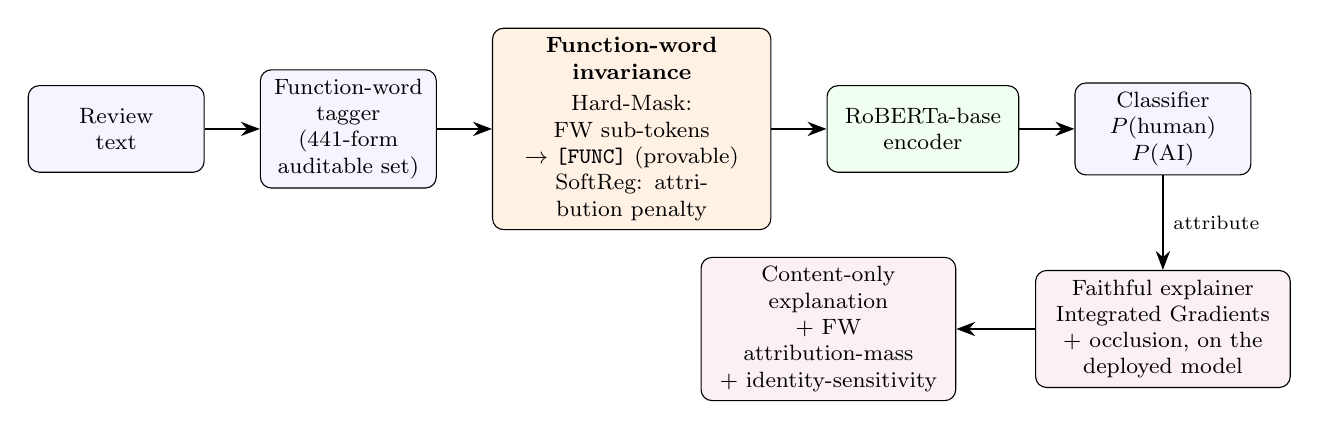
\begin{tikzpicture}[
  font=\footnotesize,
  node distance=6mm and 7mm,
  box/.style={draw,rounded corners,align=center,minimum height=11mm,text width=20mm,fill=blue!4},
  inv/.style={draw,rounded corners,align=center,minimum height=11mm,text width=33mm,fill=orange!10},
  enc/.style={draw,rounded corners,align=center,minimum height=11mm,text width=22mm,fill=green!6},
  expl/.style={draw,rounded corners,align=center,minimum height=11mm,text width=30mm,fill=purple!6},
  arr/.style={-{Stealth[length=2.4mm]},thick},
]
\node[box] (txt) {Review\\text};
\node[box,right=of txt] (tag) {Function-word\\tagger\\(441-form\\auditable set)};
\node[inv,right=of tag] (inv) {\textbf{Function-word invariance}\\[2pt]Hard-Mask: FW sub-tokens\\$\to$ \texttt{[FUNC]} (provable)\\SoftReg: attribution penalty};
\node[enc,right=of inv] (enc) {RoBERTa-base\\encoder};
\node[box,right=of enc] (clf) {Classifier\\$P(\text{human})$\\$P(\text{AI})$};
\node[expl,below=12mm of clf] (expl) {Faithful explainer\\Integrated Gradients\\+ occlusion, on the\\deployed model};
\node[expl,left=10mm of expl] (out) {Content-only explanation\\+ FW attribution-mass\\+ identity-sensitivity};
\draw[arr] (txt) -- (tag);
\draw[arr] (tag) -- (inv);
\draw[arr] (inv) -- (enc);
\draw[arr] (enc) -- (clf);
\draw[arr] (clf) -- (expl) node[midway,right,font=\scriptsize]{attribute};
\draw[arr] (expl) -- (out);
\end{tikzpicture}
\caption{FAITH-Detect architecture. A review is tokenised and its function words are identified by
an auditable surface-form list. The invariance layer then either hard-masks every function-word
sub-token to a shared \texttt{[FUNC]} placeholder (a provable guarantee) or penalises attribution
mass on function words during training (SoftReg); the unconstrained baseline applies neither. A
RoBERTa-base encoder and linear classifier produce the human/AI decision, and a faithful explainer
runs on the \emph{deployed} model to yield content-only explanations and the two reliance metrics.}
\label{fig:arch}
\end{figure*}
\subsection{Function-word set}
The starting point is a precise, reproducible definition of what counts as a function word. Function words are closed-class words---articles, prepositions, conjunctions, auxiliaries, pronouns, particles and determiners---that recur in essentially all English text regardless of author. We compile an auditable English function-word set of 441 surface forms as the union of a curated closed-class list and the standard stop-word lists shipped with NLTK, scikit-learn and spaCy \cite{spacy}. The set is fixed in advance and defined at the surface-form level, which makes identification deterministic at inference time: a word is treated as a function word if its lower-cased, punctuation-stripped form belongs to the set. Because nothing is learned or thresholded here, the same word is classified identically in every document, and the membership test can be audited by simple inspection of the list.
\subsection{Hard-masking (provable function-word-identity invariance)}
The hard-masking variant removes function-word \emph{identity} before the model ever sees it, giving a guarantee rather than a tendency. We tokenise each review with the encoder's byte-level byte-pair-encoding (BPE) tokeniser and map every sub-token back to its surface word using the tokeniser's character offsets. Every sub-token that belongs to a function word is then replaced---\emph{in place}---by a single shared placeholder token, \texttt{[FUNC]}, which we add to the vocabulary. The intuition is simple: if all 441 function words collapse to one indistinguishable symbol, the encoder---and therefore the classifier built on top of it---has no information about which function word originally occurred. The decision is thus invariant to function-word identity by construction, not merely on average.

It is important to be precise about the \emph{scope} of this guarantee, because the replacement is in place: \texttt{[FUNC]} preserves each function word's \emph{position} and the \emph{count} of function-word sub-tokens; only the identity is erased. Consequently the model remains able to read how many closed-class tokens occur and where (we measure this slot reliance in Table~\ref{tab:slotmass}). The guarantee covers exactly those perturbations that leave the masked token sequence unchanged---permuting function words, or swapping a function word for another with the same sub-token segmentation---and it does \emph{not} cover deletion, duplication, or swaps that change a word's sub-token count, all of which alter the \texttt{[FUNC]} positions or counts. This is a constructive and testable property at its stated scope: an automated unit test permutes the function words in a held-out batch and asserts that the model returns bit-identical logits, so the guarantee can be checked rather than assumed. We therefore refer to the property throughout as function-word-\emph{identity} invariance, never as invariance to function words in general.
\subsection{Soft attribution regularisation}
The soft variant pursues the same goal of low function-word reliance, but as a learned preference instead of an architectural guarantee. It keeps the full, unmodified text and adds a training penalty that discourages the model from placing explanatory weight on function words \cite{ross}. Concretely, let $x$ be the input tokens with label $y$, let $g_i = \partial f_\theta(x)_y / \partial e_i \cdot e_i$ be the gradient-times-input saliency of token $i$ (with $e_i$ its embedding), and let $\mathcal{F}$ index the function-word tokens. We train with
\begin{equation}
\mathcal{L} \;=\; \mathcal{L}_{\mathrm{CE}}(f_\theta(x), y) \;+\; \lambda \,\frac{\sum_{i \in \mathcal{F}} |g_i|}{\sum_{j} |g_j|},
\label{eq:softreg}
\end{equation}
where $\mathcal{L}_{\mathrm{CE}}$ is the cross-entropy loss and the second term is the fraction of input-gradient saliency that lands on function-word tokens. The saliency is computed with \texttt{create\_graph} enabled, so this penalty is itself differentiable and back-propagates into the network weights, steering the model towards explanations supported by content. Because the penalty is second order, evaluating it over a full large batch is memory-intensive; we therefore estimate it on a small random sub-batch---an unbiased stochastic estimate of the same quantity---while the cross-entropy term still uses the full batch.
\subsection{Faithful, content-only explanations}
The final stage explains decisions in a way that is faithful to the model that actually made them. By faithful we mean that the attributions reflect the deployed network's own computation rather than an approximation: all attributions are computed on the deployed model---including the hard-masking transform when it is active---and never on a separate surrogate classifier. We use two complementary attribution methods, aggregated to the word level: Integrated Gradients on the embedding layer \cite{ig}, a gradient-based measure, and leave-one-word-out occlusion, a perturbation-based measure. Function words are then excluded from the explanation that is shown to a user, so the displayed evidence is \emph{content-displayed} by construction. We are careful with this term: it is a property of what the explanation shows (content words, on the deployed model), not a claim that the shown content fully captures the decision---which, given the slot reliance measured in Table~\ref{tab:slotmass}, it does not.

To make function-word reliance directly measurable rather than merely asserted, we report two reliance metrics. The first is the \emph{function-word attribution mass}, the share of the model's total absolute attribution that falls on function words,
\begin{equation}
\mathrm{FWM} \;=\; \frac{\sum_{i \in \mathcal{F}} |a_i|}{\sum_{j} |a_j|},
\label{eq:fwm}
\end{equation}
where $a_i$ is the attribution of token $i$; a value of zero means the model places no explanatory weight on function words. The second is the \emph{identity-sensitivity} metric, a forward-only probe defined as the mean absolute change in the predicted AI probability when each function word is swapped for a different function word,
\begin{equation}
\mathrm{IDS} \;=\; \mathbb{E}\!\left[\,\big|\,p(\text{AI}\mid x) - p(\text{AI}\mid x')\,\big|\,\right],
\label{eq:ids}
\end{equation}
where $x'$ is $x$ with one function word replaced by another. The two metrics view the same underlying property---reliance on function-word identity---from the gradient side (Eq.~\ref{eq:fwm}) and the perturbation side (Eq.~\ref{eq:ids}), and the hard-masking guarantee forces both towards zero. For explanation quality we additionally report ERASER comprehensiveness and sufficiency \cite{eraser} and deletion/insertion AUC computed over content words \cite{rise}.

\section{Experimental Setup}
This section describes the data, the splits, and the protocol used to train and evaluate every model in the paper. We keep three goals in view throughout: leakage-free measurement, multi-seed reporting with confidence intervals, and a like-for-like comparison between the unconstrained baseline and the two function-word-identity-invariant variants.

\subsection{Datasets}
We use three corpora, each playing a distinct role. First, an in-domain benchmark on which all models are trained. Second, an out-of-distribution (OOD) set that shifts both the writing domain and the generating model. Third, a second corpus used only to check that our findings replicate.

\textbf{In-domain: MAiDE-up (English hotel reviews).} Our primary benchmark is the English subset of MAiDE-up \cite{maideup}, a collection of roughly 2{,}000 hotel reviews labelled as either human-written or generated by GPT-4. Because the two classes share the same hotels, the dataset is well matched in topic, which forces a detector to learn the human--machine distinction rather than the topic. This matching also creates a subtle hazard. Every hotel appears in \emph{both} classes, so a random train--test split places reviews of the same hotel on both sides of the boundary. A model can then memorise hotel-specific content (named amenities, locations, recurring phrases) and inflate its score without learning anything about authorship---a form of leakage. To prevent this, we partition by hotel rather than by review: all reviews of a given hotel fall entirely within one split. Concretely, the grouped splits contain 1{,}400 training, 200 validation and 400 test reviews, with zero train--test hotel overlap (Figure~\ref{fig:01_dataset_overview}). We additionally report a random split later in the paper to quantify exactly how much the leakage inflates scores, but every headline number uses the grouped, leakage-free split.

\textbf{Out-of-distribution: RAID reviews.} To probe transfer, we evaluate on the reviews domain of the RAID benchmark \cite{raid}. This set differs from MAiDE-up along two axes at once. The domain shifts (hotel reviews to other review text), and the machine text comes from \emph{multiple} generators rather than a single one---including GPT-3.5 and GPT-4, Cohere and Llama. RAID therefore stresses both content-vocabulary shift and generator diversity, and serves as a deliberately hard test of whether an in-domain detector still works when the surrounding distribution changes.

\textbf{Replication: HC3.} Finally, we use the HC3 corpus (human answers versus ChatGPT answers) as an independent corpus on which to repeat the core comparison. It lets us check whether the trade-offs we observe on MAiDE-up are properties of a single dataset or recur on unrelated text; the full HC3 analysis appears in the Results.

\subsection{Training and evaluation protocol}
\textbf{Model and optimisation.} Unless stated otherwise, every neural detector is a fine-tuned \texttt{roberta-base} encoder \cite{roberta} with a linear classification head, trained with the AdamW optimiser \cite{adamw}. To make the comparison statistically meaningful rather than anecdotal, we train each configuration under five random seeds and report the mean together with a 95\% confidence interval (CI). Reporting an interval, rather than a single best run, lets the reader see when two models are genuinely separated and when an apparent gap is within sampling noise.

\textbf{Two experimental scales.} We distinguish, explicitly and throughout, two scales of experiment. \emph{Main} results---in-domain performance, the primary attacks, cross-domain transfer, reliance, faithfulness, calibration and leakage---use the full configuration above: \texttt{roberta-base}, five seeds, and the full MAiDE-up training set (1,400 reviews). A number of \emph{targeted analyses}---mixed-generator training, the per-category and attack-type decompositions, slot-attribution mass, few-shot recovery, and the HC3 replication---are run at \emph{pilot} scale: \texttt{distilroberta-base} on a 600-review subsample (and only two seeds for HC3). Pilot results are labelled as such in every caption; we treat their effect sizes as indicative and their absolute values as not directly comparable to the main \texttt{roberta-base} numbers, and we release the protocols so each can be reproduced at full scale.

\textbf{Robustness attacks.} We probe robustness with two complementary text attacks applied at evaluation time. The function-word attack deletes, duplicates and swaps function words, directly perturbing the cue this paper studies; a detector that ignores function-word identity should be unmoved by it. The synonym attack replaces content words with WordNet \cite{wordnet} synonyms, perturbing the very signal the masked model must rely on; it therefore tests the opposite extreme. Together the two attacks bracket the detector's exposure: one targets the cue we remove, the other targets the cue we keep.

\textbf{Baselines.} Alongside the neural models we include two classic detectors so the transformer results have a simple, transparent reference. Both are TF-IDF features fed to a logistic-regression classifier: a full-vocabulary variant and a content-only variant that drops function words. These baselines require no GPU, are easy to reproduce, and indicate how much of the task is solvable with surface word statistics alone.

\textbf{Significance testing.} We avoid resting any claim on a single point estimate. For two models compared on the same shared test set we use McNemar's test, which is appropriate for paired predictions on identical examples. Confidence intervals over seeds use the Student-$t$ distribution, and we cross-check them with the bootstrap. Where we report that two models are statistically indistinguishable, or that one transfers worse with non-overlapping intervals, these are the tests behind the statement.

\begin{figure}[tb]\centering
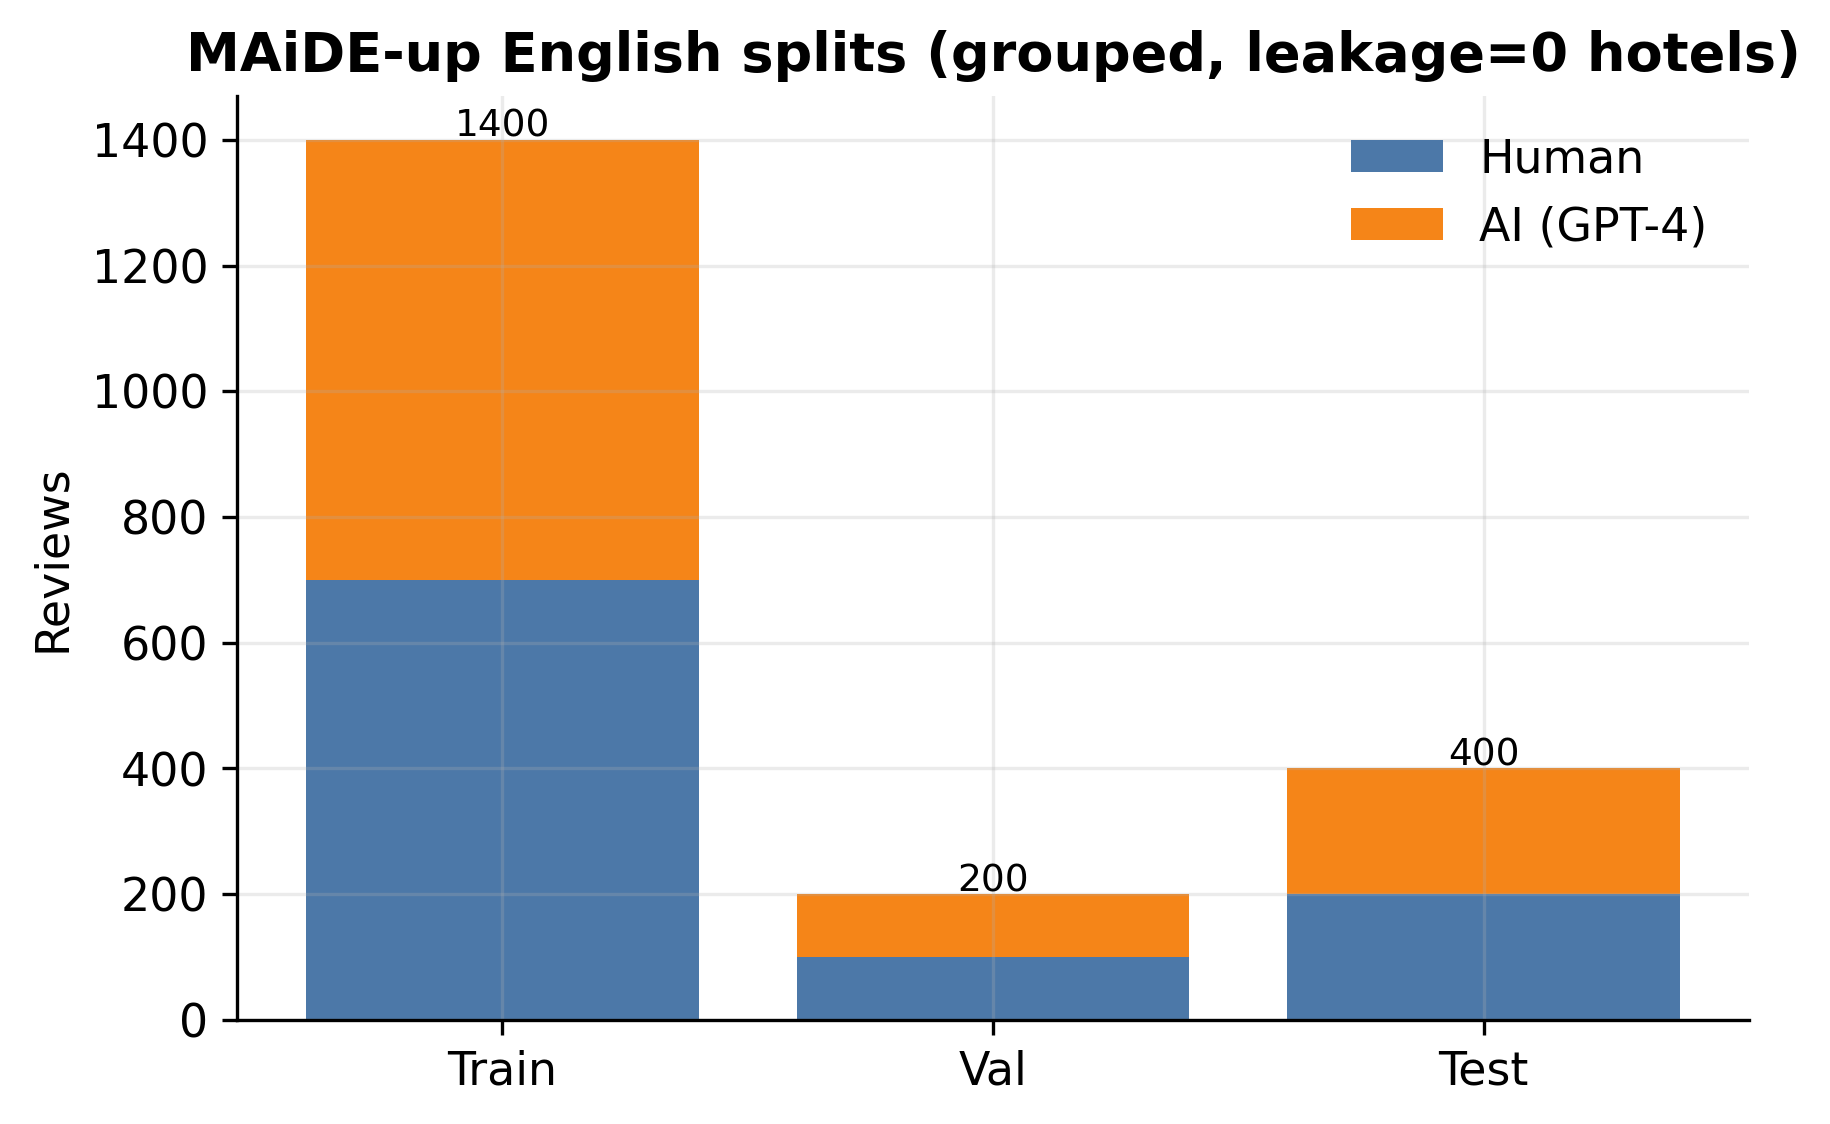
\includegraphics[width=\linewidth]{figures/01_dataset_overview.png}
\caption{MAiDE-up English splits, grouped by hotel so that no hotel appears in both training and test (zero train--test leakage).}
\label{fig:01_dataset_overview}
\end{figure}

\section{Results}

\subsection{In-domain performance}
We begin with the easiest test: detection on the same distribution the model was trained on. Here a detector sees hotel reviews from the same source, by the same generator (GPT-4), as in training, so this measures the ceiling of what each variant can achieve before any shift is introduced. Table~\ref{tab:indomain} reports macro F1, ROC-AUC and accuracy as mean $\pm$ 95\% confidence interval over five seeds.

\begin{table}[tb]\centering
\caption{In-domain performance (mean $\pm$ 95\% CI over seeds; \% units).}
\label{tab:indomain}
\footnotesize
\begin{tabular}{lccc}
\toprule
Model & F1 (macro) & ROC-AUC & Accuracy \\
\midrule
Baseline & 93.7 $\pm$ 2.8 & 99.4 $\pm$ 0.3 & 93.8 $\pm$ 2.8 \\
SoftReg & 93.8 $\pm$ 3.6 & 99.3 $\pm$ 0.4 & 93.8 $\pm$ 3.5 \\
Hard-Mask (FAITH) & 93.6 $\pm$ 1.7 & 98.6 $\pm$ 0.6 & 93.6 $\pm$ 1.7 \\
tfidf\_lr & 92.2 & 97.9 & 92.2 \\
tfidf\_lr\_content & 91.7 & 97.2 & 91.8 \\
\bottomrule
\end{tabular}
\end{table}

The central in-domain finding is that the three neural variants are statistically indistinguishable. A McNemar test comparing the unconstrained baseline against Hard-Mask gives $p=0.15$, so we cannot reject the hypothesis that the two models make the same errors on the shared test set. Concretely, this means the differences in Table~\ref{tab:indomain} are within the noise of seed variation: forcing the detector to ignore function-word identity does not cost it any measurable in-domain accuracy on this benchmark. Hard-Mask reaches the same macro F1 as the baseline (93.6 vs.\ 93.7) and in fact does so with the tightest confidence interval ($\pm$1.7), indicating it is also the most stable across seeds. The classic TF-IDF baselines trail the neural models by roughly one to two points, which confirms that the task is largely linearly separable in-domain but that the transformer still extracts a little extra signal.

In short, function-word-identity invariance is free here: the provable guarantee built into Hard-Mask buys robustness and faithful explanations (shown below) without sacrificing in-domain performance (Figure~\ref{fig:03_indomain_performance}). The confusion matrices (Figure~\ref{fig:04_confusion_matrices}) and the ROC and precision--recall curves (Figure~\ref{fig:05_roc_pr}) reproduce the same ordering, with very high ROC-AUC for all three neural variants and no systematic asymmetry between the human and AI classes.

\begin{figure}[tb]\centering

\includegraphics[width=\linewidth]{figures/03_indomain_performance.png}
\caption{In-domain F1 (mean $\pm$ 95\% CI) with classic baselines.}
\label{fig:03_indomain_performance}
\end{figure}
\begin{figure*}[tp]\centering

\includegraphics[width=\textwidth]{figures/04_confusion_matrices.png}
\caption{In-domain confusion matrices (reference seed) by variant.}
\label{fig:04_confusion_matrices}
\end{figure*}
\begin{figure*}[tp]\centering

\includegraphics[width=\textwidth]{figures/05_roc_pr.png}
\caption{In-domain ROC and precision--recall curves (reference seed).}
\label{fig:05_roc_pr}
\end{figure*}

\subsection{Training-free (zero-shot) baselines}\label{sec:zeroshot}
We next ask how far one can get without any labelled training data at all. Training-free (also called zero-shot) detectors flag machine text purely from the statistics of a scoring language model, with no supervised fine-tuning. They are a useful reference point because they require no labels and expose what is detectable from likelihood alone. Table~\ref{tab:zeroshot} reports four such methods.

\begin{table*}[tp]\centering
\caption{Training-free detectors (GPT-2-scored; thresholds fit on the training split only; \% units for F1).}
\label{tab:zeroshot}
\footnotesize
\begin{tabular}{lccc}
\toprule
Method & In-domain F1 / AUROC & FW-attack F1 & OOD F1 / AUROC \\
\midrule
loglik & 74.2 / 0.81 & 35.5 & 45.6 / 0.78 \\
logrank & 71.7 / 0.79 & 33.9 & 48.3 / 0.79 \\
entropy & 70.0 / 0.75 & 40.9 & 46.8 / 0.71 \\
fast-detectgpt & 71.2 / 0.80 & 33.2 & 54.0 / 0.75 \\
\bottomrule
\end{tabular}
\end{table*}

The four detectors are: mean log-likelihood, log-rank \cite{gltr}, predictive entropy, and the analytic Fast-DetectGPT discrepancy \cite{fastdetectgpt}. Each scores a review with GPT-2 and is thresholded on the training split only, so no test-time labels leak in.\footnote{Our entropy score is oriented so that \emph{lower} entropy indicates machine text, which is the empirically correct direction on this dataset and the opposite of the convention in some prior work; AUROC is unaffected by orientation up to reflection.}

Two patterns stand out. First, all four trail the supervised models in-domain by a wide margin: their F1 sits in the low-to-mid 70s against roughly 94 for the fine-tuned transformers. This gap is expected on a single-domain benchmark, where a supervised model can learn the exact content vocabulary that separates the two classes, whereas a likelihood detector only sees how ``surprising'' the text is to GPT-2. We therefore report these numbers to contextualise the supervised results, not as competitors; their value is that they need no labelled data and still recover most of the signal.

Second, the zero-shot detectors are not immune to function-word perturbation. Under the function-word attack their F1 shifts by an average of $+35.9$ points, confirming that likelihood-based statistics also respond strongly to function-word edits---deleting, duplicating or swapping closed-class tokens changes the sentence-level probabilities these methods rely on. This matters for the wider argument of the paper: function-word sensitivity is not peculiar to supervised transformers but appears across detector families. Only the hard-masked model is invariant to such edits by construction, because it never sees function-word identity in the first place.

\subsection{Function-word reliance}
Having established in-domain parity, we now quantify the property that motivates the method: how much each detector actually relies on function words. It is important to separate two senses of ``reliance'' that the rest of this paper keeps distinct. The first is reliance on function-word \emph{identity}---which particular closed-class word appears (``the'' vs.\ ``a''). The second is reliance on function-word \emph{slots}---the positions and counts of closed-class tokens, independent of which word fills them. Hard masking removes the first by construction but, as we show below, leaves the second intact: it replaces every function word with the same \texttt{[FUNC]} placeholder, so the slot (and its position) survives even though its identity is erased.

We first measure reliance on identity, two complementary ways. The first is function-word attribution mass: the share of the model's total absolute Integrated-Gradients attribution that lands on function-word tokens. The second is identity-sensitivity: the mean change in the predicted AI probability when each function word is replaced by a different function word. The first is gradient-based and the second is a forward-only perturbation, so agreement between them is strong evidence rather than an artefact of one technique. Table~\ref{tab:reliance} reports both.

\begin{table}[tb]\centering
\caption{Reliance on function-word \emph{identity} (full run: roberta-base, 5 seeds): attribution mass on function-word tokens and identity-sensitivity. Lower is less reliance. This measures identity only; slot reliance is in Table~\ref{tab:slotmass}.}
\label{tab:reliance}
\footnotesize
\begin{tabular}{lcc}
\toprule
Variant & \shortstack{FW attribution\\mass (IG)} & \shortstack{Identity-\\sensitivity $|\Delta p|$} \\
\midrule
Baseline & 36.5\% & 10.93\% \\
SoftReg & 30.0\% & 10.61\% \\
Hard-Mask (FAITH) & 0.0\% & 0.72\% \\
\bottomrule
\end{tabular}
\end{table}

The identity numbers describe a clear progression. The unconstrained baseline places a substantial 36.5\% of its attribution on function words---more than a third of its evidence comes from tokens that intuitively should carry little signal about authenticity. Soft regularisation pulls this down to 30.0\%, confirming that the attribution penalty pushes evidence toward content as intended, though it does not remove function-word reliance entirely. Hard masking drives it to exactly 0.0\% (Figure~\ref{fig:08_fw_attribution_mass}). We stress what this zero does and does not mean. It is a structural consequence of the construction: because every function word is replaced by the same \texttt{[FUNC]} placeholder, the model cannot distinguish which function word occurred, so its attribution to function-word \emph{identity} is necessarily zero. It is \emph{not} a statement that Hard-Mask ignores the function-word slots---that question is answered separately, and differently, below.

The identity-sensitivity metric agrees from the perturbation side (Figure~\ref{fig:08b_fw_identity_sensitivity}). Swapping function words for other function words moves the baseline's AI probability by 10.93\% on average but barely changes Hard-Mask (0.72\%, near-zero and attributable to numerical noise). Together the two metrics certify exactly what the construction promises and no more: for Hard-Mask the decision cannot depend on \emph{which} function word appeared.

\paragraph{Reliance on the slots, not the identity.} A natural objection---and one we think is the most important caveat in this paper---is that a model can still lean heavily on the function-word \emph{slots} (their positions and counts) even when their identity is hidden. The attribution-mass metric above cannot see this, because the standard Integrated-Gradients baseline treats the added \texttt{[FUNC]} token as a special token and so assigns it exactly zero attribution by construction (the very artefact that produces the headline 0.0\%). We therefore measure slot reliance directly, two ways: Integrated Gradients with a \emph{pad} baseline at the \texttt{[FUNC]} positions (so the placeholder's contribution is actually measured, comparably to how function-word mass is measured for the other variants), and forward-only occlusion (deleting each \texttt{[FUNC]} slot and recording the change in AI probability). Table~\ref{tab:slotmass} reports both at pilot scale (distilroberta-base, seed 0). The result is unambiguous: Hard-Mask places \textbf{18.2\%} of its gradient attribution and \textbf{34.9\%} of its occlusion-measured reliance on the \texttt{[FUNC]} slots---comparable to the baseline's reliance on function words (37.6\% by occlusion; Figure~\ref{fig:slotmass}). In other words, Hard-Mask is invariant to function-word \emph{identity} (proven) but is \emph{not} invariant to function-word \emph{slots}: it still reads how many closed-class tokens occur and where. This sharpens, rather than weakens, the paper's claim---the guarantee is precisely about identity---and it is the reason we are careful, in \S\ref{sec:faith}, not to overclaim faithfulness.

\begin{table}[tb]\centering
\caption{Attribution on function-word \emph{slots} (the \texttt{[FUNC]} positions for Hard-Mask), pilot scale (distilroberta-base, seed 0). Hard-Mask removes function-word identity (Table~\ref{tab:reliance}) yet still places substantial attribution on the slots.}
\label{tab:slotmass}
\footnotesize
\begin{tabular}{lcc}
\toprule
Variant & \shortstack{IG slot mass\\(pad baseline)} & \shortstack{Occlusion\\slot mass} \\
\midrule
Baseline & 35.4\% & 37.6\% \\
SoftReg & 24.3\% & 39.1\% \\
Hard-Mask (FAITH) & 18.2\% & 34.9\% \\
\bottomrule
\end{tabular}
\end{table}

\begin{figure}[tb]\centering
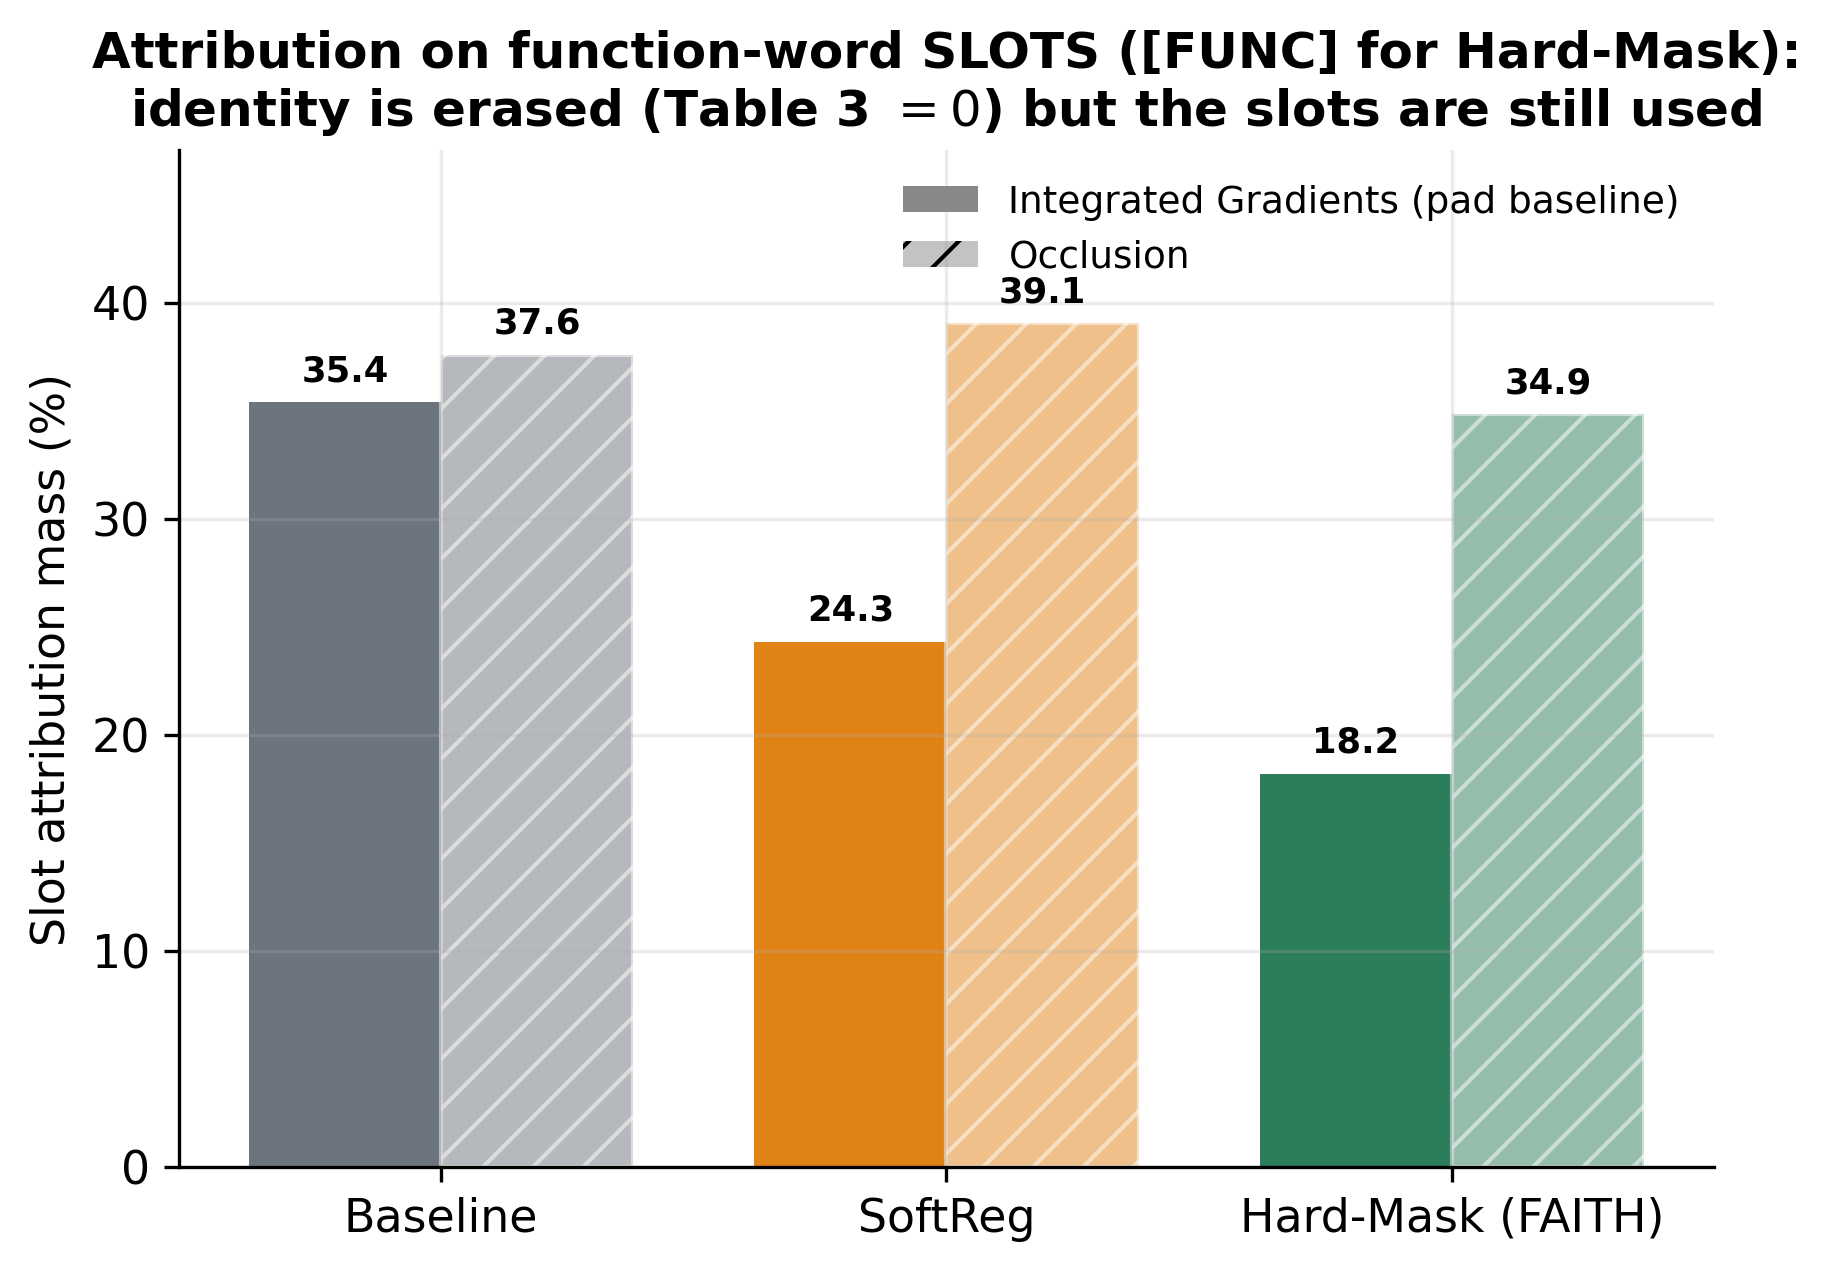
\includegraphics[width=\linewidth]{figures/slot_attribution_mass.png}
\caption{Attribution on function-word \emph{slots} (the \texttt{[FUNC]} positions for Hard-Mask). Hard-Mask erases function-word identity (Table~\ref{tab:reliance} reports $0\%$) yet still routes $18.2\%$ (IG) and $34.9\%$ (occlusion) of its attribution through the slots---comparable to the baseline.}
\label{fig:slotmass}
\end{figure}

\begin{figure}[tb]\centering
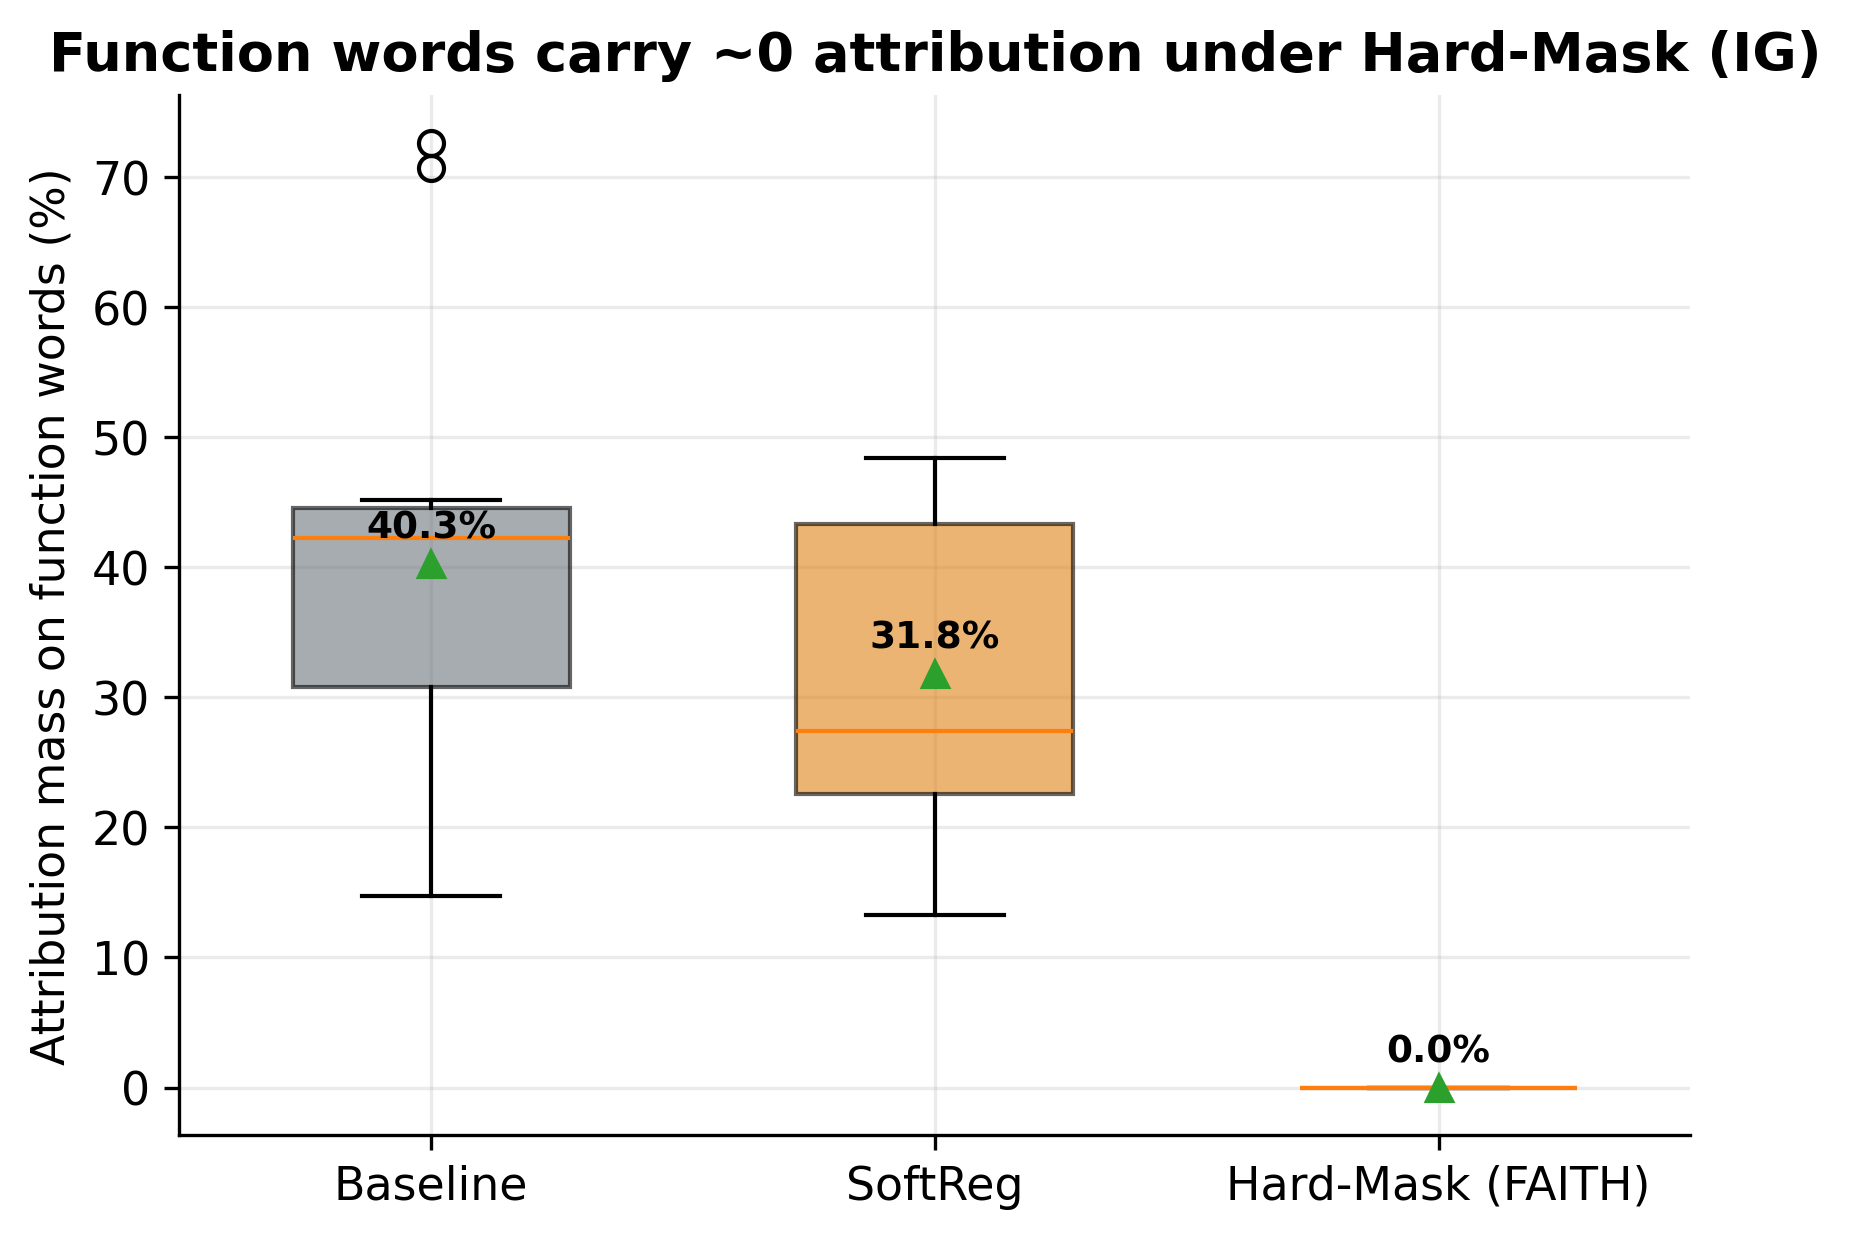
\includegraphics[width=\linewidth]{figures/08_fw_attribution_mass.png}
\caption{Integrated-Gradients attribution mass on function-word \emph{identity} (full run). This is the identity mass that hard masking drives to zero; the residual reliance on the \texttt{[FUNC]} \emph{slots} is shown separately in Figure~\ref{fig:slotmass}.}
\label{fig:08_fw_attribution_mass}
\end{figure}
\begin{figure}[tb]\centering

\includegraphics[width=\linewidth]{figures/08b_fw_identity_sensitivity.png}
\caption{Change in AI probability when function words are swapped.}
\label{fig:08b_fw_identity_sensitivity}
\end{figure}

\subsection{Robustness to text attacks}
The reliance metrics predict how each variant should behave under attack, and the robustness experiments test that prediction directly. We probe two attacks. The function-word attack perturbs closed-class words (deleting, duplicating or swapping them), leaving content untouched. The synonym attack replaces content words with WordNet \cite{wordnet} synonyms, leaving function words untouched. Table~\ref{tab:robust} reports macro F1 on clean text and under each attack, averaged over seeds. We then decompose the function-word attack, because---following the slot/identity distinction of the previous subsection---the invariance guarantee covers only one of its three operations. A \emph{swap} changes a function word's identity; if the replacement has the same sub-token segmentation, the hard-masked input is unchanged and the proof applies. \emph{Deletion} and \emph{duplication}, by contrast, change the number and position of \texttt{[FUNC]} slots, which the model can see, so they are \emph{not} covered by the guarantee. Table~\ref{tab:attacksplit} reports the decomposition.

\begin{table}[tb]\centering
\caption{F1 (macro) under text attacks (mean over seeds; \% units).}
\label{tab:robust}
\footnotesize
\begin{tabular}{lccc}
\toprule
Variant & Clean & function word & synonym \\
\midrule
Baseline & 93.7 & 87.2 & 88.4 \\
SoftReg & 93.8 & 87.0 & 86.4 \\
Hard-Mask (FAITH) & 93.6 & 95.8 & 89.9 \\
\bottomrule
\end{tabular}
\end{table}

Under the function-word attack the result follows directly from invariance. The baseline and soft variants each lose several points (down to 87.2 and 87.0), because they rely on function words that the attack manipulates. Hard-Mask, in contrast, is essentially unaffected: its F1 of 95.8 is statistically flat against its clean score (Figure~\ref{fig:07_robustness}). The reason is mechanical, not coincidental---a perturbation that only touches function words cannot move a decision that, by construction, never reads function-word identity. This is exactly the behaviour the reliance metrics predicted, and it is why we describe Hard-Mask as flat under the function-word attack rather than merely robust to it.

Under synonym substitution the picture is less absolute, because this attack edits the content words that all three models do read. Every variant therefore degrades. The informative point is the ordering: Hard-Mask degrades least and retains the highest F1 (89.9), suggesting that by forcing the model onto content it learns a more distributed, less brittle content representation rather than leaning on a few fragile lexical cues. We regard these two attacks as the clearest empirical benefits of invariance, and we limit the claim accordingly: we demonstrate robustness to the two attacks tested and do not extrapolate to adversarial pressure in general.

\paragraph{Decomposing the function-word attack.} Table~\ref{tab:attacksplit} and Figure~\ref{fig:attacksplit} separate swap, deletion and duplication (pilot scale, distilroberta-base, seed 0; absolute values differ from Table~\ref{tab:robust}, which is the full-scale combined attack, so the informative quantity is the per-operation pattern). Two things stand out. First, under the \emph{swap} (identity-only) attack Hard-Mask is essentially unmoved ($91.5\to92.2$), whereas the baseline drops ($92.7\to88.4$) and SoftReg collapses ($95.5\to77.2$). This is the operation the proof covers, and it is exactly where invariance pays off---and, strikingly, where the soft variant is \emph{most} fragile, because it learns to lean on function-word identity that the attack then rewrites. Second, under deletion and duplication---which the guarantee does \emph{not} cover, since they move and recount the \texttt{[FUNC]} slots Hard-Mask can see---all three variants move modestly and Hard-Mask enjoys no special protection ($91.5\to90.2$ under deletion). The decomposition therefore states the guarantee precisely: Hard-Mask is invariant to function-word \emph{identity} (swap), not to perturbations of the \emph{slots} (deletion/duplication), consistent with the slot-reliance finding above. The small residual swap movement ($+0.7$) reflects swaps that change a word's sub-token count and thus the number of \texttt{[FUNC]} tokens, which the exact-permutation guarantee (asserted bit-identically by our invariance test) does not include.

\begin{table}[tb]\centering
\caption{Function-word attack decomposed (macro F1 \%; pilot: distilroberta-base, seed 0). Swap = identity-only (proof covers it); delete/duplicate change \texttt{[FUNC]} positions/counts (not covered).}
\label{tab:attacksplit}
\footnotesize
\begin{tabular}{lcccc}
\toprule
Variant & Clean & Swap & Delete & Duplicate \\
\midrule
Baseline & 92.7 & 88.4 & 95.0 & 94.7 \\
SoftReg & 95.5 & 77.2 & 88.1 & 94.7 \\
Hard-Mask (FAITH) & 91.5 & 92.2 & 90.2 & 92.2 \\
\bottomrule
\end{tabular}
\end{table}

\begin{figure}[tb]\centering
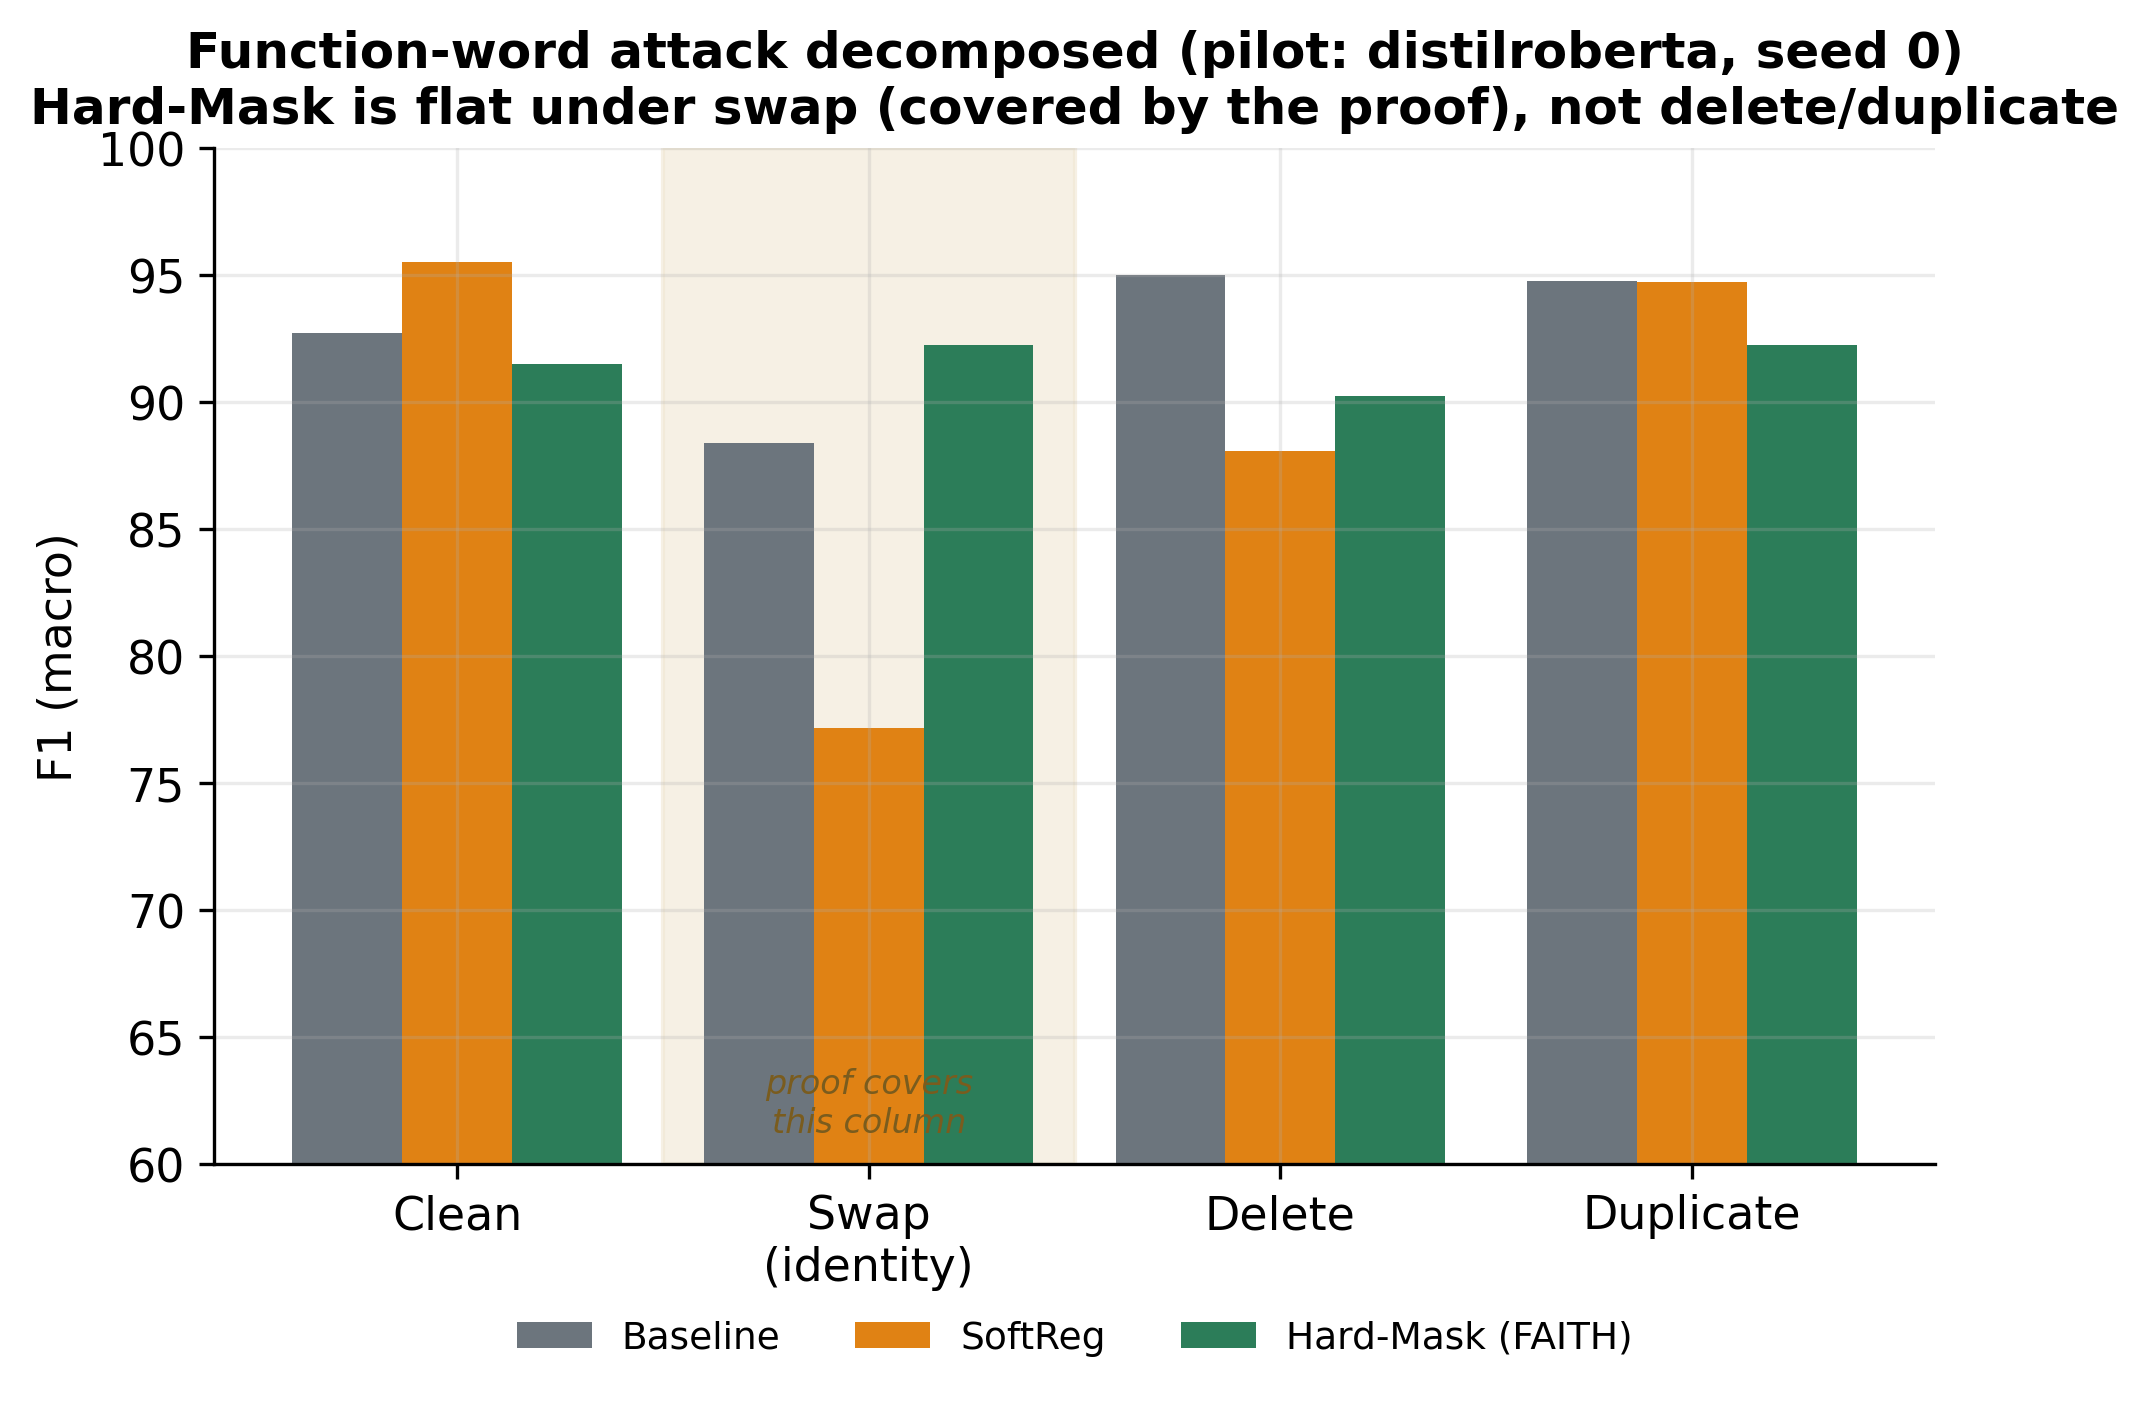
\includegraphics[width=\linewidth]{figures/attack_split.png}
\caption{The function-word attack decomposed (pilot). Under the \emph{swap} (identity) attack---the only operation the proof covers---Hard-Mask is flat while SoftReg collapses; deletion and duplication, which move the \texttt{[FUNC]} slots, are not covered and move all variants.}
\label{fig:attacksplit}
\end{figure}

\begin{figure}[tb]\centering

\includegraphics[width=\linewidth]{figures/07_robustness.png}
\caption{F1 under text attacks; Hard-Mask is flat under the function-word attack.}
\label{fig:07_robustness}
\end{figure}

\subsection{Cross-domain and cross-generator transfer}
So far function-word-identity invariance has looked free or beneficial. This subsection is where the trade-off appears. We move the in-domain detectors, unchanged, to a different distribution and ask how well they transfer.
\begin{table*}[tp]\centering
\caption{In-domain vs.\ cross-domain OOD (mean $\pm$ 95\% CI). F1 in \% units; ROC-AUC and PR-AUC in $[0,1]$. The threshold-free ranking metrics (ROC-AUC, PR-AUC) show a far smaller Hard-Mask gap than F1 does, indicating that much of the F1 collapse is a threshold/operating-point effect.}
\label{tab:ood}
\footnotesize
\begin{tabular}{lcccc}
\toprule
Variant & In-domain F1 & OOD F1 & OOD ROC-AUC & OOD PR-AUC \\
\midrule
Baseline & 93.7 $\pm$ 2.8 & 69.5 $\pm$ 7.5 & 0.780 $\pm$ 0.026 & 0.825 $\pm$ 0.018 \\
SoftReg & 93.8 $\pm$ 3.6 & 68.2 $\pm$ 10.1 & 0.779 $\pm$ 0.018 & 0.823 $\pm$ 0.007 \\
Hard-Mask (FAITH) & 93.6 $\pm$ 1.7 & 47.4 $\pm$ 8.3 & 0.764 $\pm$ 0.041 & 0.777 $\pm$ 0.039 \\
\bottomrule
\end{tabular}
\end{table*}
On the cross-domain out-of-distribution (OOD) set---hotel reviews at training time, movie reviews at test time---the picture reverses. Hard-Mask now transfers \emph{worse} than the baseline, and the gap is large enough that the 95\% confidence intervals do not overlap (Figure~\ref{fig:06_ood_transfer}). The intuition is direct. Hard-Mask is forced to decide using content words alone, and the content vocabulary of hotel reviews (rooms, breakfast, check-in) barely overlaps with that of movie reviews (plot, acting, direction). When that vocabulary shifts, the features Hard-Mask relies on largely vanish. The baseline, by contrast, can still lean on function-word and stylistic regularities, and these evidently carry signal that survives the domain change. In short, function words are not pure noise: under cross-domain transfer they can be genuinely useful, which is exactly why removing them hurts here.

\paragraph{How much of the gap is the threshold?} The F1 column overstates the collapse. F1 is computed at a fixed decision threshold, and a threshold tuned in-domain need not suit a shifted distribution; the threshold-free ranking metrics are the fairer test of whether the model can still tell human from machine OOD. By ROC-AUC the Hard-Mask gap nearly disappears---$0.764$ versus the baseline's $0.780$, with overlapping intervals---and by PR-AUC it is $0.777$ versus $0.825$. In other words, Hard-Mask still \emph{ranks} OOD reviews almost as well as the baseline; what degrades sharply is the calibrated operating point, not the underlying separability. This both tempers the headline (the cross-domain ``cost'' is smaller than the $47.4$ vs $69.5$ F1 suggests) and points to a cheap fix: re-tuning the threshold, or the light few-shot adaptation of \S\ref{sec:fewshot}, recovers much of the F1 without retraining. We report F1 for continuity with the rest of the paper but treat the AUROC/PR-AUC columns as the more reliable cross-domain comparison (Figure~\ref{fig:oodthreshold}).

\begin{figure}[tb]\centering
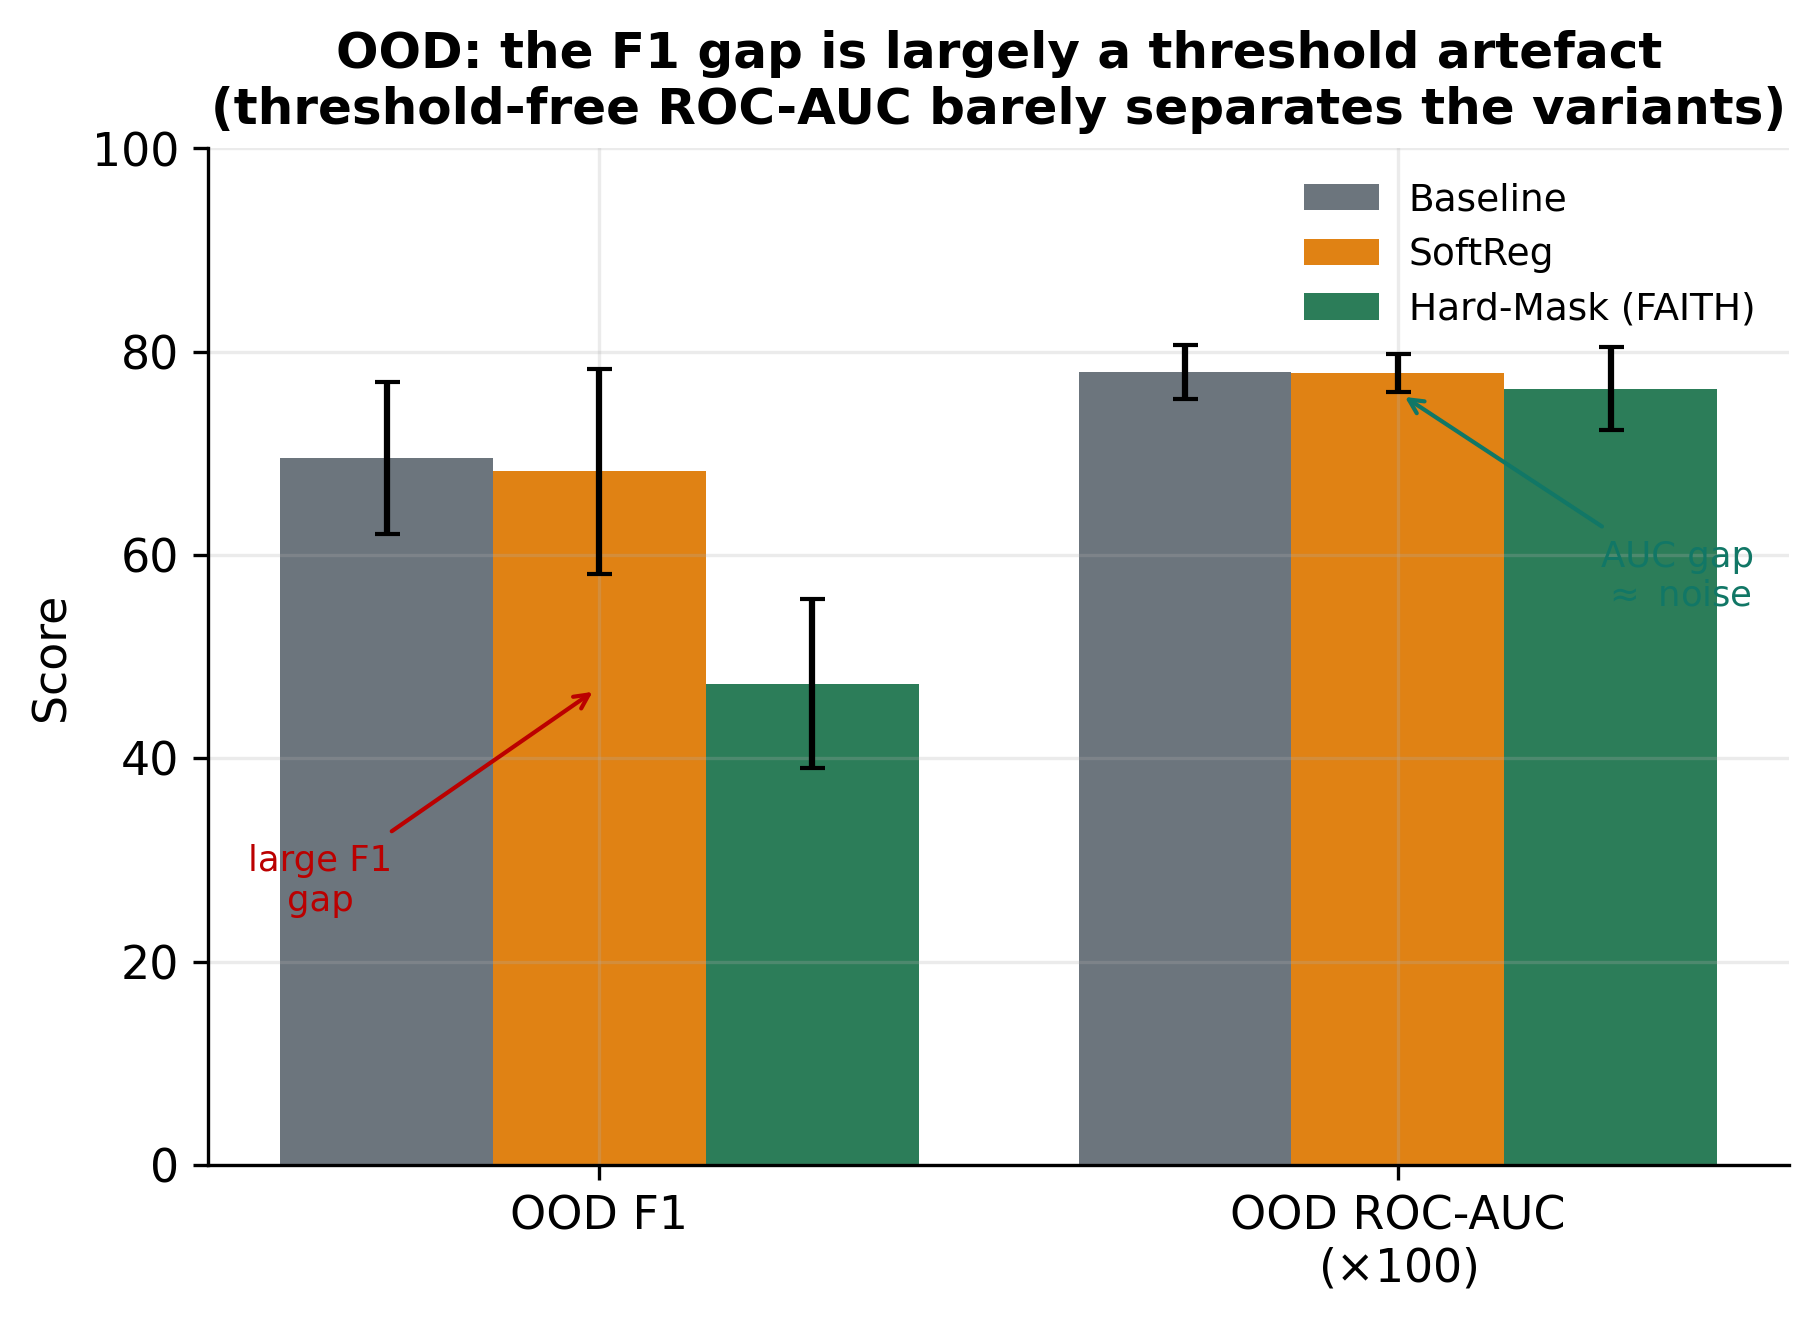
\includegraphics[width=\linewidth]{figures/ood_threshold.png}
\caption{The cross-domain ``cost'' is largely an operating-point effect. Hard-Mask's OOD \emph{F1} drops well below the baseline (left), but the threshold-free \emph{ROC-AUC} gap is within noise (right)---the model still ranks OOD reviews almost as well; only the calibrated threshold degrades.}
\label{fig:oodthreshold}
\end{figure}

The per-generator breakdown tells a consistent story. Figure~\ref{fig:06b_cross_generator} reports detection F1 separately for each generator in the RAID reviews pool, and the same ordering---baseline ahead of Hard-Mask---holds across most of them, so the reversal is not driven by a single anomalous generator.

We stress one important confound before drawing any conclusion about generators. This OOD test changes \emph{both} the domain (hotels to movies) and the generator mix (GPT-4 to a broader set including GPT-3.5/4, Cohere and Llama) at the same time, and the domain change is extreme. It therefore cannot isolate cross-generator transfer on its own: a same-domain, different-generator test is needed to make that claim cleanly, which is precisely the experiment we run in \S\ref{sec:mixedgen}.
\begin{figure}[tb]\centering

\includegraphics[width=\linewidth]{figures/06_ood_transfer.png}
\caption{In-domain vs.\ cross-domain OOD F1 by variant (mean $\pm$ 95\% CI).}
\label{fig:06_ood_transfer}
\end{figure}
\begin{figure*}[tp]\centering
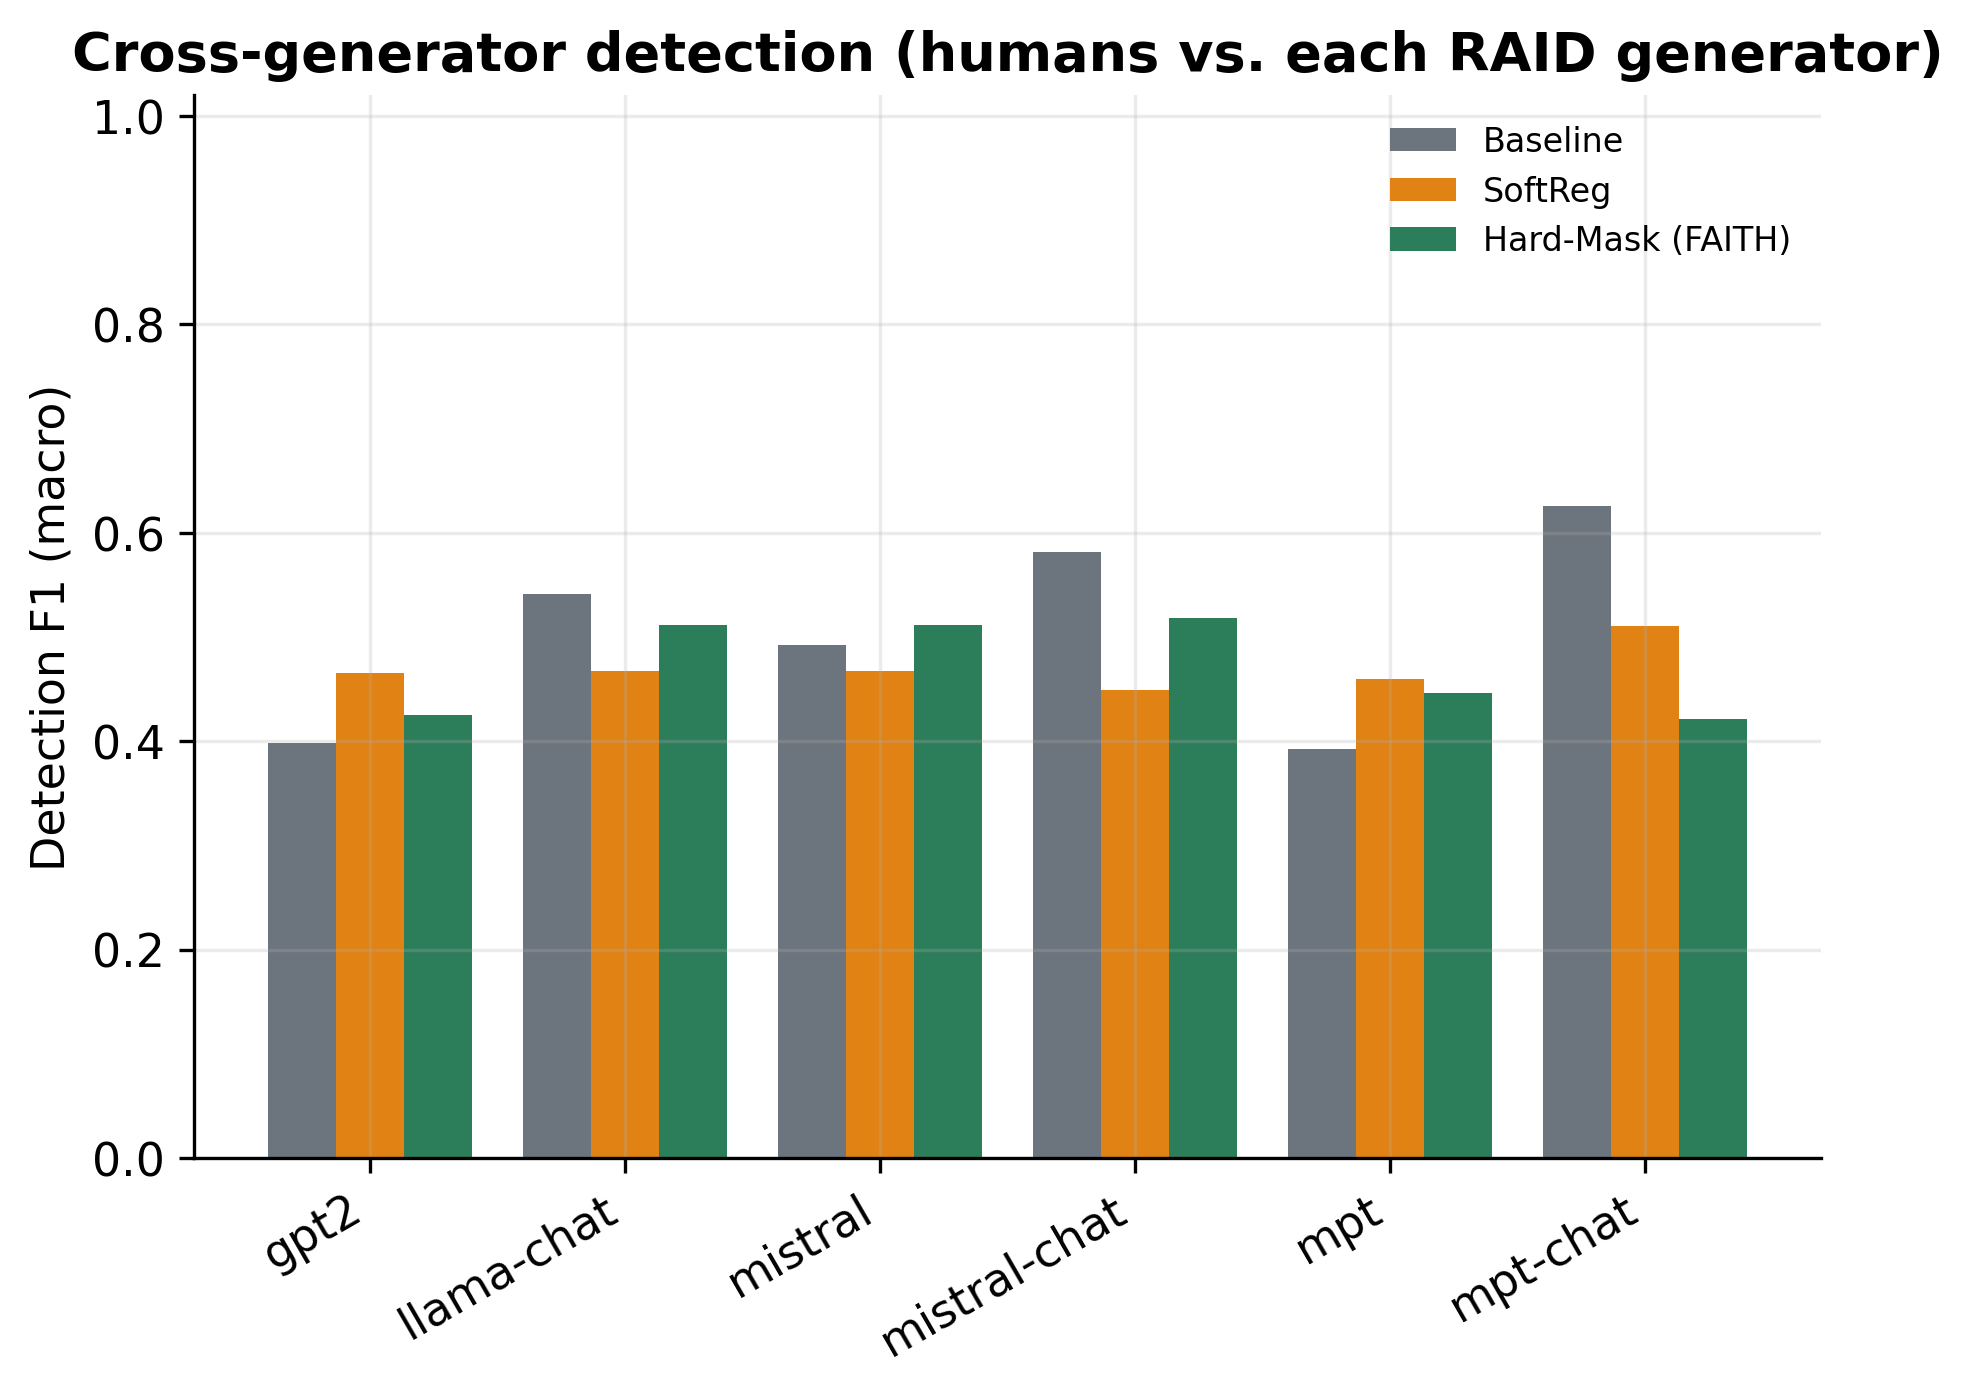
\includegraphics[width=\textwidth]{figures/06b_cross_generator.png}
\caption{Per-generator detection F1 on RAID reviews.}
\label{fig:06b_cross_generator}
\end{figure*}
\paragraph{Why the transfer fails: attribution carry-over.}
To see the mechanism rather than infer it, we attribute the hard-masked model's decisions directly and ask where its evidence lives. In-domain, the model concentrates: 50\% of its attribution mass falls on its 50 most-attributed in-domain content words. Out of domain, that same vocabulary receives only 3\% of the attribution---the content words the model learned to trust are simply absent from the new text. Accuracy tracks this collapse exactly: 90\% in-domain versus 55\% OOD on the diagnostic sample (Figure~\ref{fig:15_ood_diagnostic_hardmask}). Concretely, the model has not learned a transferable notion of ``machine-written''; it has learned a domain-specific content lexicon that does not carry over. This favours a \emph{data} explanation (the training domain fixed the vocabulary the model could use) over a purely \emph{structural} one (invariance dooming transfer in principle), and it is the direct motivation for the mixed-generator experiment that follows.
\begin{figure*}[tp]\centering
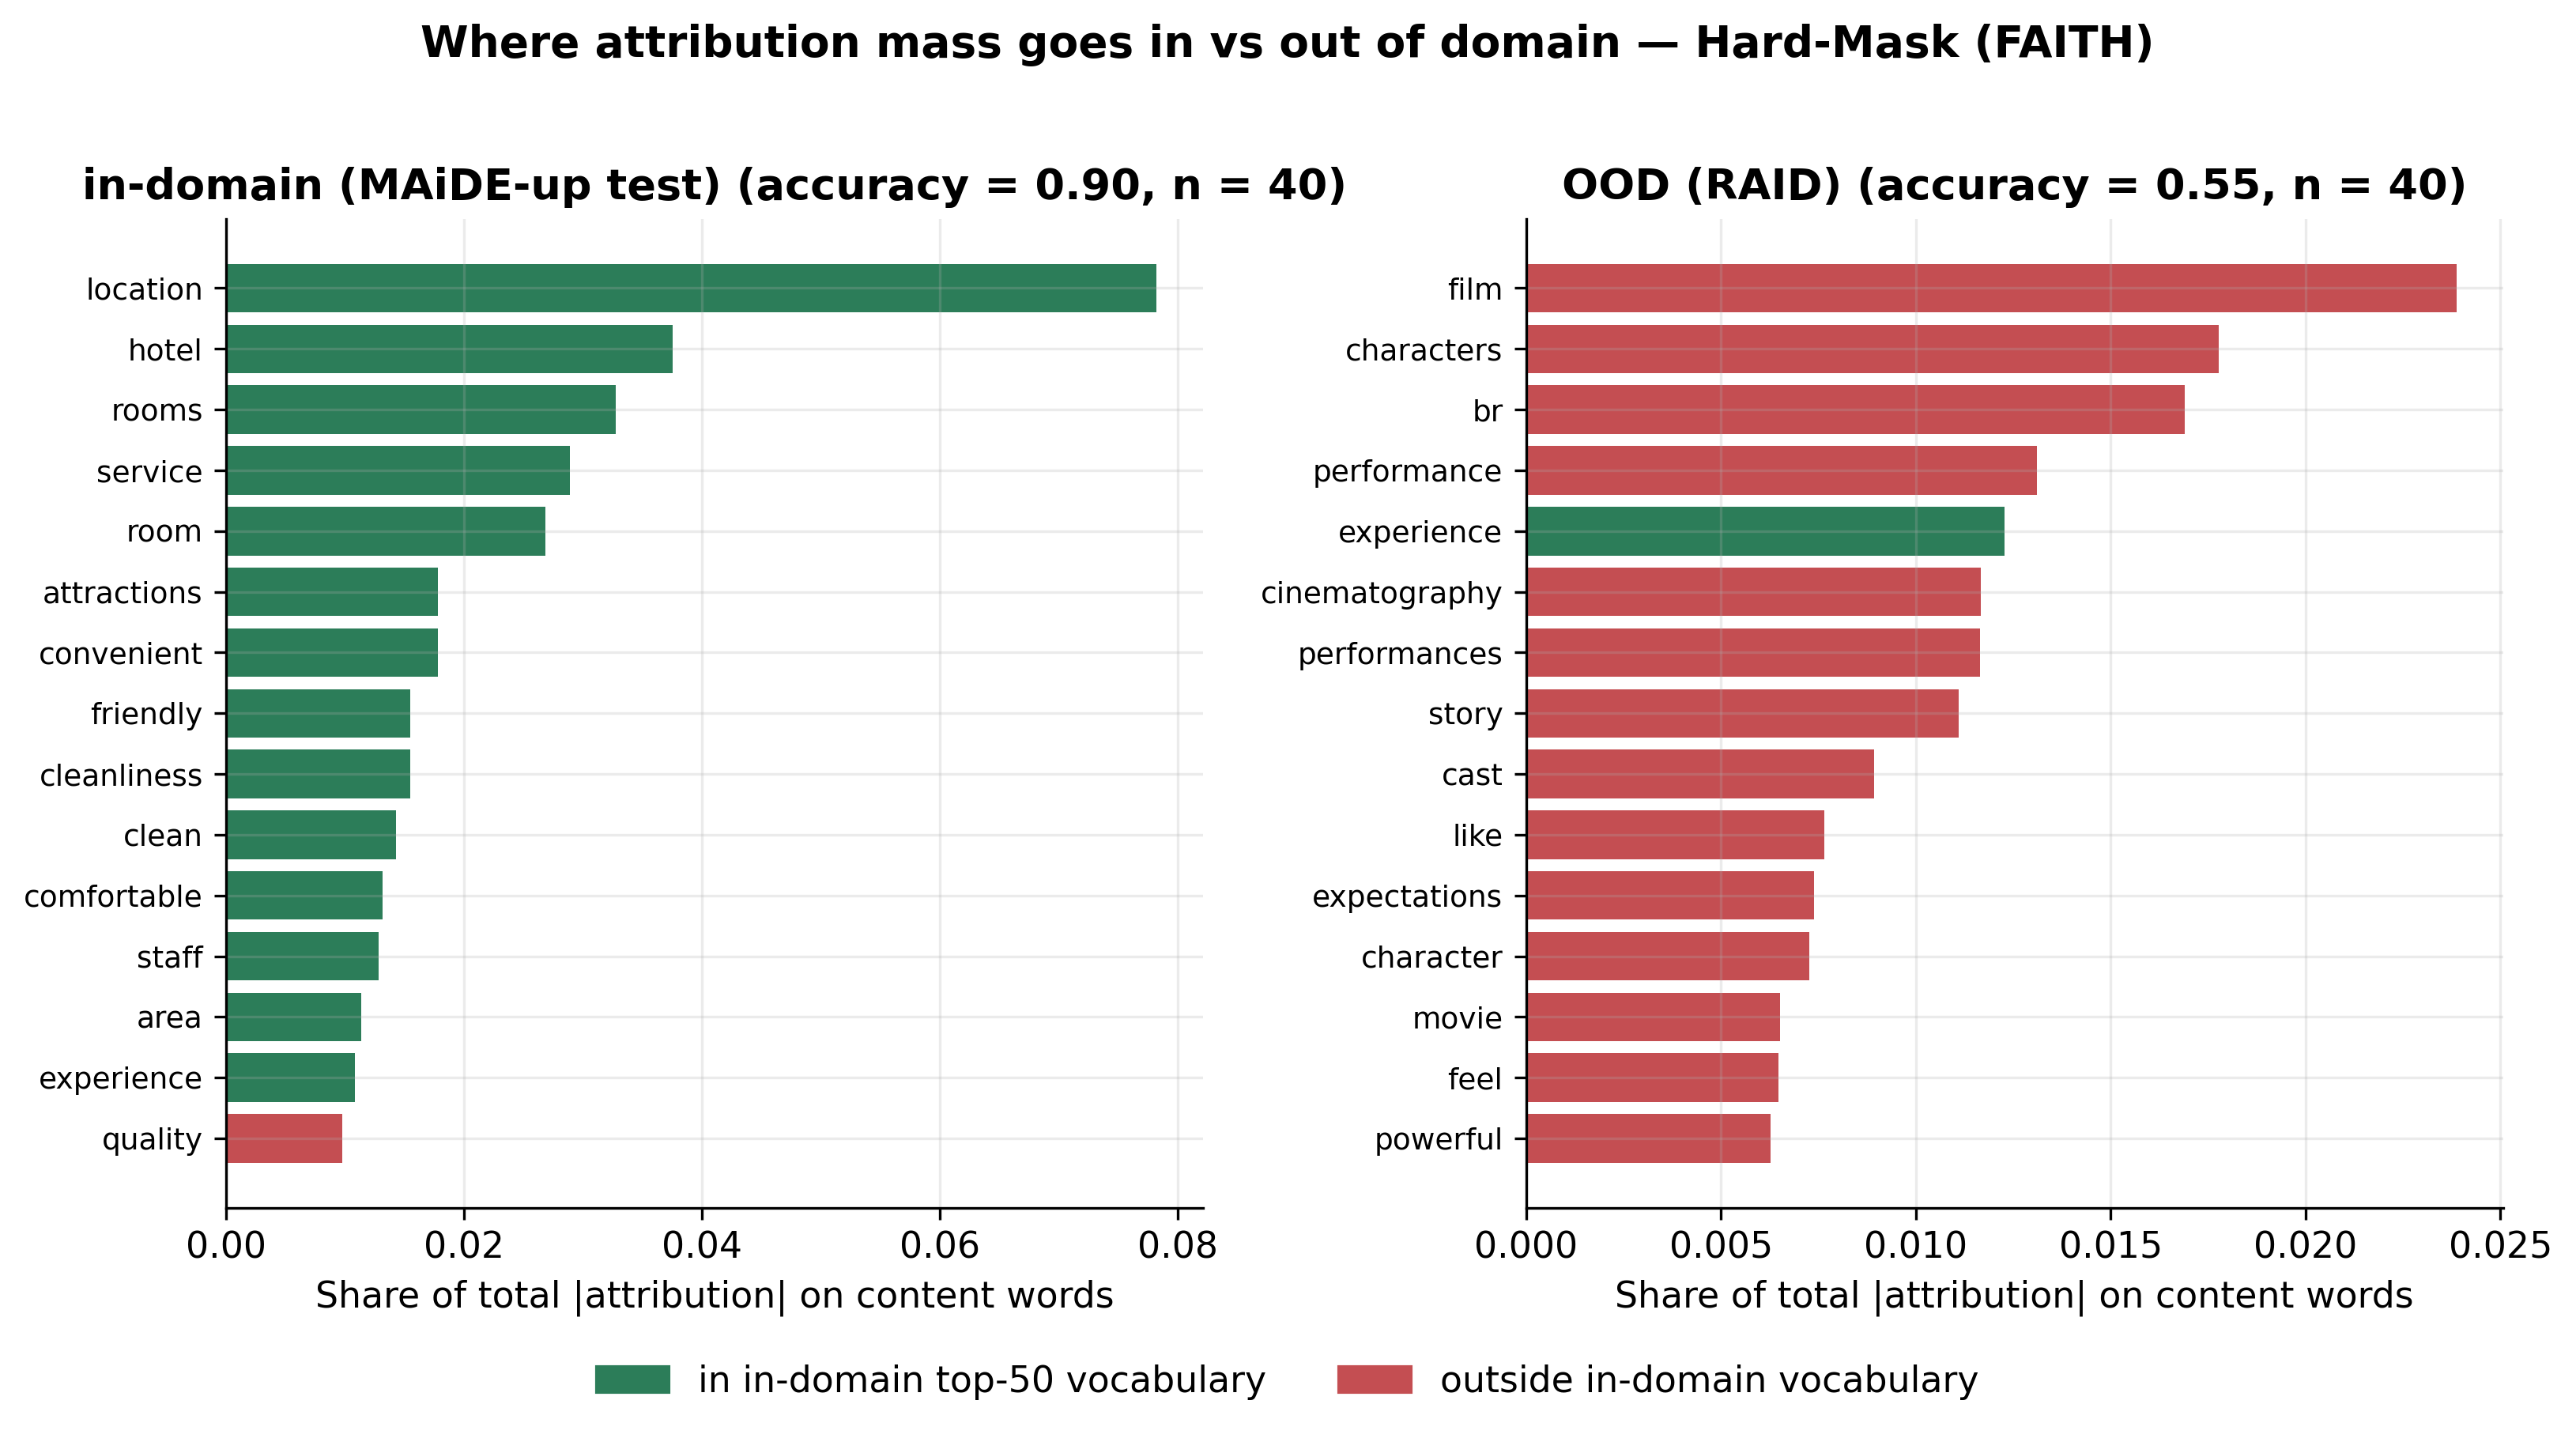
\includegraphics[width=\textwidth]{figures/15_ood_diagnostic_hardmask.png}
\caption{Top-attributed content words for the Hard-Mask model, in-domain vs.\ OOD.}
\label{fig:15_ood_diagnostic_hardmask}
\end{figure*}
\subsection{Mixed-generator training and held-out generators}\label{sec:mixedgen}
The previous OOD test entangles domain shift and generator shift. Here we untangle them. The goal is to hold the domain fixed and vary only the generator, so that whatever gap remains can be attributed to the generator change (and to the invariance constraint) rather than to a change of subject matter.

Concretely, we keep everything in the reviews domain and split by generator. We add same-domain reviews from a set of \emph{held-in} generators (llama-chat, mistral, mpt-chat, cohere, plus half of the human reviews) to the training set, and we evaluate on a disjoint frame of \emph{held-out} generators (gpt3, gpt2, mistral-chat, mpt, plus the remaining humans). Because both train and test now sit in the same domain, the held-out-generator evaluation is same-domain, different-generator by construction---the clean test the OOD set could not provide. This is run at pilot scale (distilroberta-base, 5 seeds, a 600-review training subsample), so we read it for direction rather than precise magnitudes.
\begin{table}[tb]\centering
\caption{Mixed-generator training: same-domain transfer to unseen generators (mean $\pm$ 95\% CI; \% units).}
\label{tab:mixedgen}
\footnotesize
\begin{tabular}{lcc}
\toprule
Variant & In-domain F1 & \shortstack{Held-out-generator\\F1 (same domain)} \\
\midrule
Baseline & 93.0 $\pm$ 2.0 & 85.5 $\pm$ 3.6 \\
SoftReg & 92.1 $\pm$ 2.0 & 85.4 $\pm$ 2.8 \\
Hard-Mask (FAITH) & 91.6 $\pm$ 2.2 & 81.6 $\pm$ 1.0 \\
\bottomrule
\end{tabular}
\end{table}
The result is informative. Even with generator-diverse training data and the domain held fixed, the baseline keeps a roughly 4-point advantage over Hard-Mask on unseen generators (Figure~\ref{fig:06c_heldout_generator}). Because the domain no longer changes, this residual gap cannot be blamed on vocabulary shift alone. Part of the transfer cost is therefore attributable to the invariance constraint itself: discarding function words removes style cues that help recognise an unseen generator. The gap is far smaller than in the cross-domain setting, however, which reinforces the reading from the previous subsection---domain shift is the larger problem, and the invariance penalty is real but secondary.
\begin{figure*}[tp]\centering
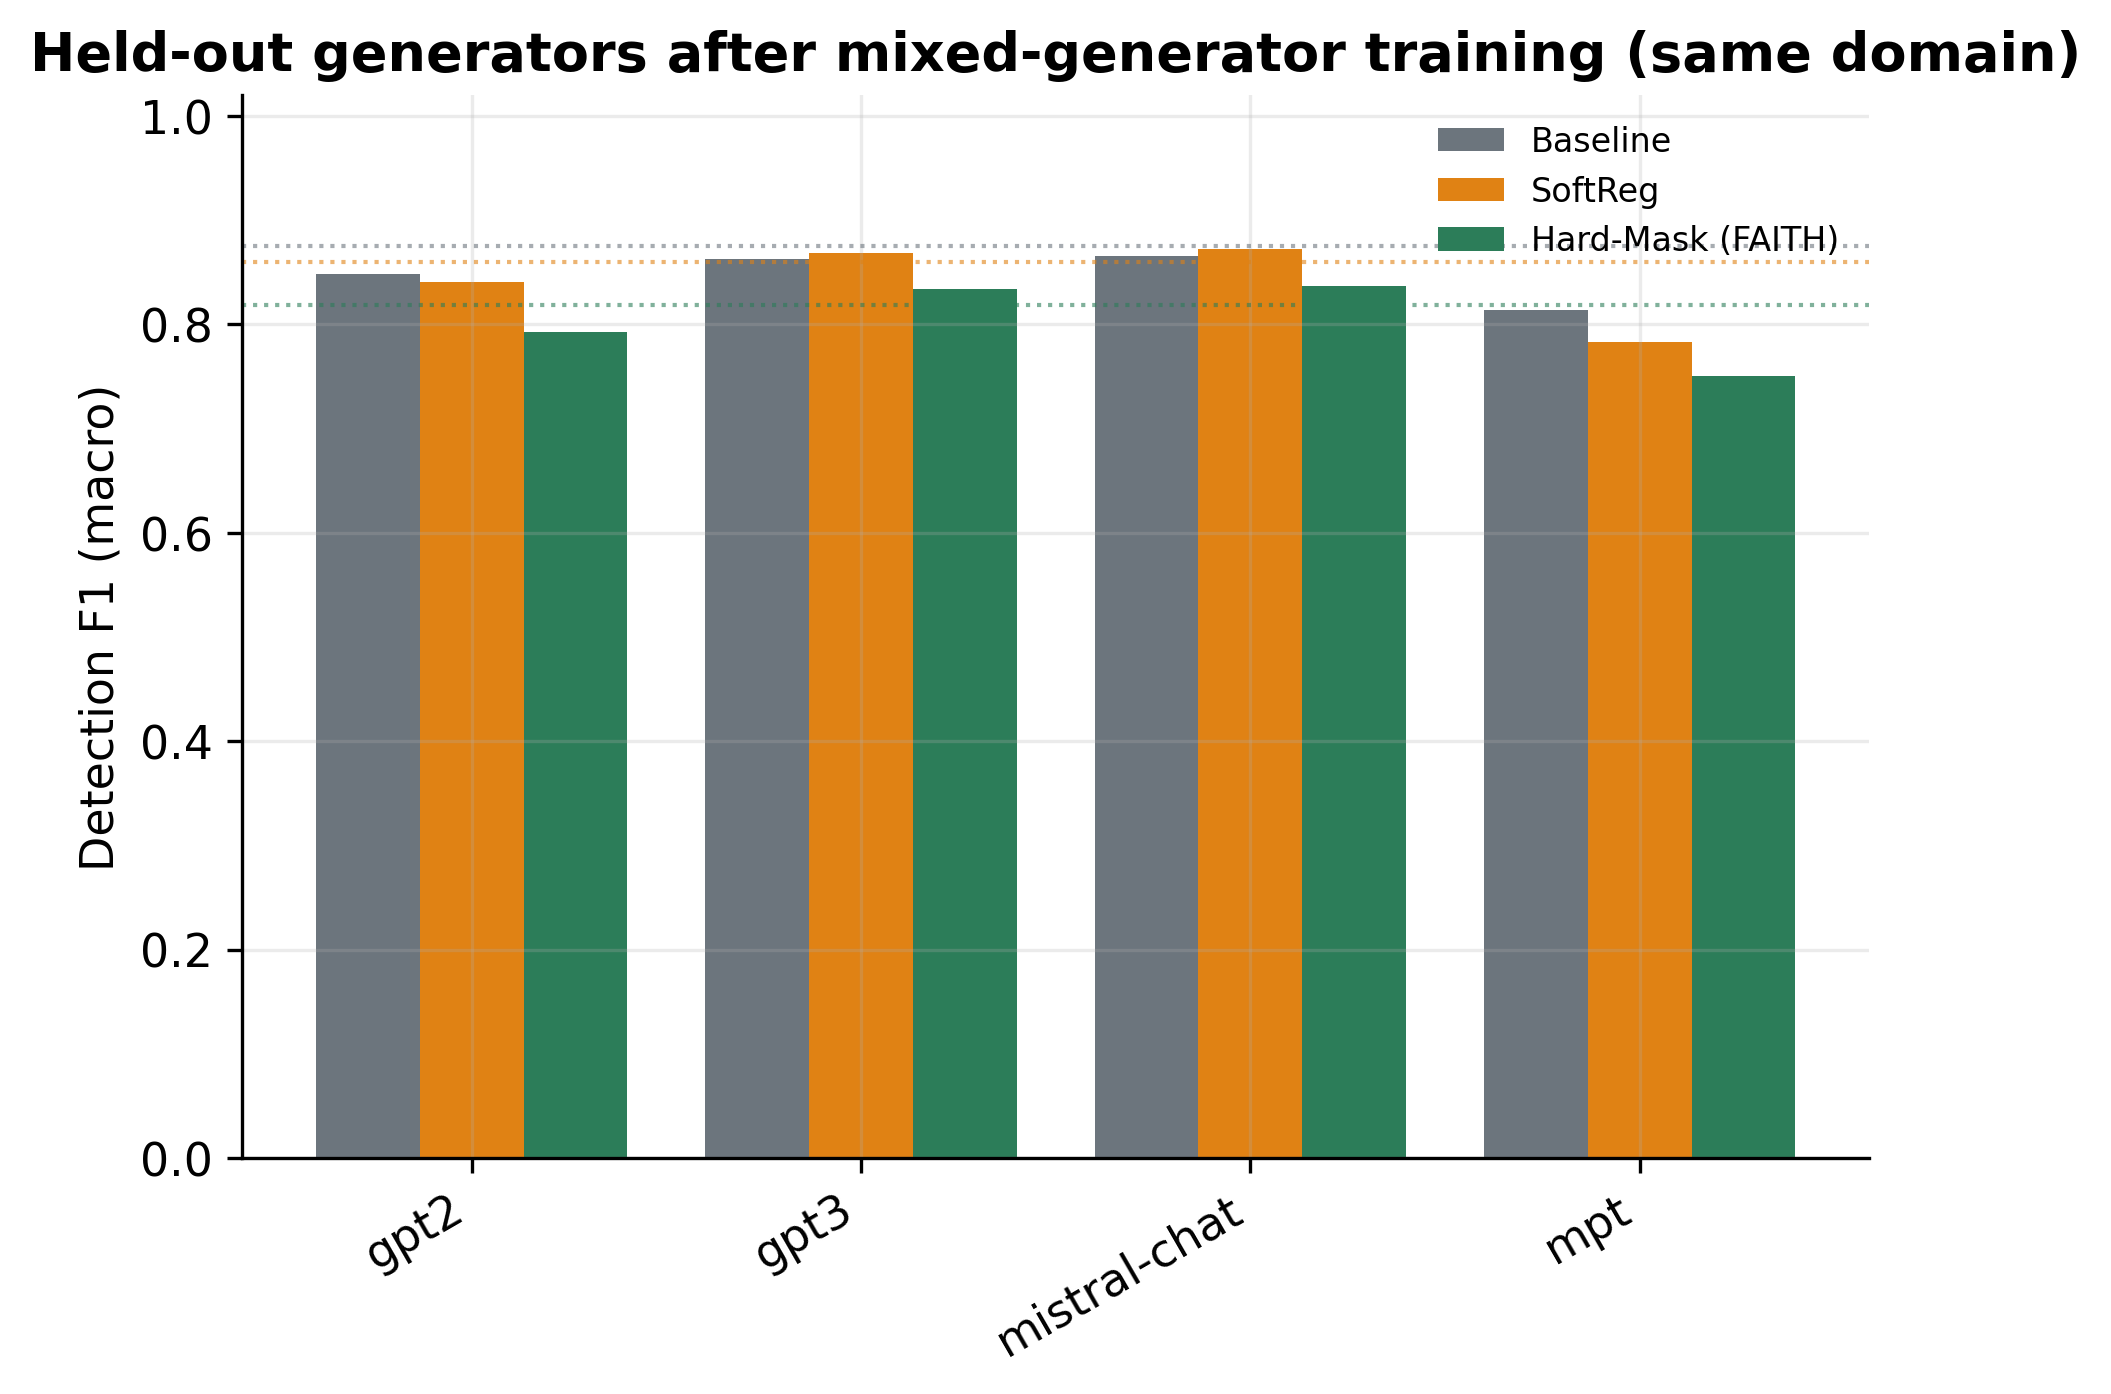
\includegraphics[width=\textwidth]{figures/06c_heldout_generator.png}
\caption{Held-out generators after mixed-generator training (same domain).}
\label{fig:06c_heldout_generator}
\end{figure*}
\subsection{Which function words carry the signal? A per-category ablation}\label{sec:catablation}
If function words carry domain-general style signal, a natural follow-up is to ask \emph{which} function words matter most. We answer it by ablation. Instead of masking the whole function-word set at once, we retrain the hard-masked detector masking exactly one grammatical category at a time---determiners, pronouns, prepositions, conjunctions, auxiliaries, or adverbial function words---while leaving the others visible. The full union mask (every category hidden) is included as the reference upper bound on removal. The logic is that the more transfer drops when a category is hidden, the more that category was contributing to transferable signal. As above, this runs at pilot scale (distilroberta-base, 5 seeds, a 600-review training subsample).
\begin{table}[tb]\centering
\caption{Masking one function-word category at a time (Hard-Mask variant).}
\label{tab:catab}
\footnotesize
\begin{tabular}{lcc}
\toprule
Masked category & In-domain F1 & OOD F1 \\
\midrule
mask adverbial & 93.0 $\pm$ 1.1 & 46.1 $\pm$ 12.6 \\
mask auxiliaries & 92.7 $\pm$ 2.1 & 45.1 $\pm$ 7.8 \\
mask conjunctions & 91.7 $\pm$ 2.8 & 47.2 $\pm$ 12.4 \\
mask determiners & 93.5 $\pm$ 1.1 & 46.5 $\pm$ 6.8 \\
mask prepositions & 93.2 $\pm$ 1.4 & 50.3 $\pm$ 4.9 \\
mask pronouns & 93.1 $\pm$ 0.8 & 48.9 $\pm$ 7.5 \\
mask union & 89.8 $\pm$ 3.7 & 35.3 $\pm$ 2.8 \\
\bottomrule
\end{tabular}
\end{table}
Two patterns stand out. First, in-domain F1 is barely touched by hiding any single category, confirming that no one category is load-bearing in distribution. Second, the categories separate on transfer: masking \emph{auxiliaries} gives the lowest OOD F1 (45\%) and masking \emph{prepositions} the highest (50\%), with the full union mask far below either (35\%) (Figure~\ref{fig:16_category_ablation}). The reading is that auxiliaries carry comparatively more of the transferable style signal than prepositions do. We treat this ordering as suggestive rather than conclusive, given the pilot scale and the overlapping intervals, and we release the protocol so it can be replicated at full scale.
\begin{figure*}[tp]\centering
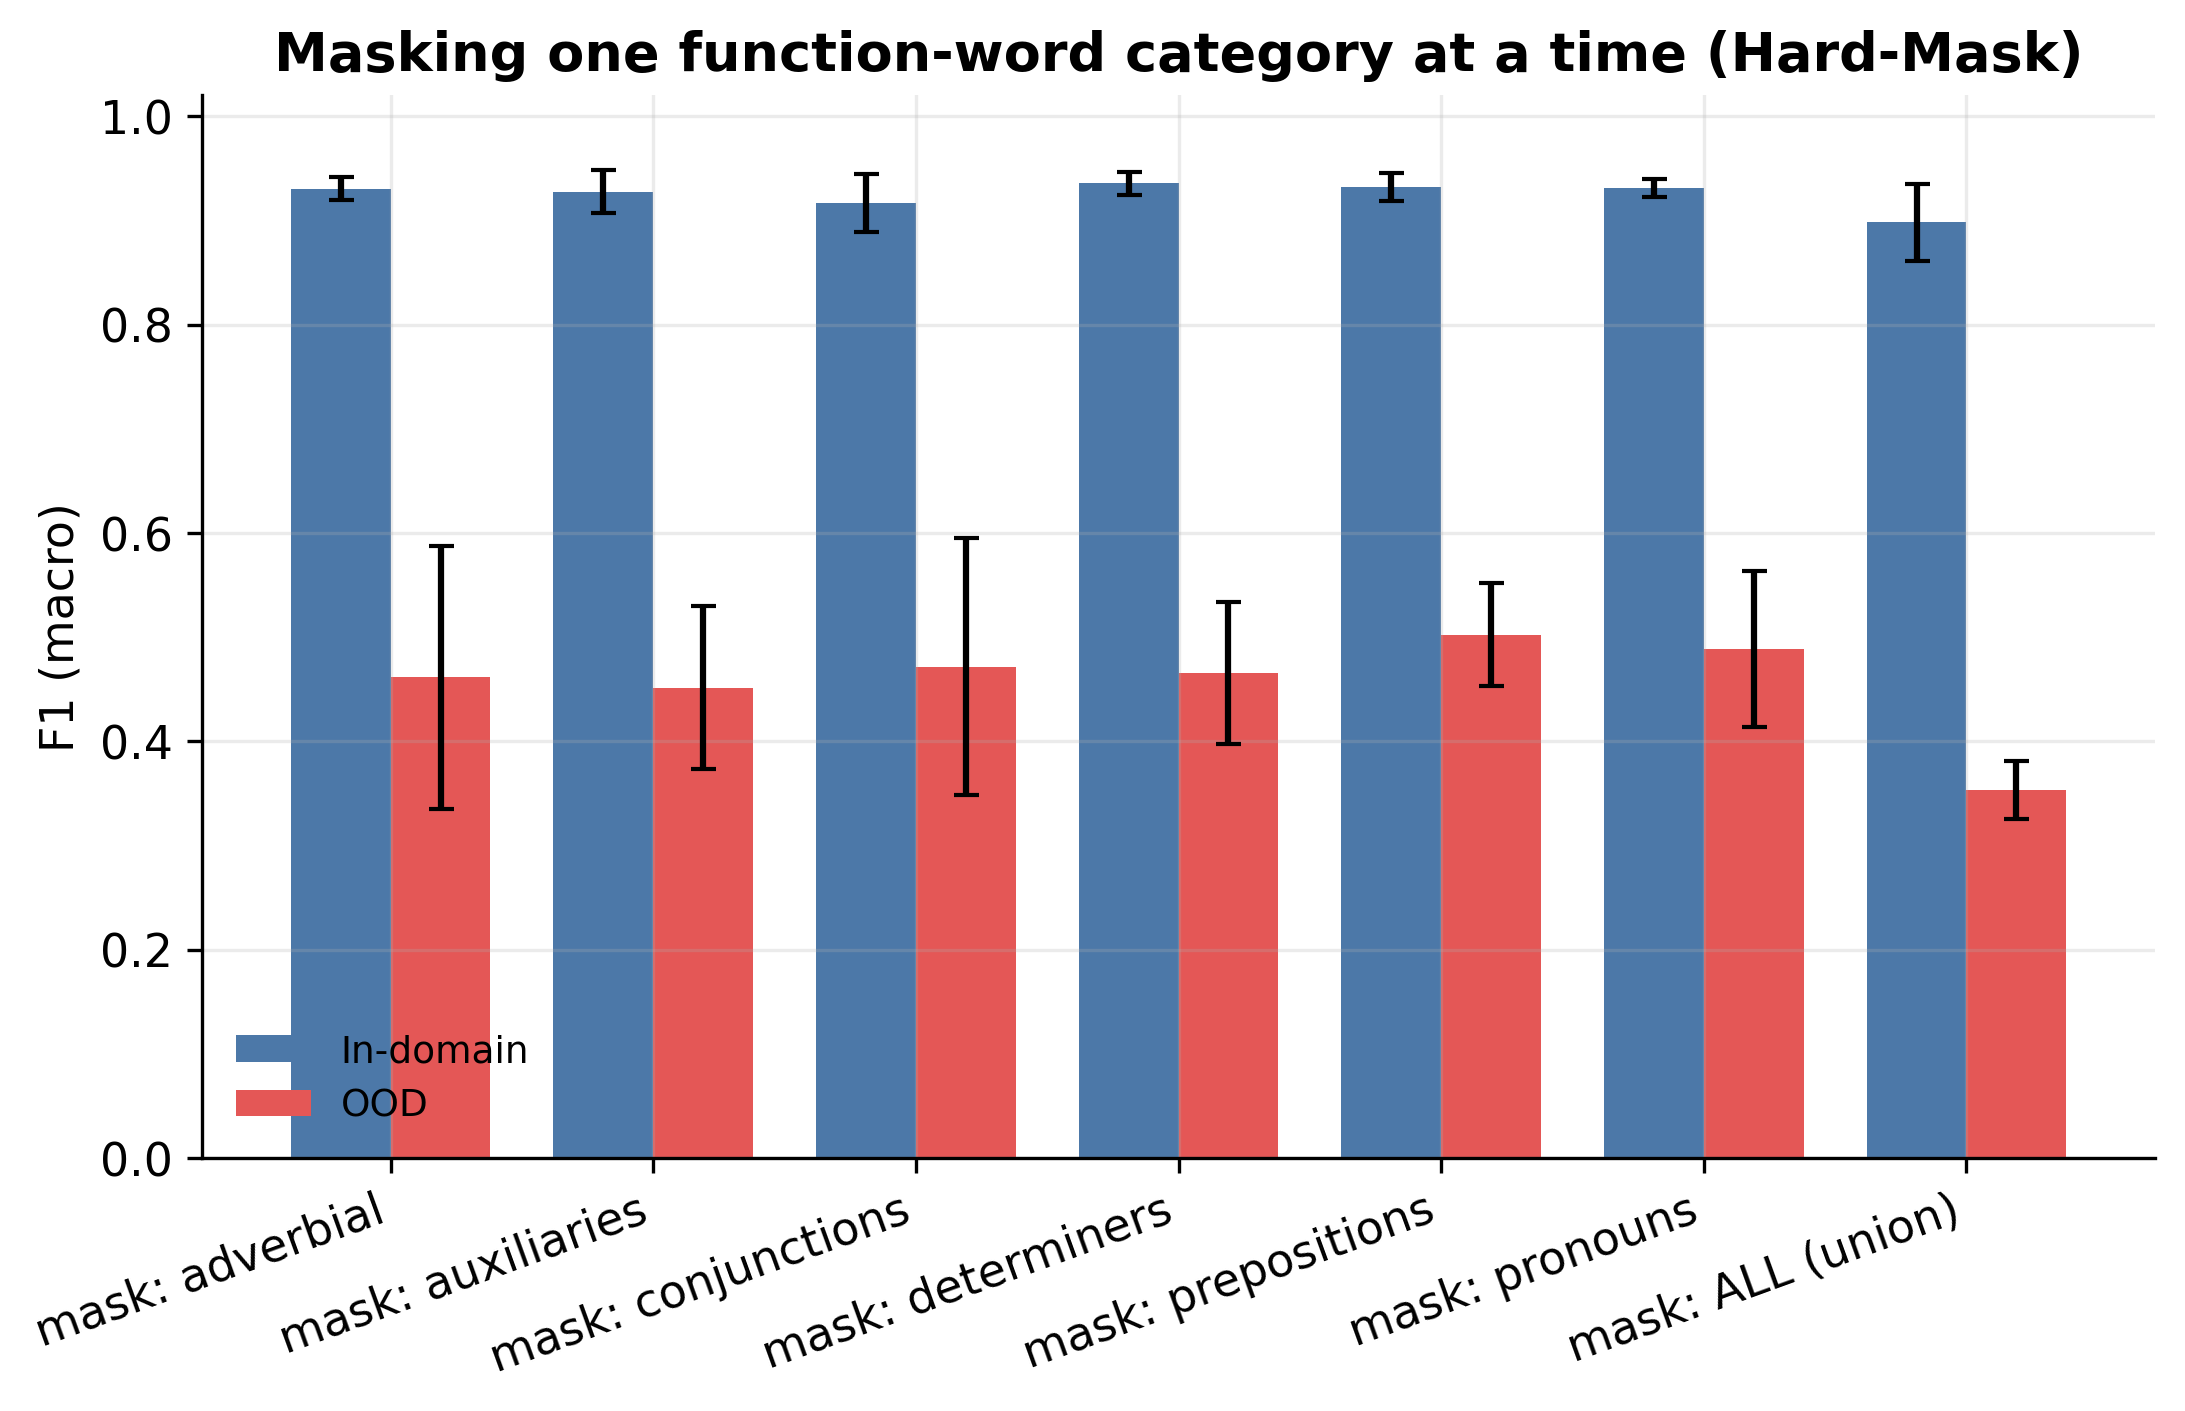
\includegraphics[width=\textwidth]{figures/16_category_ablation.png}
\caption{Per-category masking ablation: in-domain vs.\ OOD F1.}
\label{fig:16_category_ablation}
\end{figure*}
\subsection{Identity, slot, or position? A masking-variant comparison}\label{sec:variantcmp}
The slot-reliance result (\S\ref{sec:faith}, Table~\ref{tab:slotmass}) showed that hard masking removes function-word identity but not the slots. To separate \emph{which} aspect of function words carries signal---their identity, the consistent slot-marker, or the bare positions and counts---we train four detectors that remove function-word information in increasingly aggressive ways and compare them head to head. \textbf{Baseline} keeps everything. \textbf{Hard-Mask} replaces each function word with a single shared \texttt{[FUNC]} token: identity is erased but the slot (a consistent marker, at its original position) remains. \textbf{Random} replaces each function word with a fresh random token: identity \emph{and} the consistent marker are gone, but the perturbed positions and counts remain. \textbf{Deletion} drops function words entirely: identity, marker and the original positions all disappear. Table~\ref{tab:variantcmp} and Figure~\ref{fig:variantcmp} report the comparison (pilot: distilroberta-base, seed 0).

\begin{table}[tb]\centering
\caption{Masking-variant comparison (pilot: distilroberta-base, seed 0; macro F1 \%). Every route that removes function-word information keeps in-domain accuracy but loses cross-domain F1.}
\label{tab:variantcmp}
\footnotesize
\begin{tabular}{lcc}
\toprule
Variant & In-domain F1 & OOD F1 \\
\midrule
Baseline (keeps everything) & 93.7 & 50.3 \\
Hard-Mask (\texttt{[FUNC]}; slot kept) & 89.2 & 37.0 \\
Random (identity + marker gone) & 91.2 & 38.8 \\
Deletion (function words removed) & 94.0 & 33.3 \\
\bottomrule
\end{tabular}
\end{table}

\begin{figure}[tb]\centering
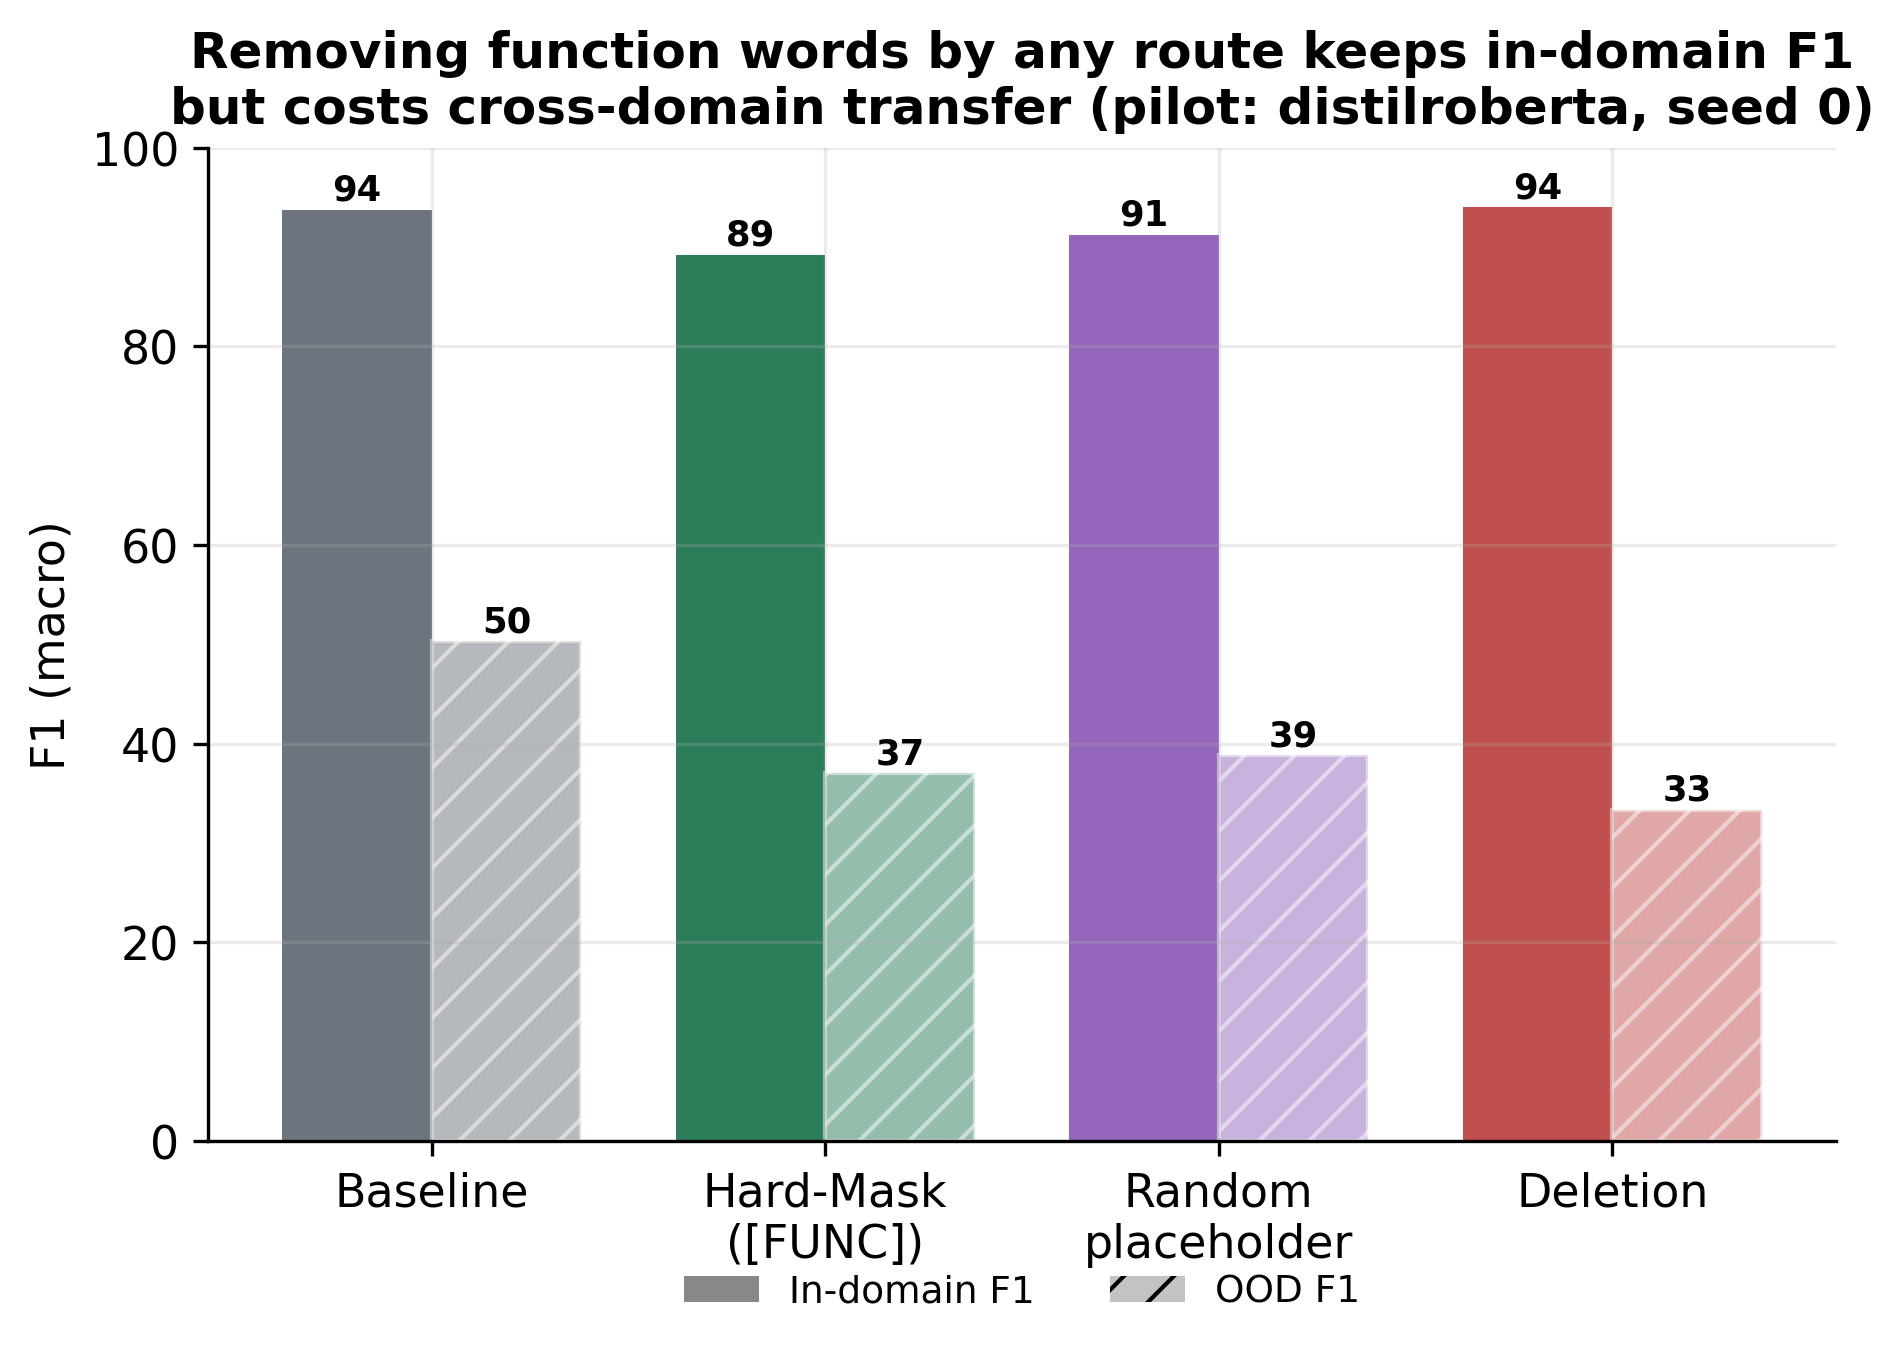
\includegraphics[width=\linewidth]{figures/variant_comparison.png}
\caption{Masking-variant comparison. In-domain F1 is preserved by every variant (89--94); cross-domain F1 falls for all of them (33--39 vs.\ 50 for the baseline), regardless of how the function words are removed.}
\label{fig:variantcmp}
\end{figure}

Two findings emerge, and we state them with single-seed caution. First, removing function-word information is essentially free \emph{in distribution}: all three constrained variants stay within a few points of the baseline (89--94 F1), and deletion even matches it (94.0). So the in-domain task does not need function words by any definition. Second, all three constrained variants lose cross-domain F1 by a similar margin (37.0/38.8/33.3 vs.\ the baseline's 50.3), and the differences \emph{among} them are small relative to the gap from the baseline. The transferable signal that function words carry is therefore not pinned to one specific property: erasing identity already costs most of it, and additionally removing the slot-marker (Random) or the positions (Deletion) does not change the picture qualitatively. If anything, deletion---which destroys the most structure---transfers worst, consistent with positions and counts carrying a little residual domain-general signal on top of identity. We treat the fine ordering as suggestive only (one seed) and release the variants and protocol for full-scale replication.

\subsection{How much does the SoftReg penalty weight matter?}\label{sec:lambda}
The soft variant is governed by a single knob, the penalty weight $\lambda$ in Eq.~\ref{eq:softreg}. A reviewer might reasonably ask whether a stronger penalty trades function-word reliance for accuracy along a useful frontier. We sweep $\lambda \in \{0, 0.25, 0.5, 1, 2, 4\}$ at full scale (\texttt{roberta-base}, full MAiDE-up, 3 seeds; $\lambda{=}0$ recovers the baseline) and report in-domain F1 and the forward-only identity-sensitivity at each setting (Table~\ref{tab:lambda}, Figure~\ref{fig:lambda}).

\begin{table}[tb]\centering
\caption{SoftReg penalty sweep (roberta-base, full data, 3 seeds). In-domain F1 with 95\% CI; identity-sensitivity as a point estimate (its 3-seed intervals are wide---$\pm10$ to $\pm21$---and mutually overlapping, so we do not read a trend into them).}
\label{tab:lambda}
\footnotesize
\begin{tabular}{lcc}
\toprule
$\lambda$ & In-domain F1 & Identity-sens.\ $|\Delta p|$ \\
\midrule
0.0 & 95.8 $\pm$ 2.6 & 5.1\% \\
0.25 & 94.5 $\pm$ 4.4 & 8.1\% \\
0.5 & 94.7 $\pm$ 4.4 & 9.2\% \\
1.0 & 94.7 $\pm$ 4.7 & 9.2\% \\
2.0 & 94.8 $\pm$ 4.0 & 6.7\% \\
4.0 & 84.3 $\pm$ 17.0 & 12.7\% \\
\bottomrule
\end{tabular}
\end{table}

\begin{figure}[tb]\centering
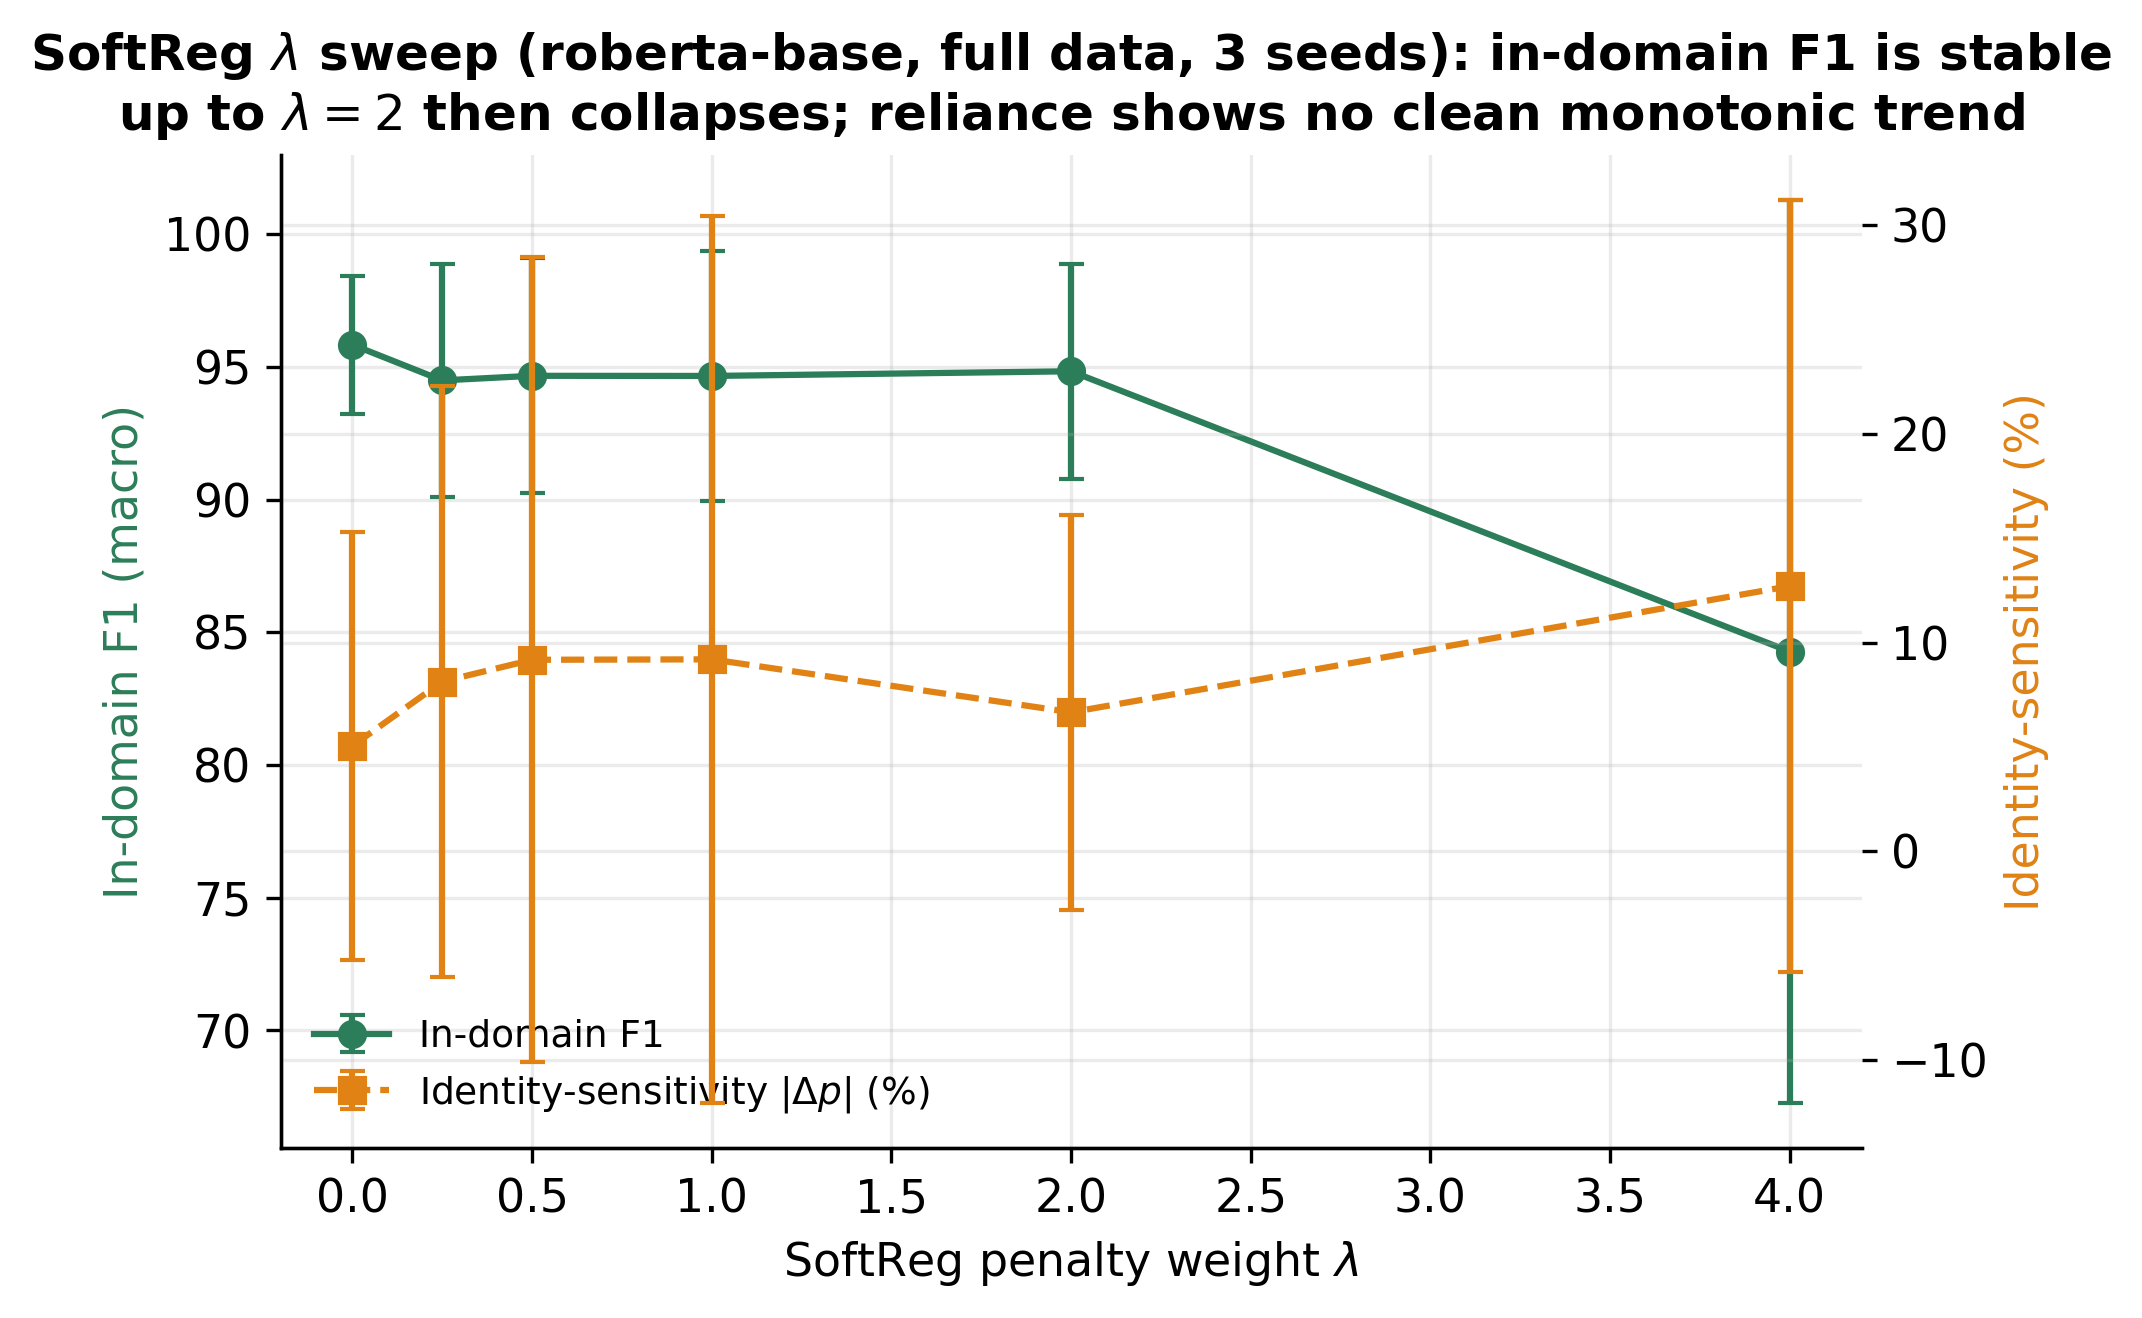
\includegraphics[width=\linewidth]{figures/lambda_sweep.png}
\caption{SoftReg penalty sweep. In-domain F1 is flat across $\lambda\in[0,2]$ and collapses at $\lambda{=}4$; the measured function-word reliance (identity-sensitivity) shows no clean monotonic trend, and its 3-seed intervals are wide.}
\label{fig:lambda}
\end{figure}

The result is informative precisely because it is negative. In-domain accuracy is insensitive to $\lambda$ across two orders of magnitude ($\sim$95 F1 for $\lambda \le 2$) and then collapses once the penalty dominates the cross-entropy ($84.3$ at $\lambda{=}4$). Crucially, the penalty does \emph{not} buy a clean reduction in measured reliance: identity-sensitivity wanders between $5$ and $13\%$ with no monotonic relationship to $\lambda$, and the 3-seed intervals are too wide to support any ordering. In other words, the soft penalty is not a dependable reliance--accuracy dial---it leaves accuracy untouched until it breaks it, without demonstrably moving reliance in between. This reinforces the paper's central contrast: if the goal is a \emph{guaranteed} bound on function-word-identity reliance, hard masking provides it by construction, whereas tuning the soft penalty does not reliably deliver it.

\subsection{Few-shot domain recovery}\label{sec:fewshot}
The attribution diagnostic argued that the cross-domain failure is mostly a missing-vocabulary problem rather than a structural ceiling. If that is right, then a small amount of labelled target-domain data should recover a large share of the lost accuracy. We test this directly. We take the hotel-trained Hard-Mask model, fine-tune it on $k$ labelled out-of-domain reviews, and evaluate on a fixed held-out OOD test set, sweeping $k$ from 0 (no adaptation) upward.
\begin{table}[tb]\centering
\caption{Few-shot domain adaptation of the Hard-Mask model (mean $\pm$ 95\% CI over few-shot samples).}
\label{tab:fewshot}
\footnotesize
\begin{tabular}{lc}
\toprule
Labelled OOD examples $k$ & OOD F1 \\
\midrule
0 & 34.3 $\pm$ 0.0 \\
50 & 47.3 $\pm$ 14.0 \\
100 & 58.6 $\pm$ 20.9 \\
200 & 77.2 $\pm$ 1.5 \\
\bottomrule
\end{tabular}
\end{table}
The recovery is steep. Moving from $k=0$ to $k=200$ labelled examples lifts OOD F1 from 34\% to 77\%---a gain of more than 40 points from only a couple of hundred labelled reviews. This is the strongest evidence that the cross-domain gap is largely a labelled-data requirement, not a structural limitation of the invariant detector: when the model is shown even a little of the target vocabulary, most of the deficit closes. Practically, it reframes the trade-off. Hard masking does not permanently forfeit transfer; it forfeits \emph{zero-shot} transfer, and a modest, realistic amount of target-domain labelling restores much of the loss.

\subsection{Which function words carry the signal? Word-level statistics}
A per-category ablation tells us \emph{which kinds} of function words matter, but not which individual words. To answer that, we move from the model to the corpus itself and measure how each function word is distributed across the two classes. The tool is the Monroe et al.\ ``Fightin' Words'' log-odds ratio with an informative Dirichlet prior. In plain terms, this is a smoothed comparison of how much more often a word appears in AI text than in human text, expressed as a $z$-score whose magnitude reflects how confident we can be that the difference is real rather than a sampling fluke. We compute this statistic for every function word in-domain, contrasting AI and human reviews. We then repeat the identical computation on the out-of-domain reviews pool. The second pass is the important one: it lets us test the \emph{stability} of each signal, that is, whether a word that leans AI in hotels still leans AI in the new domain.

\begin{table}[tb]\centering
\caption{Strongest function-word signals and their cross-domain stability.}
\label{tab:fwstats}
\footnotesize
\begin{tabular}{lccc}
\toprule
Function word & $z$ (in-domain) & $z$ (OOD) & Sign stable? \\
\midrule
the & +16.5 & -6.5 & \textbf{flips} \\
we & -13.8 & -12.7 & yes \\
i & -12.8 & -48.2 & yes \\
no & -10.4 & -13.6 & yes \\
you & -10.2 & -12.1 & yes \\
that & -9.1 & +29.0 & \textbf{flips} \\
they & -9.1 & -3.2 & yes \\
was & +9.1 & -20.1 & \textbf{flips} \\
\bottomrule
\end{tabular}
\end{table}

The headline number is instability. Across all significant ($|z|>2$) function-word signals, only 69\% keep their sign when the domain changes; the remaining third actually reverse direction. The clearest example is the article ``the''. In hotel reviews it is the strongest AI-leaning signal of any function word, yet out-of-domain it flips and leans human instead. The pronouns behave very differently: humans write ``I'' and ``we'' more than the model in \emph{every} domain, so these signals are stable and form a reliable family (Figure~\ref{fig:17_fw_words}). In short, some function-word cues are genuinely cross-domain (the personal pronouns) while others, including the single most frequent word in English, are tied to the corpus that produced them. This is the word-level statistical basis of our shortcut claim: a large share of the function-word signal that an unconstrained detector absorbs is domain-local, so a model that leans on it learns something that does not travel.

\begin{figure*}[tp]\centering
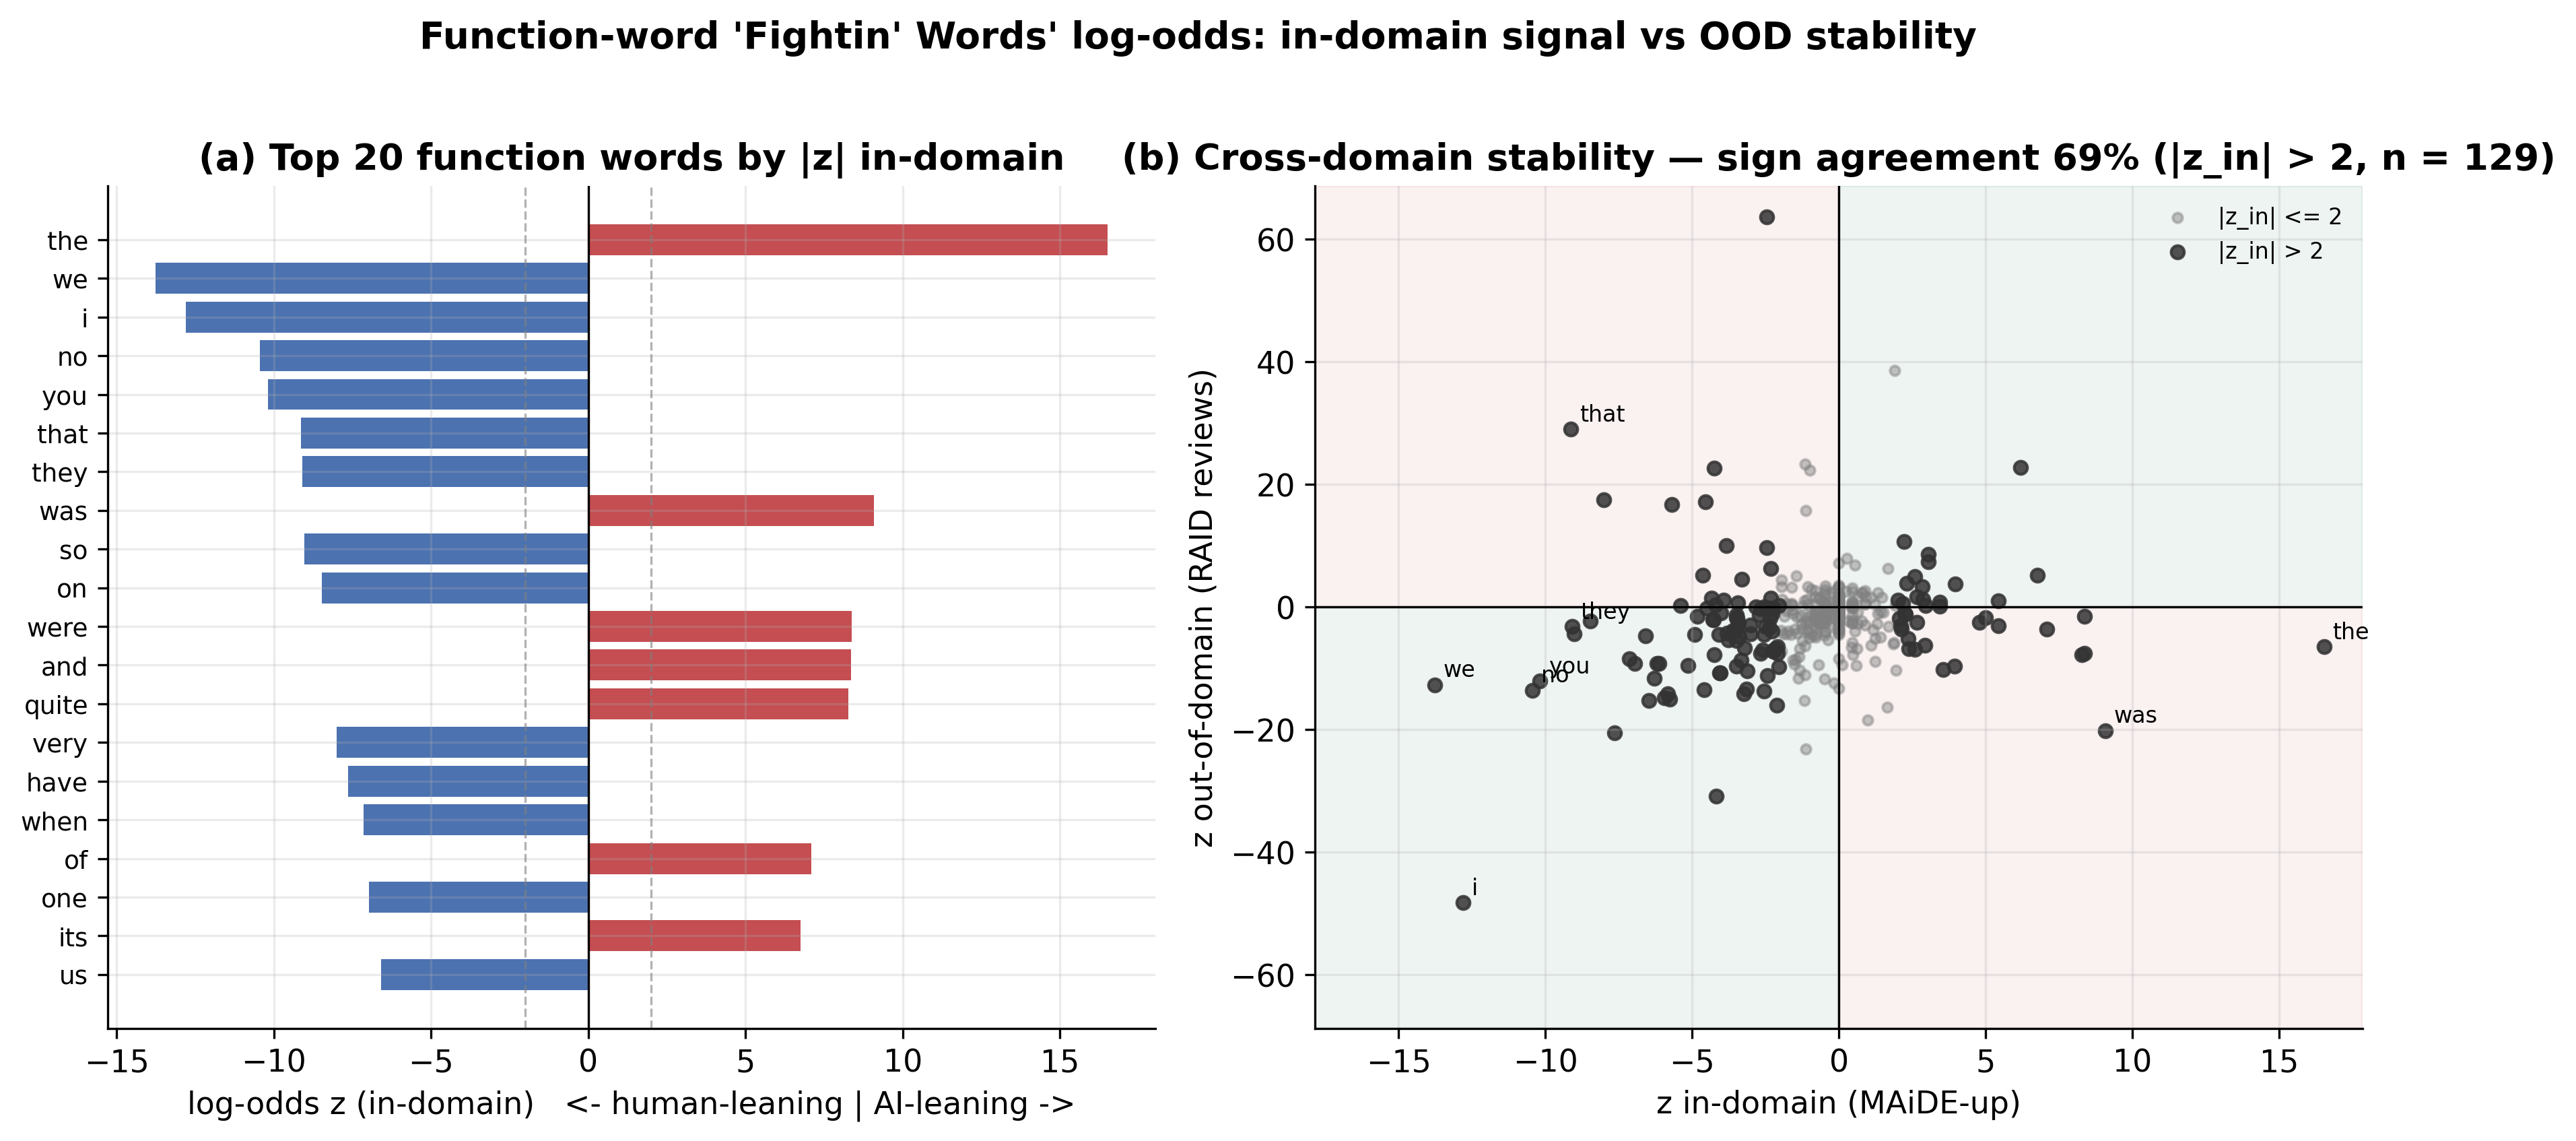
\includegraphics[width=\textwidth]{figures/17_fw_words.png}
\caption{Function-word log-odds: top signals (left) and in-domain vs.\ OOD stability (right).}
\label{fig:17_fw_words}
\end{figure*}

\subsection{Replication on a second corpus (HC3)}
A single in-domain dataset cannot tell us whether our findings are general or an accident of MAiDE-up. We therefore replicate the core comparison on a second, independently collected corpus. HC3 pairs human answers with ChatGPT answers to the same questions. We retrain both the baseline and the Hard-Mask variant from scratch on HC3 and evaluate them three ways: in-corpus, under the function-word attack, and zero-shot transferred to MAiDE-up (so the model never sees a hotel review during training).

\begin{table}[tb]\centering
\caption{Replication on HC3 (pilot: distilroberta-base, $n{=}2$ seeds). In-corpus F1 is at ceiling for both. Transfer is reported \emph{per seed}, not as mean $\pm$ CI: with $n{=}2$ a $t$-interval is uninformative (it yields CIs as wide as $\pm105$ F1 points, an obvious impossibility). Note that ROC-AUC \emph{reverses} the F1 ordering.}
\label{tab:hc3}
\footnotesize
\begin{tabular}{lccc}
\toprule
Variant & In-corpus F1 & \shortstack{$\rightarrow$MAiDE F1\\(per seed)} & \shortstack{$\rightarrow$MAiDE AUROC\\(per seed)} \\
\midrule
Baseline & 100.0 & 57.6 / 41.0 & .835 / .832 \\
Hard-Mask & 100.0 & 66.5 / 60.7 & .692 / .727 \\
\bottomrule
\end{tabular}
\end{table}

\paragraph{Why HC3 reaches ceiling.} Both variants reach (near-)perfect in-corpus F1, which we examined rather than celebrated; a perfect score usually signals that the task is too easy rather than that the model is unusually good. Three factors explain it. First, HC3's ChatGPT-era answers carry blatant register markers --- uniform length, hedging boilerplate, and list-like structure --- and HC3's own release paper documents these as highly separable. (A register marker here is a stylistic regularity tied to how the model was prompted, not to the content of the answer.) Second, our splits are grouped by \emph{question}: HC3 contains several answers per question, and a naive row-level split would leak question context across train and test. We found and removed exactly this hazard, so answers to one question never straddle the boundary, and the ceiling persists even after the fix --- which tells us the easiness is a genuine property of the corpus, not an artefact of leakage. Third, the classifier is fine-tuned on in-corpus data, and ceiling separability under fine-tuning is consistent with prior HC3 results. Taken together, the in-corpus and attack rows certify little beyond corpus easiness; the informative result is the transfer column, and it must be read carefully for two reasons. First, this replication is small: distilroberta-base with only two seeds, so a mean $\pm$ 95\% confidence interval is meaningless here (it produced the absurd $\pm105$ F1 interval we removed), and we report the two per-seed values instead. Second, and more importantly, the two metrics disagree. On macro F1 Hard-Mask transfers \emph{better} than the baseline (mean $63.6$ vs.\ $49.3$); on ROC-AUC the order \emph{reverses} (baseline $\approx0.83$ vs.\ Hard-Mask $\approx0.71$). Because F1 depends on a threshold and AUROC does not, this is the same operating-point sensitivity we saw on RAID, and it means the \emph{sign} of the invariance--transfer effect on HC3 is genuinely undetermined at this scale. We therefore make the weakest claim the data support: a trade-off exists, but neither its sign nor its magnitude is established by this corpus, and a full-scale, multi-seed replication is needed to settle it.

\subsection{Modern open-weight generators}
MAiDE-up's AI half comes from GPT-4, so a fair worry is that the detector has simply memorised one generator's quirks rather than a general signal of machine authorship. To probe this, we generate fresh same-domain hotel reviews with newer models the detector has never seen during training. We use two locally run open-weight LLMs (Llama-3.2-3B and Gemma-2-2B) and Claude (Haiku and Sonnet tiers, accessed via its command-line interface). Every generator is prompted with real hotel names and cities so the new reviews match the original domain. We then evaluate the trained detectors on each generator separately (Figure~\ref{fig:18_new_generators}). GPT-4o and Gemini require API access we do not have, so they remain future work; we flag this so the coverage is read as a representative sample of current open-weight models rather than an exhaustive survey.

\begin{figure}[tb]\centering
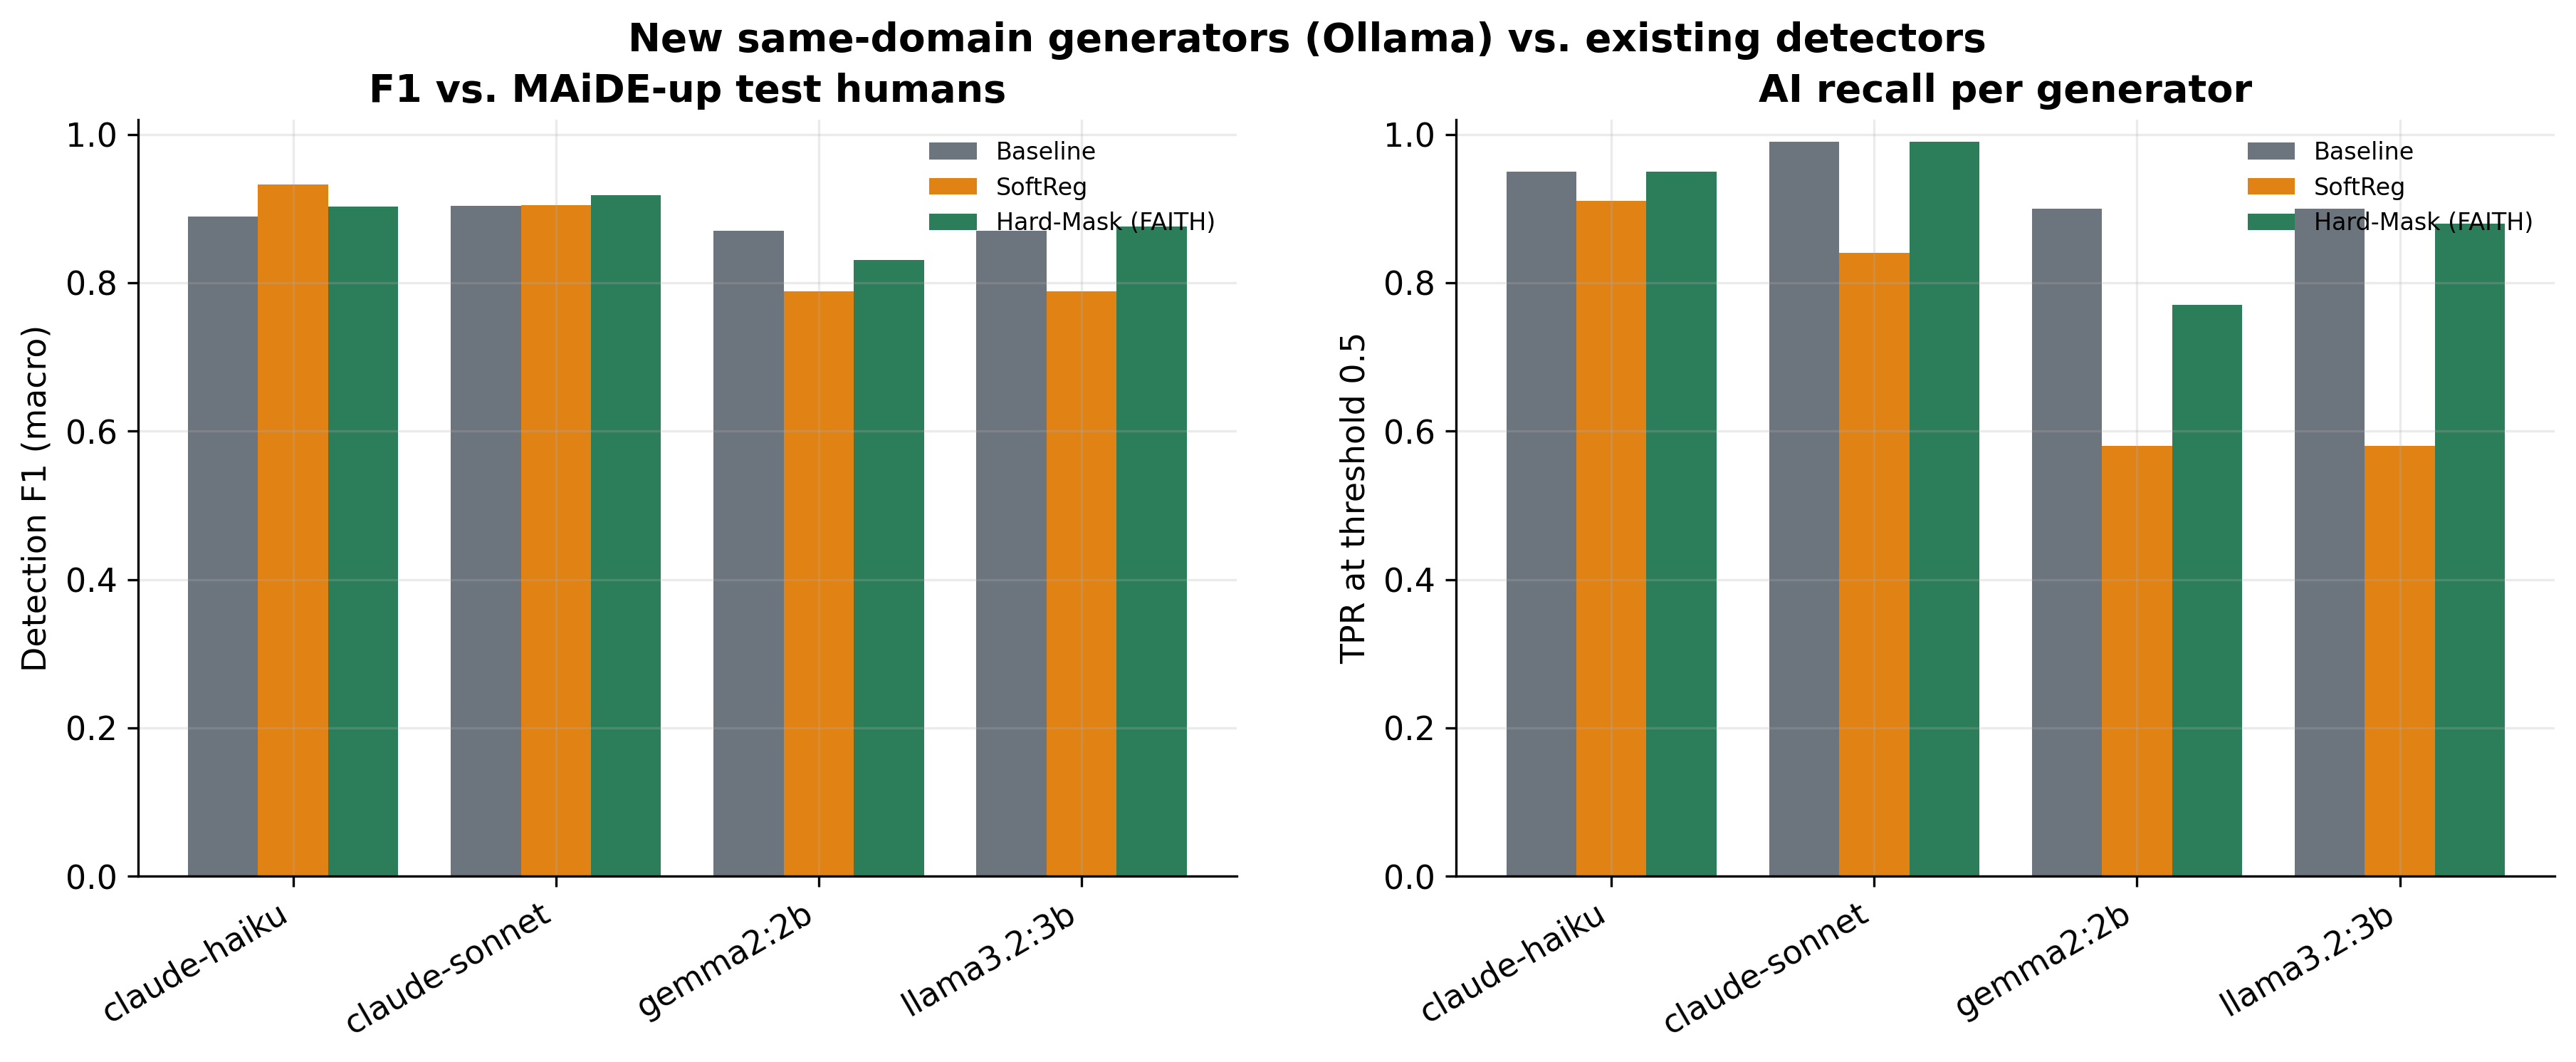
\includegraphics[width=\linewidth]{figures/18_new_generators.png}
\caption{Detection of freshly generated Llama-3.2 / Gemma-2 hotel reviews by variant.}
\label{fig:18_new_generators}
\end{figure}

\subsection{Off-the-shelf detectors}
Finally, we place our results next to existing public detectors so the reader can calibrate the absolute scores. We evaluate two pre-trained detectors zero-shot, meaning we apply them with no fine-tuning. Both were trained on other distributions, so this experiment measures how well they transfer \emph{into} our setting; it is deliberately not their best case, and we present it as a transfer test rather than a head-to-head ranking.

\begin{table*}[tp]\centering
\caption{Public pre-trained detectors applied zero-shot (\% units).}
\label{tab:offshelf}
\footnotesize
\begin{tabular}{lcccc}
\toprule
Detector & MAiDE test F1 & FW-attack & Synonym & RAID reviews \\
\midrule
chatgpt-detector-roberta & 54.9 & 35.3 & 33.9 & 70.1 \\
roberta-base-openai-detector & 40.4 & 29.3 & 46.6 & 71.2 \\
\bottomrule
\end{tabular}
\end{table*}

Two patterns stand out. First, both detectors transfer poorly into GPT-4 hotel reviews: their MAiDE F1 (54.9 and 40.4) is far below the in-domain scores our fine-tuned models reach. Second, both also degrade under the function-word attack, which extends the attack's relevance to a third, independently trained detector family and shows the vulnerability is not specific to our models. Tellingly, the same detectors recover on RAID movie reviews (70.1 and 71.2 F1), a domain much closer to their original training data. The lesson contextualises every in-domain number in this paper: detector quality is distribution-bound, performing well near its training distribution and poorly away from it. That distribution-dependence is precisely the premise of this paper's transfer analysis.

\subsection{Explanation faithfulness}\label{sec:faith}
A detector that flags a review should be able to point to the evidence behind the flag, and that evidence should be trustworthy. We therefore ask a deliberately sceptical question of every variant: when the explanation says a content word matters, does the model's prediction actually depend on it? This is the notion of \emph{faithfulness}---the degree to which an attribution reflects the computation the model truly performs, as opposed to a plausible-looking but inert highlight \cite{jacovi}. We measure it with four established, complementary metrics, all computed on content words via Integrated Gradients \cite{ig}. Comprehensiveness (higher is better) checks that removing the highlighted words hurts the prediction; sufficiency (lower is better) checks that the highlighted words alone are enough to recover it; and the deletion and insertion AUC curves \cite{rise} track how the prediction moves as words are removed from, or added back to, the input in attribution order.

\begin{table*}[tp]\centering
\caption{Explanation faithfulness (Integrated Gradients, content words). No single variant wins on all four measures: Hard-Mask leads on sufficiency and insertion, the baseline on comprehensiveness.}
\label{tab:faith}
\small
\begin{tabular}{lcccc}
\toprule
Variant & Compr.\,$\uparrow$ & Suff.\,$\downarrow$ & Del-AUC\,$\downarrow$ & Ins-AUC\,$\uparrow$ \\
\midrule
Baseline & 0.100 & 0.100 & 0.895 & 0.891 \\
SoftReg & 0.047 & 0.054 & 0.900 & 0.904 \\
Hard-Mask (FAITH) & 0.029 & -0.000 & 0.929 & 0.972 \\
\bottomrule
\end{tabular}
\end{table*}

The honest reading of Table~\ref{tab:faith} is that faithfulness is comparable across the three variants and mixed in direction (Figure~\ref{fig:09_faithfulness}). Concretely, no variant dominates on all four measures at once: Hard-Mask is strongest on sufficiency and on insertion AUC, whereas the baseline is stronger on comprehensiveness. The deletion and insertion curves (Figure~\ref{fig:10_deletion_insertion_curves}) tell the same story---the variants trace closely spaced trajectories with no clear winner. We make a point of reporting this rather than cherry-picking the metric on which our model happens to lead.

We therefore do \emph{not} claim that function-word-identity invariance buys a higher faithfulness score, and we are now in a position to be precise about what the explanation contribution is and is not. Two properties hold unconditionally. First, every attribution is computed on the deployed model itself---including its masking transform---never on a separate surrogate that might disagree with what is actually shipped (Figure~\ref{fig:14_example_explanation}); the explanation is \emph{on-model}. Second, the highlighted evidence is content-only: function-word identities can never appear in a FAITH-Detect explanation, because the hard-masked model never sees them. We deliberately call this \emph{content-displayed} rather than ``content-only faithful'': it is a property of what is shown, not a guarantee that the shown evidence captures the model's full reasoning.

That distinction matters because of the slot-reliance result (Table~\ref{tab:slotmass}). A content-only display is fully faithful only if the model's reliance on the (hidden) function-word slots is negligible---and it is \emph{not}: Hard-Mask routes $18$--$35\%$ of its attribution through the \texttt{[FUNC]} slots, which the content-only explanation does not show. So a FAITH-Detect explanation faithfully reflects the model's use of \emph{content}, but it omits a real and measurable component of the decision (how many closed-class tokens occur, and where). We thus claim only that the explanation is on-model and content-displayed, with function-word \emph{identity} provably absent from the computation; we explicitly do not claim that the displayed content words are a complete or sufficient account of the model's reasoning.

\begin{figure}[tb]\centering

\includegraphics[width=\linewidth]{figures/09_faithfulness.png}
\caption{ERASER comprehensiveness/sufficiency and deletion/insertion AUC by variant.}
\label{fig:09_faithfulness}
\end{figure}
\begin{figure*}[tp]\centering
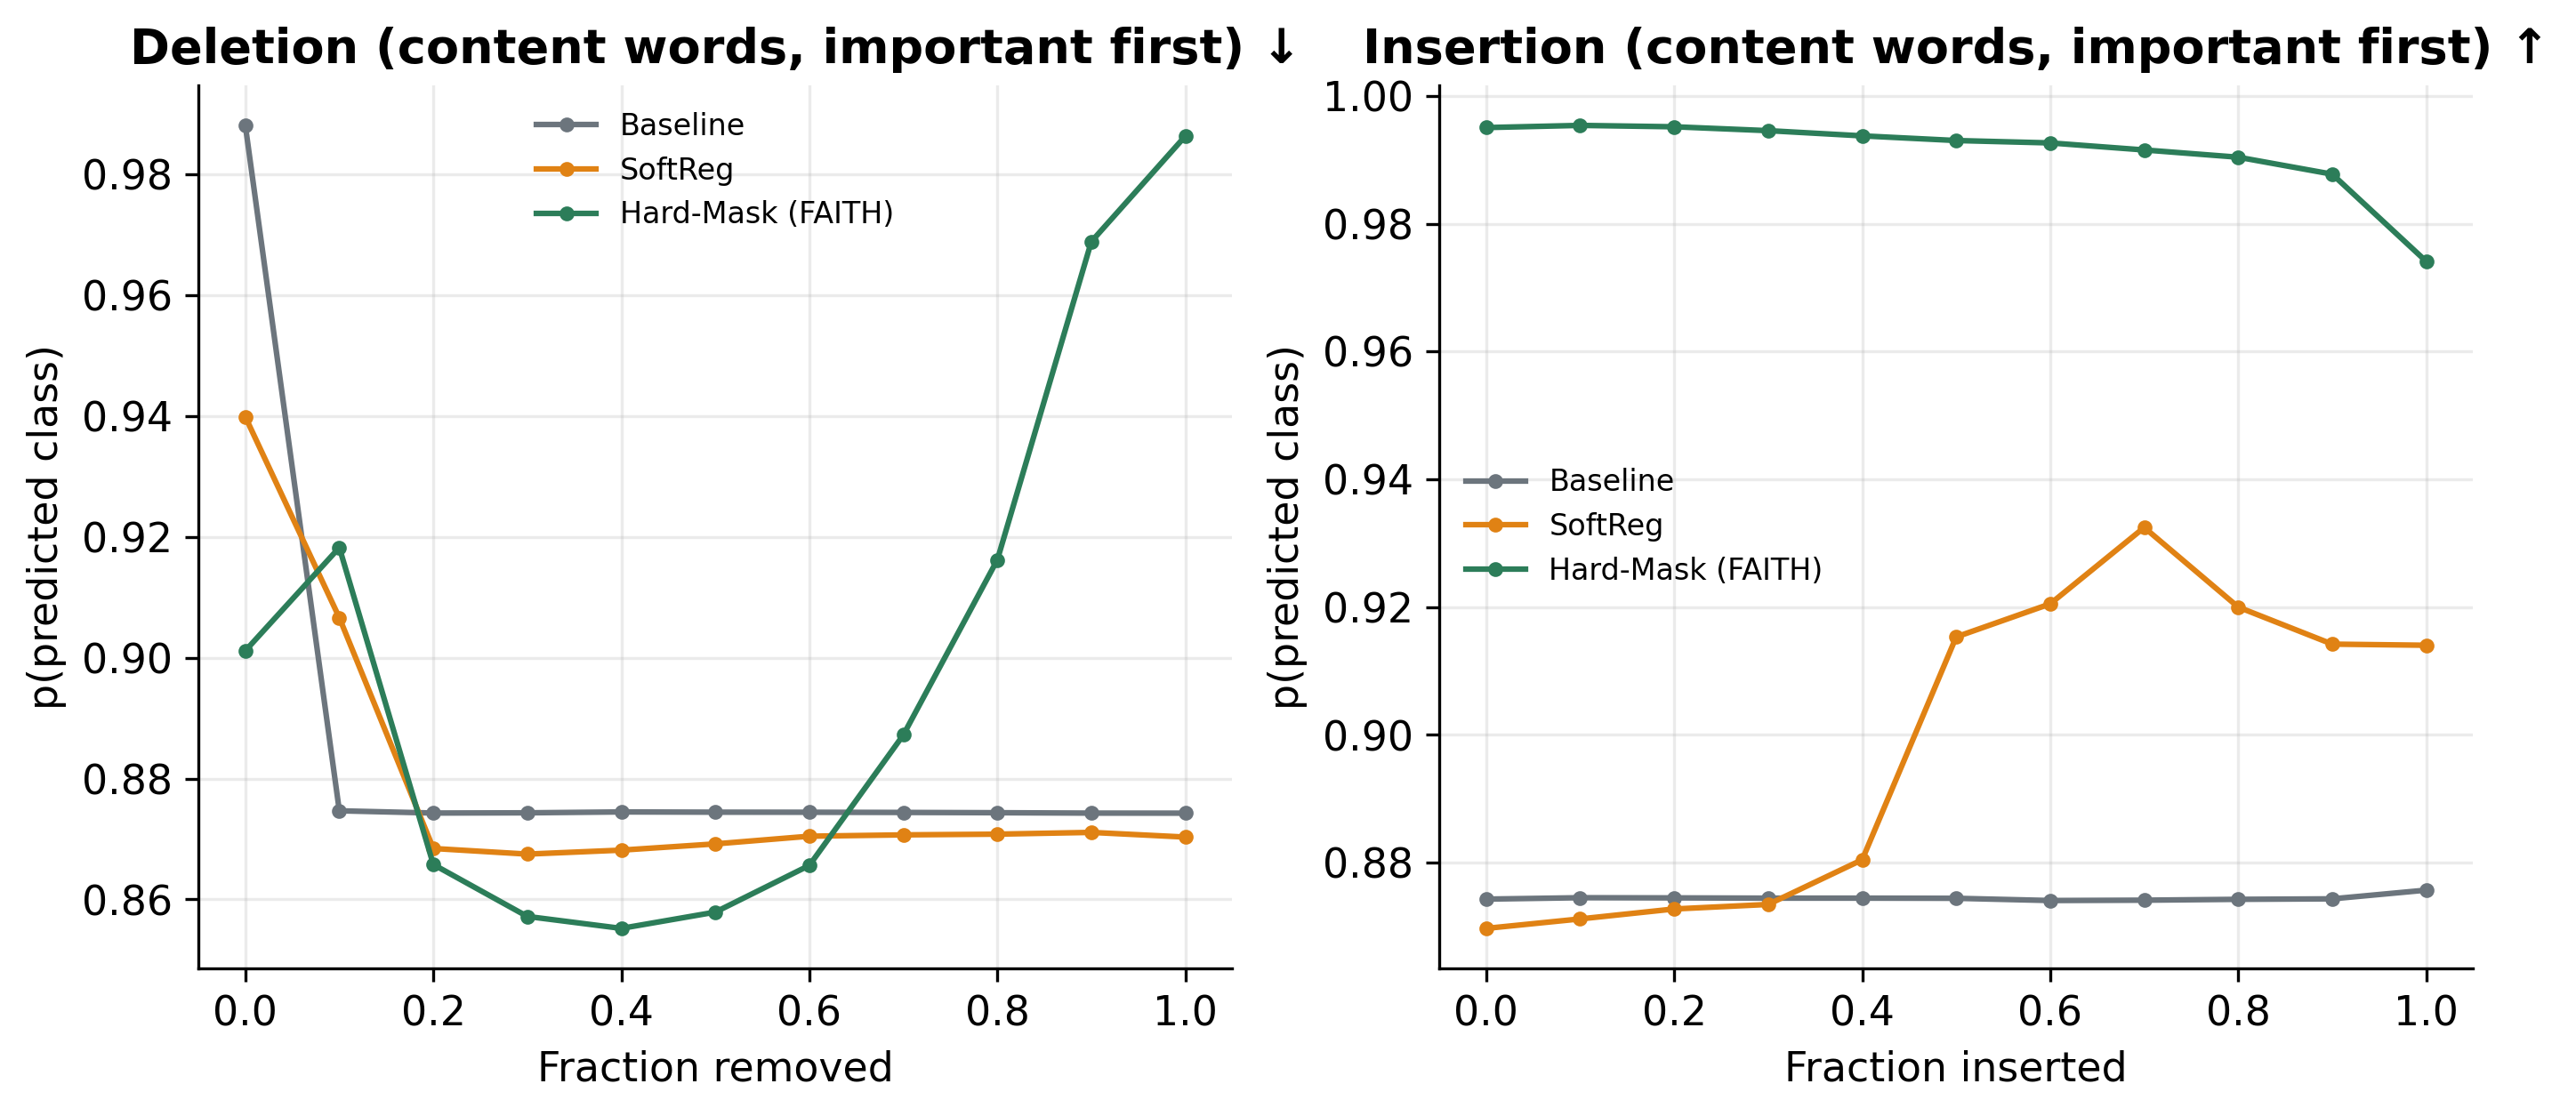
\includegraphics[width=\textwidth]{figures/10_deletion_insertion_curves.png}
\caption{Mean deletion and insertion curves over content words; the variants overlap closely, confirming comparable faithfulness.}
\label{fig:10_deletion_insertion_curves}
\end{figure*}
\begin{figure*}[tp]\centering

\includegraphics[width=\textwidth]{figures/14_example_explanation.png}
\caption{Example explanations: content words highlighted, function words greyed out and excluded by construction.}
\label{fig:14_example_explanation}
\end{figure*}
\subsection{Calibration and representation}
Beyond accuracy and faithfulness, two further properties tell us whether a detector behaves sensibly. The first is calibration: when the model reports an 80\% chance that a review is AI-generated, that confidence should be borne out roughly 80\% of the time. We summarise it with reliability diagrams and the expected calibration error \cite{guo} on the in-domain test set (Figure~\ref{fig:11_calibration}). We report calibration for completeness, so that a practitioner can judge whether the predicted probabilities are usable as confidence scores; it is not a contribution of this paper, and invariance is not designed to improve it.

The second property is how the encoder organises the reviews internally. To make this visible, we take the encoder's high-dimensional representation of each test review and project it down to two dimensions (Figure~\ref{fig:13_embedding_projection}). The picture is reassuring: for all three variants, human and AI reviews fall into well-separated clusters in-domain. This indicates that the separability we measure as F1 is reflected in the geometry of the learned representation, and---importantly---that hard masking does not collapse this structure even though it strips away function-word identity before encoding.

\begin{figure}[tb]\centering

\includegraphics[width=\linewidth]{figures/11_calibration.png}
\caption{Reliability diagrams (in-domain) with expected calibration error.}
\label{fig:11_calibration}
\end{figure}
\begin{figure*}[tp]\centering
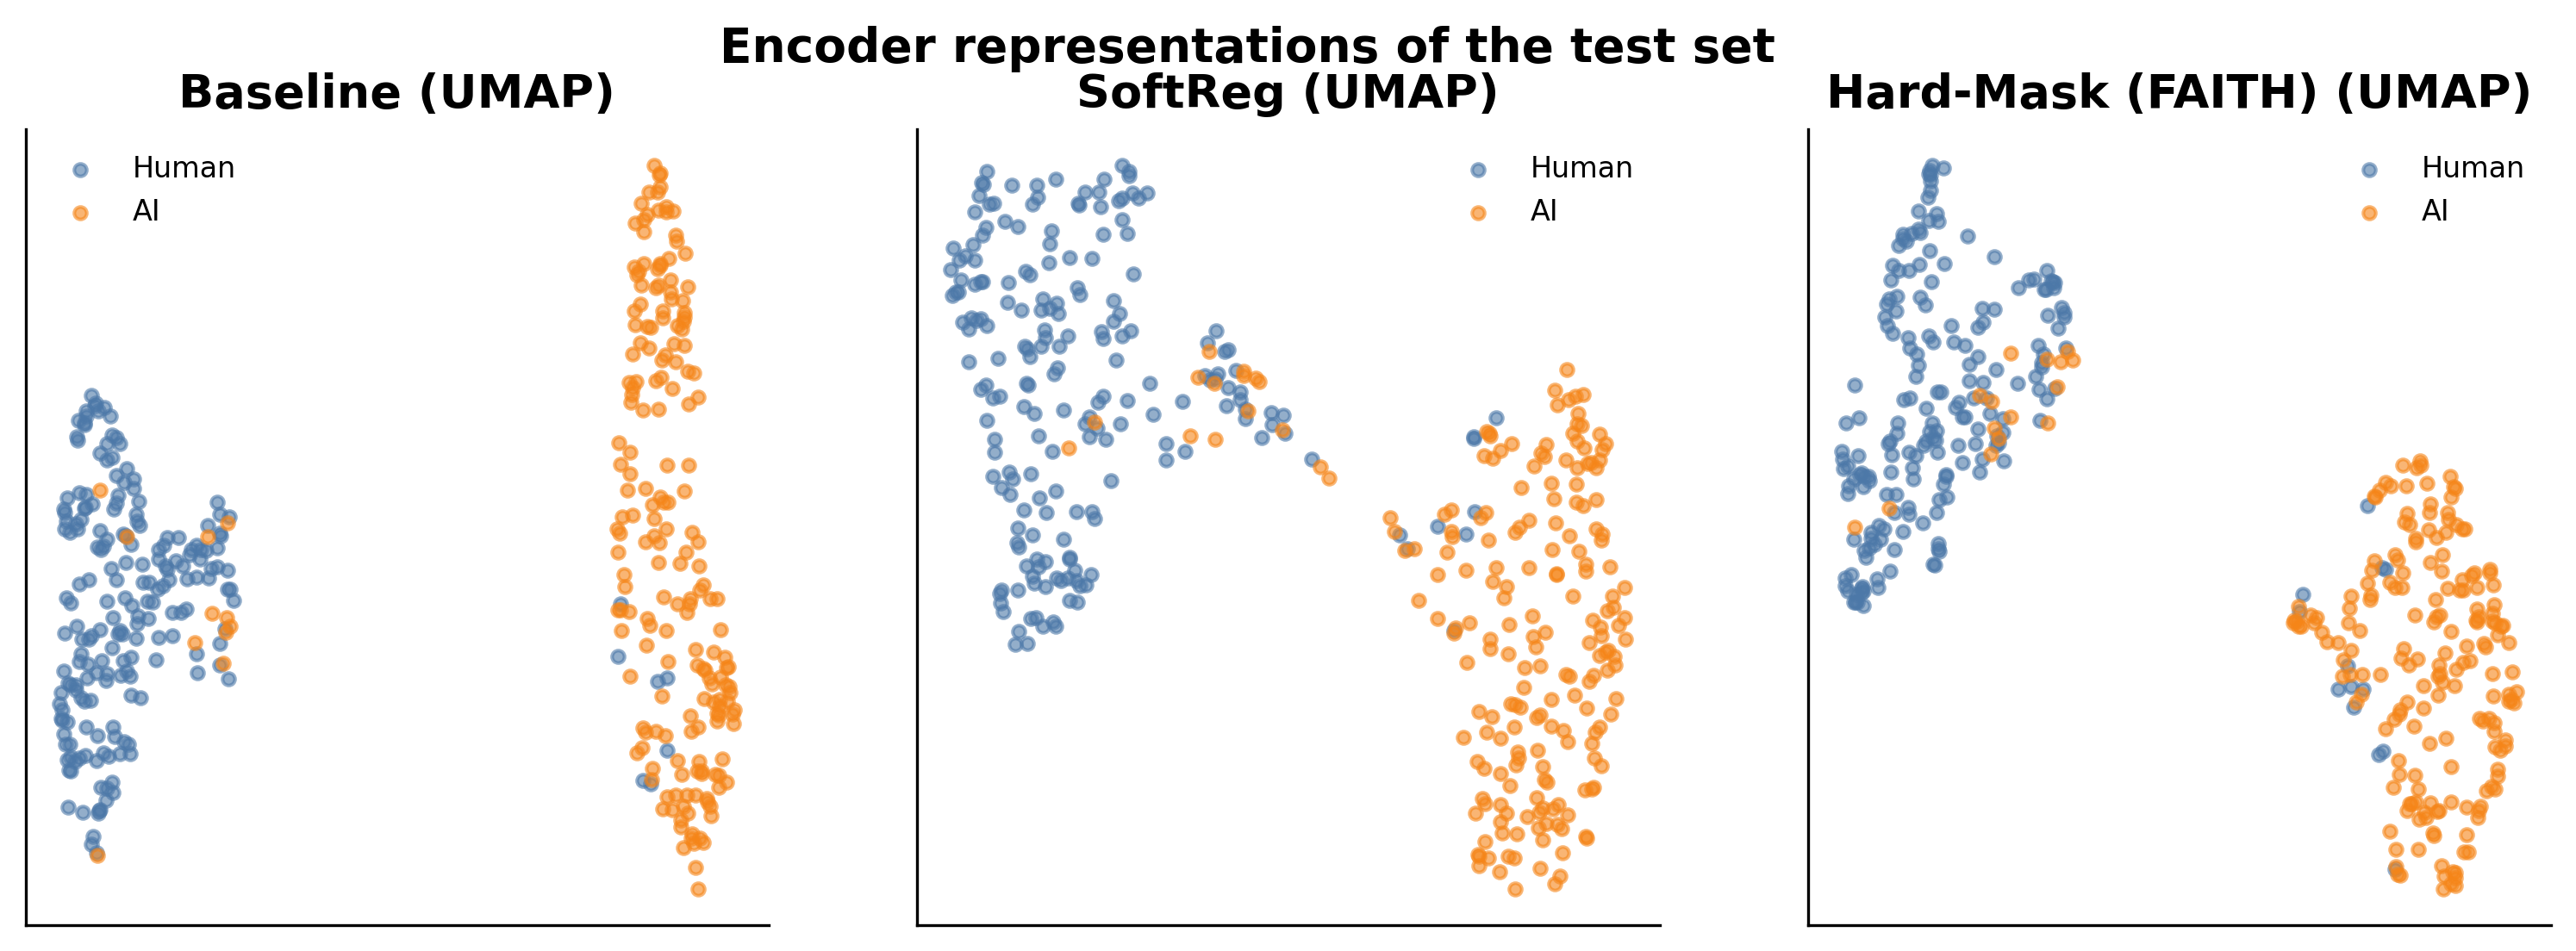
\includegraphics[width=\textwidth]{figures/13_embedding_projection.png}
\caption{Two-dimensional projection of the encoder representations of the test set; human and AI reviews separate cleanly for every variant.}
\label{fig:13_embedding_projection}
\end{figure*}
\subsection{Leakage}
A final result concerns how the dataset is split, and it is a cautionary one. The way train and test are partitioned can quietly inflate every score above. On MAiDE-up, each hotel is reviewed in both the human and the AI class, so a naive \emph{random} split scatters reviews of the same hotel across train and test. The model can then memorise hotel-specific content---names, amenities, recurring phrasing---and recognise it again at test time, which is leakage rather than genuine detection skill.

The effect is large enough to matter. A random split inflates baseline F1 to 96.7\%, against 93.2\% under the grouped, leakage-free split in which no hotel appears on both sides of the boundary (Figure~\ref{fig:02_leakage_gap}). That 3.5-point gap is purely an artefact of leakage, not improved detection. For this reason we use grouped (by-hotel) splits for every number reported in this paper, and we recommend that future work on this dataset do the same; otherwise comparisons across methods risk being dominated by how lucky each split was rather than by which detector is better.

\begin{figure}[tb]\centering
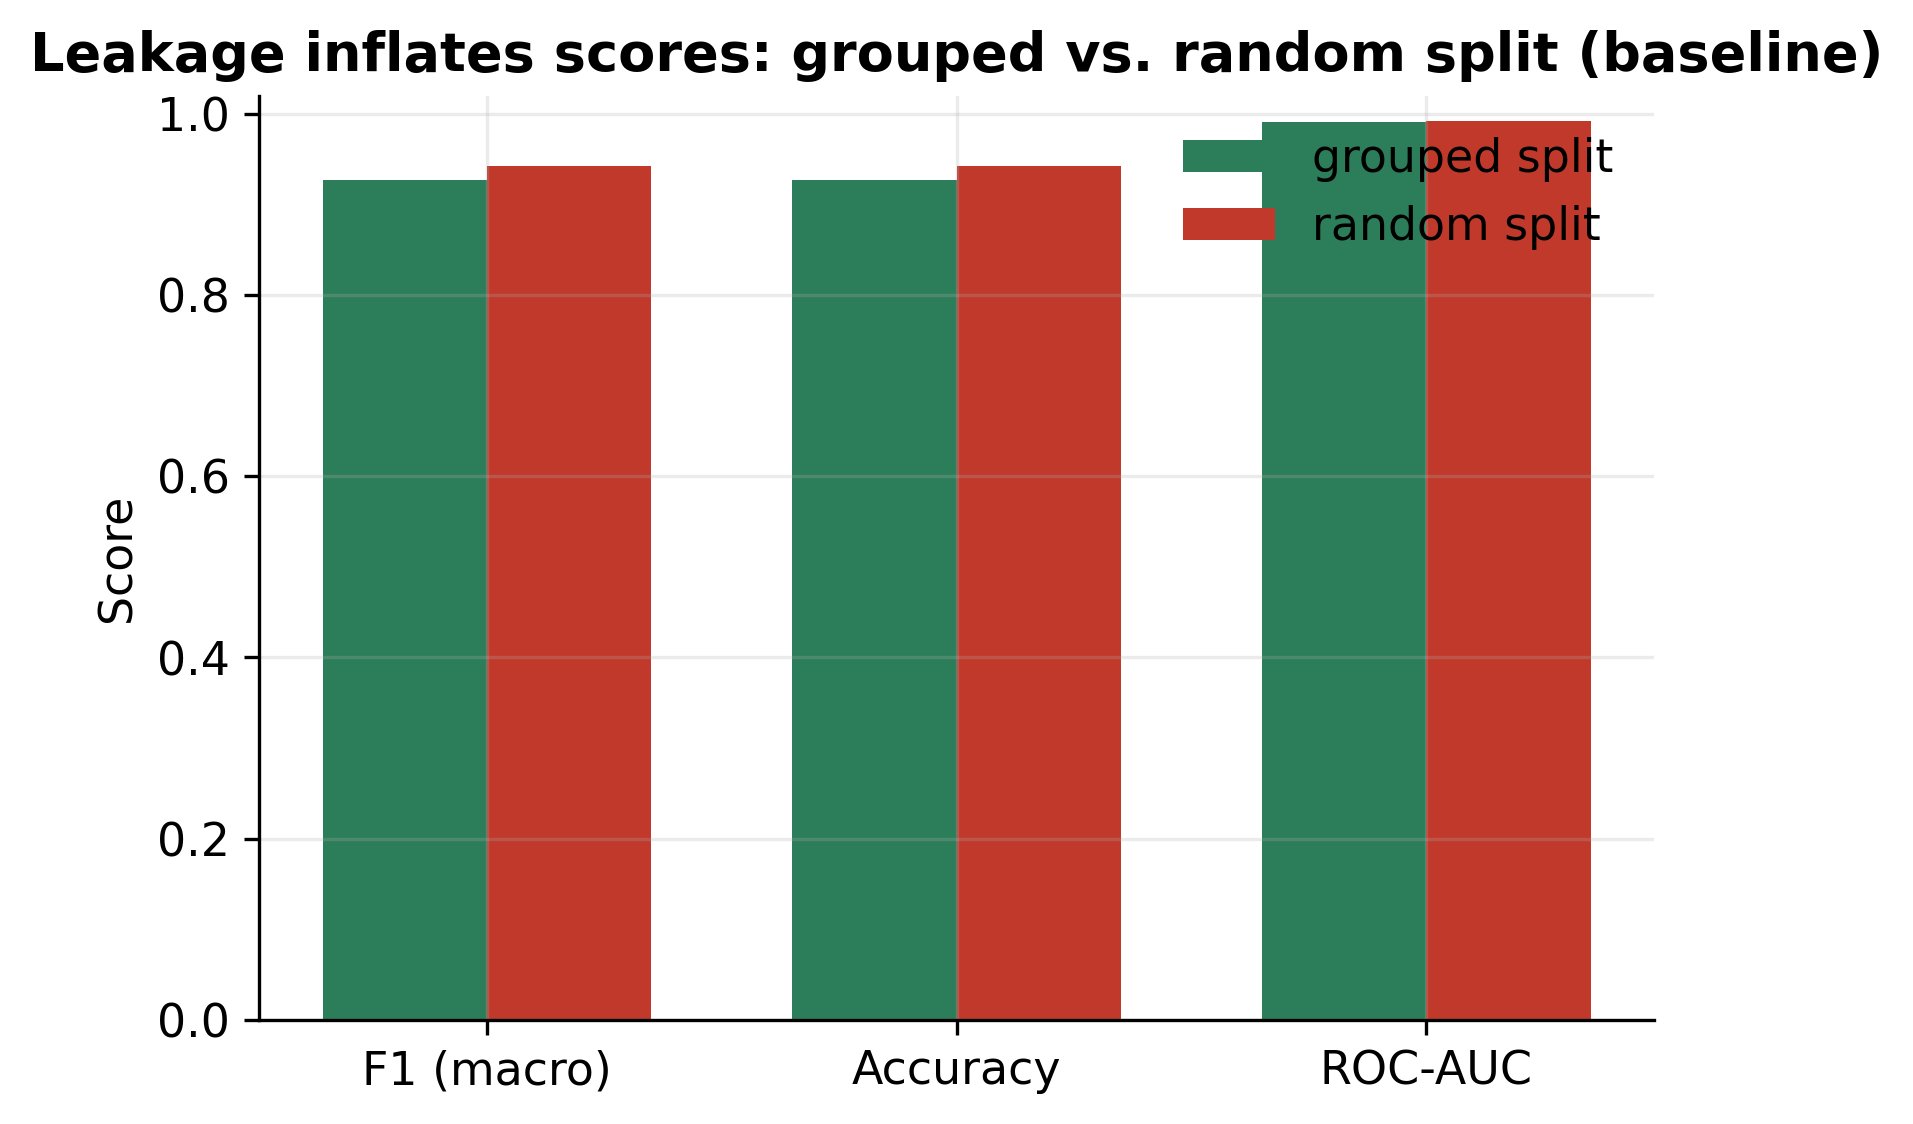
\includegraphics[width=\linewidth]{figures/02_leakage_gap.png}
\caption{Random vs.\ grouped split (baseline): random splitting overstates scores by 3.5 F1 points.}
\label{fig:02_leakage_gap}
\end{figure}

\section{Discussion}
Our results point to a single, clean conclusion: function-word-identity invariance is best understood as a trade-off, not as a free upgrade. We unpack that trade-off here and turn it into a deployment recommendation.

First, consider what invariance buys, stated precisely. In distribution, making the detector ignore function-word identity costs nothing measurable on this benchmark---the hard-masked model matches the unconstrained baseline in F1. On top of that parity, hard masking delivers a \emph{provable} guarantee: because every function word collapses to the same placeholder, the decision is invariant to function-word \emph{identity} by construction, and an automated test confirms it. That guarantee is narrow but real, and it has a matching empirical payoff: under the identity-only (swap) attack the hard-masked model is unmoved while the baseline and especially the soft variant lose ground. We are careful not to oversell the rest. The guarantee does not extend to the function-word \emph{slots}, which the model still reads (it routes $18$--$35\%$ of its attribution through them), so the model is not robust to deletion/duplication of function words, and its content-displayed explanation---computed on the deployed model, not a surrogate---is an auditability and on-model property, not a complete or fully faithful account of the decision.

Second, consider what invariance costs. The penalty appears under cross-domain shift---but it is smaller than a glance at F1 suggests. When the content vocabulary changes, the function-word and stylistic regularities that the constrained model discards do carry some domain-general signal, and the baseline exploits them. Yet the threshold-free metrics tell a milder story: Hard-Mask's OOD ROC-AUC ($0.764$) sits within noise of the baseline's ($0.780$), so the model still \emph{ranks} OOD text almost as well, and most of the F1 collapse is a miscalibrated operating point---recoverable by re-thresholding or light few-shot adaptation. Function words are thus not pure noise: in distribution they are a shortcut, but across domains some of them behave like a useful prior. This is why the constraint helps in one place and (partly, and recoverably) hurts in another.

Concretely, the choice of variant should follow the deployment setting. We recommend hard masking where robustness, auditability and a formal guarantee matter and the operating domain is fixed---for example, a single-platform review filter that must justify each flag and resist function-word tampering. Where the goal is open-domain transfer to text whose vocabulary is not known in advance, the unconstrained or soft-regularised model is the safer default, because it retains the domain-general cues that hard masking removes. The soft variant offers a middle ground: it reduces, rather than eliminates, function-word reliance and keeps the full text available.

We state these conclusions deliberately narrowly. They rest on one in-domain dataset and two attacks, and the cross-domain evidence comes from a single out-of-distribution benchmark. We therefore present invariance as a characterised design choice with a measured cost, and avoid any claim that one configuration is universally preferable.
\section{Limitations}
We close by listing the honest caveats so that the scope of our claims is unambiguous.

First, the study is English-only. Our function-word set and every experiment are built on English text, so we cannot speak to languages with different closed-class inventories or morphology.

Second, the in-domain data uses a single generator (GPT-4). As a result, our cross-generator evidence comes from a benchmark that shifts \emph{domain} at the same time as generator, and so cannot cleanly isolate generator effects; the mixed-generator pilot is a partial remedy at small scale, not a substitute for a controlled, same-domain, multi-generator in-domain corpus.

Third, the in-domain set is modest---2{,}000 reviews. Small data widens the confidence intervals we report, and we report those intervals rather than selecting favourable seeds, so the uncertainty is visible rather than hidden.

Fourth, robustness is probed with only two attacks. The function-word and synonym attacks are simple, interpretable proxies for adversarial and paraphrase pressure; they are not an exhaustive robustness audit, and a more capable attacker could behave differently.

Fifth, the faithfulness metrics are themselves contested \cite{jacovi}. We deliberately treat no single comprehensiveness, sufficiency, or deletion/insertion number as decisive, which is why our explanation contribution is framed as on-model and content-displayed rather than as a higher faithfulness score.

Sixth, invariance is to identity, not to slots. The hard-masked model still relies on the position and count of the \texttt{[FUNC]} placeholders (Table~\ref{tab:slotmass}), so the guarantee---and the robustness that follows from it---is confined to identity perturbations; a content-displayed explanation correspondingly omits this slot component of the decision.

Seventh, several analyses are pilot scale. The mixed-generator, per-category, attack-decomposition, slot-attribution, few-shot and HC3 results use distilroberta-base on a 600-review subsample (HC3: two seeds); we label them and read them as indicative, not definitive, and the HC3 transfer direction in particular is unresolved at this scale.

\paragraph{Future work.} Two of the analyses the reviewers' suggestions imply are now reported above: the masking-variant comparison that separates identity, slot-marker and position effects (\S\ref{sec:variantcmp}, Table~\ref{tab:variantcmp}) and the full-scale SoftReg $\lambda$ sweep (\S\ref{sec:lambda}, Table~\ref{tab:lambda}). One extension remains, and we release its protocol: a controlled, same-domain, multi-generator corpus evaluated at full \texttt{roberta-base} scale (held-in generators join training; a disjoint set of held-out generators forms a same-domain, different-generator test) to isolate generator shift from the domain shift that confounds the RAID OOD. We report the pilot version of this experiment in \S\ref{sec:mixedgen} and leave the full-scale run, which needs a larger same-domain generator pool than our local RAID slice provides, as the immediate next step.

Taken together, these caveats reinforce the framing of the paper: function-word-identity invariance is a design choice with a measured trade-off, not a universally preferable configuration.

\section{Conclusion}
This paper asked a deliberately narrow question: what does a detector of AI-generated reviews gain, and what does it give up, by refusing to look at function words? Our answer is concrete. First, function words are a measurable shortcut. An unconstrained detector places a large share of its attribution on closed-class tokens that human and machine writing share, and we showed at the word level that much of this signal is domain-local---it shifts, and sometimes reverses sign, when the domain changes. Second, a detector that provably ignores those tokens loses nothing in distribution: on the MAiDE-up benchmark the hard-masked model matches the unconstrained baseline in-domain, and the difference is not statistically significant.

The trade-off is what makes the result useful rather than merely cautionary. By construction, the hard-masked detector cannot read function-word \emph{identity}, so it is provably unmoved by an identity (swap) attack that costs the other variants several points, and it degrades least under synonym substitution. We are precise about the boundary: the model still uses the function-word \emph{slots} (it routes $18$--$35\%$ of its attribution through the placeholders), so the guarantee covers identity, not deletion or duplication, and its explanations are on-model and content-displayed---an auditability property---rather than a complete or higher-scoring account of the decision. The price is paid out of distribution, but is smaller than F1 implies: threshold-free ranking (ROC-AUC) barely separates the variants OOD, so most of the apparent collapse is a recoverable operating-point effect rather than lost separability. In short, function-word-identity invariance buys an explicit identity guarantee, in-domain parity, identity-attack robustness, and on-model content-displayed explanations, at a measured---and largely threshold-driven---cross-domain cost.

We therefore present function-word-identity invariance as a characterised trade-off rather than a universal improvement, and we make that characterisation the contribution. Hard masking is attractive where the domain is fixed and robustness, auditability and a constructive guarantee matter; the unconstrained or soft-regularised model remains preferable for open-domain transfer. To let others test, reuse and extend these claims, we release the code, the leakage-free grouped-split protocols, the multi-seed results with confidence intervals, and the figures, all of which regenerate from a single results file.

\paragraph{Reproducibility.} Every number in this paper is read from one results JSON; the figures and the manuscript itself regenerate from that file, so the reported values and the prose cannot drift apart. The hard-masking invariance guarantee is not asserted only in prose: an automated test checks that the model's logits are bit-identical when function words are permuted. Code, data-preparation scripts and the release protocols are available at \url{https://github.com/scar09-22/FAITH-Detect}.

\appendix
\section{Training behaviour}
This appendix records how the three variants behave during fine-tuning, complementing the final scores reported in the main text. Figure~\ref{fig:12_learning_curves} plots the training loss and the validation macro-F1 against the epoch index, averaged over the five seeds so that the curves reflect typical rather than best-case runs.

The picture is intuitive. The unconstrained baseline can use every token, including function words, from the first gradient step, so its loss falls quickly and its validation F1 climbs early. The two function-word-identity-invariant variants begin more slowly, and for a clear reason: each one removes part of the input the baseline is free to exploit. The hard-masking variant replaces every function-word sub-token with the shared \texttt{[FUNC]} placeholder, so that information is simply unavailable to the encoder; the soft variant keeps the text but penalises any saliency that lands on function words, which down-weights the same signal during training. In short, both variants must learn to separate human from machine text using content alone, and they pay for this with a slower start.

The gap is transient, not structural. As training proceeds, the constrained variants recover and converge to a validation F1 comparable to the baseline, consistent with the in-domain parity reported in Table~\ref{tab:indomain}. The early lag is therefore an optimisation effect---the constrained models take a few more epochs to find a content-only decision boundary---rather than a ceiling on what they can achieve in distribution. This is reassuring for practice: enforcing function-word-identity invariance does not require a different training budget or schedule, only patience over the first epochs.
\begin{figure}[tb]\centering

\includegraphics[width=\linewidth]{figures/12_learning_curves.png}
\caption{Training loss and validation F1 by epoch (mean over seeds). The soft and hard variants start slower because they discard or down-weight function-word information, but converge to comparable validation F1.}
\label{fig:12_learning_curves}
\end{figure}

\begin{thebibliography}{99}\small
\bibitem{maideup} O. Ignat, X. Xu, R. Mihalcea. MAiDE-up: Multilingual Deception Detection of AI-Generated Hotel Reviews. Findings of NAACL, 2025.
\bibitem{raid} L. Dugan, A. Hwang, F. Trhlik, et al. RAID: A Shared Benchmark for Robust Evaluation of Machine-Generated Text Detectors. ACL, 2024.
\bibitem{ig} M. Sundararajan, A. Taly, Q. Yan. Axiomatic Attribution for Deep Networks. ICML, 2017.
\bibitem{eraser} J. DeYoung, S. Jain, N. F. Rajani, et al. ERASER: A Benchmark to Evaluate Rationalized NLP Models. ACL, 2020.
\bibitem{ross} A. S. Ross, M. C. Hughes, F. Doshi-Velez. Right for the Right Reasons: Training Differentiable Models by Constraining their Explanations. IJCAI, 2017.
\bibitem{detectgpt} E. Mitchell, Y. Lee, A. Khazatsky, C. D. Manning, C. Finn. DetectGPT: Zero-Shot Machine-Generated Text Detection using Probability Curvature. ICML, 2023.
\bibitem{fastdetectgpt} G. Bao, Y. Zhao, Z. Teng, L. Yang, Y. Zhang. Fast-DetectGPT: Efficient Zero-Shot Detection of Machine-Generated Text via Conditional Probability Curvature. ICLR, 2024.
\bibitem{gltr} S. Gehrmann, H. Strobelt, A. M. Rush. GLTR: Statistical Detection and Visualization of Generated Text. ACL (System Demonstrations), 2019.
\bibitem{rise} V. Petsiuk, A. Das, K. Saenko. RISE: Randomized Input Sampling for Explanation of Black-box Models. BMVC, 2018.
\bibitem{geirhos} R. Geirhos, J.-H. Jacobsen, C. Michaelis, et al. Shortcut Learning in Deep Neural Networks. Nature Machine Intelligence, 2020.
\bibitem{roberta} Y. Liu, M. Ott, N. Goyal, et al. RoBERTa: A Robustly Optimized BERT Pretraining Approach. arXiv:1907.11692, 2019.
\bibitem{lime} M. T. Ribeiro, S. Singh, C. Guestrin. ``Why Should I Trust You?'': Explaining the Predictions of Any Classifier. KDD, 2016.
\bibitem{shap} S. M. Lundberg, S.-I. Lee. A Unified Approach to Interpreting Model Predictions. NeurIPS, 2017.
\bibitem{jacovi} A. Jacovi, Y. Goldberg. Towards Faithfully Interpretable NLP Systems: How Should We Define and Evaluate Faithfulness? ACL, 2020.
\bibitem{sadasivan} V. S. Sadasivan, A. Kumar, S. Balasubramanian, W. Wang, S. Feizi. Can AI-Generated Text be Reliably Detected? arXiv:2303.11156, 2023.
\bibitem{krishna} K. Krishna, Y. Song, M. Karpinska, J. Wieting, M. Iyyer. Paraphrasing Evades Detectors of AI-Generated Text, but Retrieval is an Effective Defense. NeurIPS, 2023.
\bibitem{solaiman} I. Solaiman, M. Brundage, J. Clark, et al. Release Strategies and the Social Impacts of Language Models. arXiv:1908.09203, 2019.
\bibitem{crothers} E. Crothers, N. Japkowicz, H. L. Viktor. Machine-Generated Text: A Comprehensive Survey of Threat Models and Detection Methods. IEEE Access, 2023.
\bibitem{guo} C. Guo, G. Pleiss, Y. Sun, K. Q. Weinberger. On Calibration of Modern Neural Networks. ICML, 2017.
\bibitem{gururangan} S. Gururangan, S. Swayamdipta, O. Levy, et al. Annotation Artifacts in Natural Language Inference Data. NAACL, 2018.
\bibitem{mccoy} T. McCoy, E. Pavlick, T. Linzen. Right for the Wrong Reasons: Diagnosing Syntactic Heuristics in Natural Language Inference. ACL, 2019.
\bibitem{wordnet} G. A. Miller. WordNet: A Lexical Database for English. Communications of the ACM, 1995.
\bibitem{adamw} I. Loshchilov, F. Hutter. Decoupled Weight Decay Regularization. ICLR, 2019.
\bibitem{spacy} M. Honnibal, I. Montani. spaCy: Industrial-Strength Natural Language Processing, 2017.
\end{thebibliography}

\end{document}

